% ============================================================
% main.tex — 华南理工大学本科毕业设计（论文）
% 面向高效推理的大语言模型键值缓存行为对齐量化框架
% ============================================================
\documentclass[a4paper, zihao=-4, twoside, openany, UTF8, chapter]{ctexbook}
% 注: twoside 启用偶数/奇数页页眉区分（学校规范要求）
% 若需电子版单面排版，将 twoside 改为 oneside 并删除 openany

% --- 加载配置 ---
% ============================================================
% packages.tex — 宏包集合
% ============================================================

% --- 数学 ---
\usepackage{amsmath, amssymb, amsthm}
\usepackage{bm}                  % 粗体数学符号

% --- 图表 ---
\usepackage{graphicx}
\usepackage{booktabs}            % 三线表
\usepackage{multirow}
\usepackage{makecell}            % 单元格内换行
\usepackage{tabularx}
\usepackage{longtable}
\usepackage{threeparttable}        % tablenotes 环境

% --- 浮动体 ---
\usepackage{float}
\usepackage{caption}
\usepackage{subcaption}

% --- 颜色与代码 ---
\usepackage{xcolor}
\usepackage{listings}

% --- 算法 ---
\usepackage{algorithm}
\usepackage{algpseudocode}

% --- 超链接 ---
\usepackage{hyperref}
\hypersetup{
  colorlinks=true,
  linkcolor=black,
  citecolor=black,
  urlcolor=blue,
  bookmarksnumbered=true,
}

% --- 参考文献 ---
\usepackage[sort&compress]{natbib}
\bibliographystyle{gbt7714-numerical}

% --- 绘图 ---
\usepackage{tikz}
\usetikzlibrary{arrows.meta, positioning, shapes.geometric, fit, backgrounds, calc}

% --- 其他 ---
\usepackage{enumitem}
\usepackage{url}
\usepackage{siunitx}             % 单位排版

% ============================================================
% fonts.tex — 字体设置（中文宋体，英文 Times New Roman）
% ============================================================

% --- 中文字体 ---
% 学校规范要求中文统一用宋体。标题、目录、封面标签等需要粗体处使用
% 宋体合成粗体，不再切换到黑体或楷体。
\IfFontExistsTF{Songti SC}{%
  \setCJKmainfont[AutoFakeBold=2.5, AutoFakeSlant=0.167]{Songti SC}
  \setCJKsansfont[AutoFakeBold=2.5, AutoFakeSlant=0.167]{Songti SC}
  \setCJKmonofont[AutoFakeBold=2.5, AutoFakeSlant=0.167]{Songti SC}
  \setCJKfamilyfont{zhsong}[AutoFakeBold=2.5, AutoFakeSlant=0.167]{Songti SC}
  \setCJKfamilyfont{zhhei}[AutoFakeBold=2.5, AutoFakeSlant=0.167]{Songti SC}
  \setCJKfamilyfont{zhkai}[AutoFakeBold=2.5, AutoFakeSlant=0.167]{Songti SC}
}{%
  \setCJKmainfont[AutoFakeBold=2.5, AutoFakeSlant=0.167]{FandolSong}
  \setCJKsansfont[AutoFakeBold=2.5, AutoFakeSlant=0.167]{FandolSong}
  \setCJKmonofont[AutoFakeBold=2.5, AutoFakeSlant=0.167]{FandolSong}
  \setCJKfamilyfont{zhsong}[AutoFakeBold=2.5, AutoFakeSlant=0.167]{FandolSong}
  \setCJKfamilyfont{zhhei}[AutoFakeBold=2.5, AutoFakeSlant=0.167]{FandolSong}
  \setCJKfamilyfont{zhkai}[AutoFakeBold=2.5, AutoFakeSlant=0.167]{FandolSong}
}

\providecommand{\songti}{\CJKfamily{zhsong}}
\providecommand{\heiti}{\CJKfamily{zhhei}}
\providecommand{\kaishu}{\CJKfamily{zhkai}}

% --- 英文字体 ---
% 学校规范要求: 英文字体为 Times New Roman
\setmainfont{Times New Roman}
\setsansfont{Times New Roman}
\setmonofont{Times New Roman}

% ============================================================
% format.tex — 章节标题 / 编号 / 行距 / 段落格式
% ============================================================
\usepackage{titlesec}
\usepackage{setspace}

% --- 行距：正文 1.5 倍 ---
\onehalfspacing

% --- 段落首行缩进 2 字符 ---
\setlength{\parindent}{2em}

% --- 章标题：小二号黑体，居中，单倍行距，段前段后各 0.5 行 ---
% "第X章" 格式由 ctexbook 的 chapter/name 控制
\ctexset{
  chapter = {
    format     = \centering\zihao{-2}\heiti\bfseries,
    name       = {第,章},
    number     = \chinese{chapter},
    aftername  = \quad,
    beforeskip = 0.5\baselineskip,
    afterskip  = 0.5\baselineskip,
    fixskip    = true,
  },
  section = {
    format     = \raggedright\zihao{-3}\heiti,
    beforeskip = 0.5\baselineskip,
    afterskip  = 0.5\baselineskip,
    fixskip    = true,
  },
  subsection = {
    format     = \raggedright\zihao{4}\heiti,
    beforeskip = 0.5\baselineskip,
    afterskip  = 0.5\baselineskip,
    fixskip    = true,
  },
}

% --- 图表标题格式：五号宋体，按章编号用短横线 ---
\captionsetup{
  font         = {small},          % 五号宋体（去除 sf 避免映射到黑体）
  labelsep     = quad,
  skip         = 6pt,
}
\captionsetup[figure]{
  position     = bottom,
  labelfont    = bf,
}
\captionsetup[table]{
  position     = top,
  labelfont    = bf,
}

% --- 图表按章编号 ---
\counterwithin{figure}{chapter}
\counterwithin{table}{chapter}
\counterwithin{equation}{chapter}
\renewcommand{\thefigure}{\thechapter-\arabic{figure}}
\renewcommand{\thetable}{\thechapter-\arabic{table}}
\renewcommand{\theequation}{\thechapter-\arabic{equation}}

% ============================================================
% header.tex — 页眉页脚 (fancyhdr)
% ============================================================
\usepackage{fancyhdr}

% --- 页面尺寸（A4, 上下左右各 25mm）---
\usepackage{geometry}
\geometry{
  a4paper,
  top    = 25mm,
  bottom = 25mm,
  left   = 25mm,
  right  = 25mm,
  headheight = 14pt,
  headsep    = 10mm,
  footskip   = 10mm,
}

% --- 正文页眉样式 ---
\fancypagestyle{mainmatter}{%
  \fancyhf{}%
  \fancyhead[CE]{\zihao{5}\songti 华南理工大学学士学位论文}%
  \fancyhead[CO]{\zihao{5}\songti \leftmark}%
  \fancyfoot[C]{\zihao{5}\thepage}%
  \renewcommand{\headrulewidth}{1.0pt}%
  \renewcommand{\footrulewidth}{0pt}%
}

% --- 前置部分样式（摘要/目录：罗马页码，无页眉线）---
\fancypagestyle{frontmatter}{%
  \fancyhf{}%
  \fancyfoot[C]{\zihao{5}\thepage}%
  \renewcommand{\headrulewidth}{0pt}%
  \renewcommand{\footrulewidth}{0pt}%
}

% --- 空白页样式 ---
\fancypagestyle{plain}{%
  \fancyhf{}%
  \fancyfoot[C]{\zihao{5}\thepage}%
  \renewcommand{\headrulewidth}{0pt}%
  \renewcommand{\footrulewidth}{0pt}%
}

% ============================================================
% toc.tex — 目录格式 (tocloft)
% ============================================================
\usepackage{tocloft}

% --- 目录标题：小二号黑体居中 ---
\renewcommand{\cfttoctitlefont}{\hfill\zihao{-2}\heiti\bfseries}
\renewcommand{\cftaftertoctitle}{\hfill}

% --- 章条目：四号黑体 ---
\renewcommand{\cftchapfont}{\zihao{4}\heiti}
\renewcommand{\cftchappagefont}{\zihao{4}\normalfont}
\renewcommand{\cftchapleader}{\cftdotfill{\cftdotsep}}

% --- 节条目：小四号宋体 ---
\renewcommand{\cftsecfont}{\zihao{-4}\songti}
\renewcommand{\cftsecpagefont}{\zihao{-4}\normalfont}

% --- 条条目：小四号宋体 ---
\renewcommand{\cftsubsecfont}{\zihao{-4}\songti}
\renewcommand{\cftsubsecpagefont}{\zihao{-4}\normalfont}

% --- 行距 1.5 倍 ---
\setlength{\cftbeforechapskip}{0pt}
\setlength{\cftbeforesecskip}{0pt}
\setlength{\cftbeforesubsecskip}{0pt}

% --- 目录深度到 subsection ---
\setcounter{tocdepth}{2}

% ============================================================
% commands.tex — 自定义命令与环境
% ============================================================

% === 封面信息变量 ===
\newcommand{\thesistitle}{面向高效推理的大语言模型键值缓存行为对齐量化框架}
\newcommand{\thesisauthor}{陈梓浪}
\newcommand{\thesisstudentid}{202264642457}
\newcommand{\thesiscollege}{吴贤铭智能工程学院}
\newcommand{\thesismajor}{智能制造工程}
\newcommand{\thesissupervisor}{曾子倩}
\newcommand{\thesissubmitdate}{2026年6月}

% === 封面 ===
\newcommand{\makecover}{%
  \begin{titlepage}
    \centering
    \vspace*{2cm}
    {\zihao{1}\heiti\bfseries 华南理工大学} \\[0.5cm]
    {\zihao{2}\heiti 本科毕业设计（论文）} \\[3cm]
    {\zihao{2}\heiti\bfseries \thesistitle} \\[4cm]
    \begin{tabular}{rl}
      {\zihao{4}\heiti 学\qquad 院：} & {\zihao{4}\songti \thesiscollege} \\[0.5em]
      {\zihao{4}\heiti 专\qquad 业：} & {\zihao{4}\songti \thesismajor} \\[0.5em]
      {\zihao{4}\heiti 学生姓名：}    & {\zihao{4}\songti \thesisauthor} \\[0.5em]
      {\zihao{4}\heiti 学生学号：}    & {\zihao{4}\songti \thesisstudentid} \\[0.5em]
      {\zihao{4}\heiti 指导教师：}    & {\zihao{4}\songti \thesissupervisor} \\[0.5em]
      {\zihao{4}\heiti 提交日期：}    & {\zihao{4}\songti \thesissubmitdate} \\
    \end{tabular}
  \end{titlepage}
}

% === 原创性声明 ===
\newcommand{\makedeclaration}{%
  \clearpage
  \thispagestyle{empty}
  \begin{center}
    {\zihao{2}\heiti 华南理工大学\\学位论文原创性声明}
  \end{center}
  \vspace{0.5\baselineskip}
  \zihao{4}\songti\setlength{\parindent}{2em}

  本人郑重声明：所呈交的论文是本人在导师的指导下独立进行研究所取得的研究成果。
  除了文中特别加以标注引用的内容外，本论文不包含任何其他个人或集体已经发表或撰写的成果作品。
  对本文的研究做出重要贡献的个人和集体，均已在文中以明确方式标明。
  本人完全意识到本声明的法律后果由本人承担。

  \vspace{2cm}
  \begin{flushright}
    作者签名：\underline{\hspace{4cm}} \qquad 日期：\underline{\hspace{2cm}}年\underline{\hspace{1cm}}月\underline{\hspace{1cm}}日
  \end{flushright}

  \vspace{2cm}
  \begin{center}
    {\zihao{2}\heiti 学位论文版权使用授权书}
  \end{center}
  \vspace{0.5\baselineskip}

  本学位论文作者完全了解学校有关保留、使用学位论文的规定，即：学校有权保存并向国家有关部门或机构送交论文的复印件和电子版，
  允许学位论文被查阅；学校可以公布学位论文的全部或部分内容，可以允许采用影印、缩印或其它复制手段保存、汇编学位论文。
  本人电子文档的内容和纸质论文的内容相一致。

  \vspace{2cm}
  \begin{flushright}
    作者签名：\underline{\hspace{4cm}} \qquad 日期：\underline{\hspace{2cm}}年\underline{\hspace{1cm}}月\underline{\hspace{1cm}}日 \\[1em]
    指导教师签名：\underline{\hspace{4cm}} \qquad 日期：\underline{\hspace{2cm}}年\underline{\hspace{1cm}}月\underline{\hspace{1cm}}日
  \end{flushright}
}

% === 中文摘要环境 ===
\newenvironment{abstractzh}{%
  \clearpage
  \begin{center}
    {\zihao{-2}\heiti\bfseries 摘\qquad 要}
  \end{center}
  \vspace{0.5\baselineskip}
  \zihao{-4}\songti\setlength{\parindent}{2em}
}{}

% === 中文关键词 ===
\newcommand{\keywordszh}[1]{%
  \par\vspace{0.5\baselineskip}\noindent
  {\zihao{-4}\heiti 关键词：}{\zihao{-4}\songti #1}
}

% === 英文摘要环境 ===
\newenvironment{abstracten}{%
  \clearpage
  \begin{center}
    {\zihao{-2}\bfseries Abstract}
  \end{center}
  \vspace{0.5\baselineskip}
  \zihao{-4}\setlength{\parindent}{2em}
}{}

% === 英文关键词 ===
\newcommand{\keywordsen}[1]{%
  \par\vspace{0.5\baselineskip}\noindent
  {\zihao{-4}\bfseries Keywords: }{\zihao{-4} #1}
}

% === 致谢环境 ===
\newenvironment{acknowledgements}{%
  \clearpage
  \chapter*{致\qquad 谢}
  \addcontentsline{toc}{chapter}{致谢}
  \zihao{-4}\songti\setlength{\parindent}{2em}
}{}

% === 常用缩写 ===
\newcommand{\ie}{\textit{i.e.}}
\newcommand{\eg}{\textit{e.g.}}
\newcommand{\etal}{\textit{et al.}}
\newcommand{\cf}{\textit{cf.}}

% === 数学符号 ===
\newcommand{\bx}{\bm{x}}
\newcommand{\bq}{\bm{q}}
\newcommand{\bk}{\bm{k}}
\newcommand{\bv}{\bm{v}}
\newcommand{\bK}{\bm{K}}
\newcommand{\bV}{\bm{V}}
\newcommand{\bQ}{\bm{Q}}
\newcommand{\bO}{\bm{O}}
\DeclareMathOperator{\softmax}{softmax}
\DeclareMathOperator{\KL}{KL}
\DeclareMathOperator*{\argmin}{arg\,min}

% === 代码/函数名排版（正体 Times New Roman，融入正文） ===
\newcommand{\code}[1]{\textrm{#1}}


% ============================================================
\begin{document}

% === 封面（不编页码）===
\makecover

% === 原创性声明（不编页码）===
\makedeclaration

% === 前置部分（罗马页码）===
\frontmatter
\pagestyle{frontmatter}

% --- 中文摘要 ---
% Chinese abstract.

\begin{abstractzh}

随着大语言模型长上下文推理窗口不断扩大，自回归推理过程中键值缓存的显存占用不断增加。在真实模型部署场景中，算力硬件的显存逐渐难以满足推理需要。虽然降低缓存位宽能够直接减少显存占用，但因为 Key 侧扰动可能经 logits 与 softmax 改写注意力分布，Value 侧扰动通过加权聚合影响输出表示，现有量化路径常用的张量级重建误差校准并不一定能充分展示量化缓存进入注意力计算后的功能偏移。本文提出一种面向高效推理的 KV Cache 行为对齐量化框架，将注意力分布、聚合输出与任务表现作为共同的校准标准，连接量化参数选择、低比特恢复和量化预算分配三个决策环节。

本文使用校准样本评估全精度参考配置与候选量化配置，记录 attention-distribution KL 与注意力聚合输出扰动两类读数用于筛选量化校准参数，保留下游任务读数作为任务层面的审计依据。然后把校准阶段得到的逐层读数进一步汇总为层级行为敏感度，形成跨模型维度敏感度画像图谱，从而观察不同模型的关键层分布形态。并利用画像图谱在固定 $k$ 预算下比较行为引导分配与位置启发式基线，提出通过 \texttt{AutoK} 根据敏感度排序和覆盖率阈值自动生成模型级 $k$ 候选。构建了一套离线行为读数，同时实现保真校准、低比特行为恢复、跨模型结构判读和预算候选生成，使量化路径与层间预算建议形成连续证据链。

本文的实验覆盖 Qwen2.5、LLaMA-3.1 与 Mistral 三个模型族的六个开源指令模型，结果显示 KV Cache 量化和预算分配都具有明显的模型族、规模和任务依赖性。行为引导校准在保守量化位宽INT8下能够保持稳定保真，进入 \texttt{INT4} 后，对称量化在 Qwen 系列中出现检索阶跃崩塌，K/V 角色诊断表明 Key 侧低比特噪声是直接的失稳触发源，采用角色感知低比特路径 \texttt{INT4-RoleAlign} 可将检索行为恢复到可用区间。跨模型预算实验中自动参数选择 \texttt{AutoK} 效果最好的是模型Mistral-7B，Qwen2.5-3B 对应早层保护有效区间，LLaMA-3.1-8B 呈现中等规模共识区间，Qwen2.5-14B 则表现为高性能簇接近而无稳定最优。\texttt{INT4} 路径可带来约 $73.4\%$ 的 KV Cache 容量压缩，但融合解码的时间收益受 $H_{kv}$、序列长度和后端实现共同影响。
总体而言，本文验证了一条以注意力行为保持为核心、以 K/V 角色差异恢复为低比特路径、以 \texttt{AutoK} 和行为敏感度画像为预算接口的 KV Cache 行为对齐量化框架。

\keywordszh{大语言模型；KV Cache 量化；注意力行为保持；低比特推理；行为引导校准；预算分配}

\end{abstractzh}


% --- 英文摘要 ---
% English abstract.

\begin{abstracten}

As long-context inference expands, the KV cache in autoregressive decoding grows with sequence length, shifting the deployment bottleneck from computation toward cache storage and memory access. Reducing cache bit-width lowers memory footprint, but tensor-level reconstruction error does not fully capture functional shifts after the quantized cache enters attention. Key perturbations can reshape logits and softmax attention distributions, while Value perturbations mainly affect output representations through weighted aggregation. This thesis proposes a behavior-aligned KV-cache quantization framework for efficient inference, using attention distributions, aggregation outputs, and task behavior as shared calibration and auditing targets across quantization-parameter selection, low-bit recovery, and layer-wise budget allocation.

Using calibration samples, this thesis evaluates full-precision reference and candidate quantized configurations in parallel. It records attention KL divergence and aggregation-output perturbation as fidelity readings for calibration-parameter selection, while retaining downstream task scores as audit signals. Layer-wise readings are then summarized into behavioral sensitivity profiles and assembled across models into a sensitivity-profile map, which exposes critical-layer distributions under different model conditions. This map supports fixed-$k$ comparisons between behavior-guided allocation and positional heuristics, and lets \texttt{AutoK} generate model-level $k$ candidates from sensitivity rankings and coverage thresholds. Thus, one set of offline behavioral readings supports fidelity calibration, low-bit behavior recovery, cross-model structural interpretation, and budget candidate generation.

Experiments cover six open-source instruction models from the Qwen2.5, LLaMA-3.1, and Mistral families, and show clear family-, scale-, and task-dependent behavior in KV-cache quantization and budget allocation. On the Qwen2.5-1.5B task-core protocol, the INT8 baseline differs from \texttt{FP16} by about $+0.02$ in the three-task mean, showing stable fidelity under conservative bit-width. With \texttt{INT4}, symmetric quantization causes stepwise retrieval collapse on Qwen models; K/V diagnostics identify Key-side low-bit noise as the direct trigger, and \texttt{INT4-RoleAlign} restores usable retrieval. Cross-model allocation maps four regimes: \texttt{AutoK} is clearest on Mistral-7B, Qwen2.5-3B favors early-layer protection, LLaMA-3.1-8B forms a medium-scale consensus regime, and Qwen2.5-14B shows nearby high-performance clusters without a stable winner. The \texttt{INT4} path yields about $73.4\%$ KV-cache capacity compression, while fused-decode time gains depend on $H_{kv}$, sequence length, and backend implementation. Overall, this thesis validates a behavior-aligned KV-cache quantization framework centered on attention-behavior preservation, K/V role-aware low-bit recovery, and \texttt{AutoK} with behavioral sensitivity profiles as the budget interface.

\keywordsen{large language models, KV-cache quantization,
attention-behavior preservation, low-bit inference,
behavior-guided calibration, budget allocation}

\end{abstracten}


\clearpage   % 英文摘要与目录分页

% --- 目录 ---
\tableofcontents

% === 正文（阿拉伯页码 + 页眉）===
\mainmatter
\pagestyle{mainmatter}

% ============================================================
% ch1_introduction.tex — 第一章 绪论
% ============================================================
\chapter{绪论}

\section{研究背景}

长上下文推理把大语言模型（Large Language Model, LLM）的部署压力集中到解码阶段。LLaMA~3~\cite{grattafiori2024llama3}、Qwen2.5~\cite{qwen2025qwen25} 等模型已经能够处理更长输入，但在自回归生成中，每个新 token 都要访问此前累积的缓存。对本文而言，部署压力的直接落点是：当上下文长度和服务并发同步上升时，Decode 阶段需要反复读取的 KV Cache 字节数会怎样限制可部署性。

Transformer~\cite{vaswani2017attention} 自回归解码的计算路径决定了这一压力的来源。第 $t$ 个生成步只新增当前位置的 Query、Key 和 Value，但注意力仍需访问前 $S$ 个历史位置的 Key/Value。KV Cache 避免了重复执行历史 K/V 投影，却把缓存容量与访存带宽变成每个 decode step 都要面对的约束。也就是说，缓存不是只在 prefill 后静态占用显存；它还会在后续 token 生成中持续参与注意力计算。

从存储结构上看，KV Cache 的显存占用与模型层数、每层 KV 头数、头维度、序列长度以及存储精度近似成正比，可写为
\begin{equation}
  M_{\mathrm{KV}} = 2 \times L \times H_{kv} \times d_k \times S \times b
  \label{eq:kv_memory}
\end{equation}
其中 $L$、$H_{kv}$ 与 $d_k$ 由模型结构给定，$S$ 对应上下文长度，$b$ 对应缓存元素的存储字节数，系数 2 来自 Key 与 Value 两部分。本文使用式~\eqref{eq:kv_memory} 固定后续实验变量：模型结构决定基础缓存形状，序列长度与 batch size 决定部署压力，量化位宽直接改变 $b$，而预算分配方法则决定哪些层或角色保留更高精度。在长上下文和批量推理场景下，这一开销会随上下文长度与并发批次同步放大。vLLM~\cite{kwon2023vllm} 等推理框架通过分页注意力（PagedAttention）改善显存碎片和缓存管理效率，但这类方法并不直接减少 KV Cache 的绝对存储量。

因此，KV Cache 量化的系统价值首先来自它直接作用于 $b$。INT8 可以提供相对保守的缓存压缩锚点，INT4 则进一步压低存储字节数，也更容易暴露低比特扰动在注意力计算中的后果。本文后续不把“位宽更低”等同于“路径更好”，而是把 Decode 阶段缓存字节数、注意力行为稳定性和任务读数放在同一套实验口径下比较。

\section{问题定义与研究动机}

在上述背景下，KV Cache 量化的价值首先来自直接的存储压缩。INT8 可以作为较保守的保真基线，更低位宽则能进一步释放显存空间，支持更长上下文或更高并发。但缓存压缩不能只按 bit 数下降来理解：位宽降低以后，Key 与 Value 的扰动会进入注意力计算，并可能改变检索、摘要和语言建模等任务行为。本文后续以 INT4 作为低比特压力点，正是因为这一设置会更清楚地暴露 Key/Value 角色差异和模型间敏感度差异；后文的 Qwen 与 LLaMA 对照会把这种差异落到 \texttt{K4V8}/\texttt{K4V4} 等布局上，此处只把它作为问题线索，并保留架构调制的解释空间。

当前 KV Cache 量化的校准目标仍常落在数值重建误差上，典型做法包括 MSE 损失和基于分位数的裁剪。这类做法通常把“张量越接近原值，模型行为越接近全精度路径”作为工作前提。进入注意力计算后，这个前提并不总稳固：softmax 的非线性可能把较小的 Key 扰动转化为注意力概率的明显变化，而某些数值上更大的误差又可能在归一化中被部分吸收。因此，张量误差大小与下游功能偏移之间难以建立稳定的一一对应关系；不同层、不同头和不同上下文位置上的分布差异，也会进一步削弱静态阈值的解释力。

KV Cache 量化的困难因此不只是继续调节超参数或压低重建误差。模型在推理时感知到的是量化误差经过注意力计算后的功能偏移：注意力分布是否被重排，聚合输出是否偏离，任务行为是否随之改变。特别是在长上下文和低比特场景下，同一量级的数值扰动落在不同层、不同头或不同角色上，可能产生完全不同的后果。单纯追求全局数值误差最小，并不能保证模型在推理时保持稳定和可用。

这使本文把观察对象从单纯的张量近似扩展到推理行为本身：KV Cache 量化在保持重建精度之外，还需要尽量维持注意力分布、聚合输出和任务表现的稳定。量化后注意力分布是否发生重排、这种重排是否继续影响输出与任务结果，是更贴近推理可用性的观察依据。后续关于校准目标、量化路径和预算分配的讨论，也以这些行为读数作为共同依据。

为避免“行为”停留在抽象表述，本文将注意力行为操作化为三类可观测量：其一是量化前后注意力分布的偏移，用于刻画检索和排序关系是否被扰动；其二是加权聚合输出的变化，用于刻画 Value 信息进入残差流后的表示偏移；其三是语言建模、检索和长文档任务上的表现变化，用于检验上述扰动是否传导到任务层面。进一步地，本文所说的行为敏感度画像，是指由离线校准与诊断读数聚合得到的逐层相对敏感度，用于回答哪些层或角色应被优先保护；策略适用区间则指在特定模型家族、规模、任务和预算条件下，不同预算策略进入高性能区域的条件范围。

基于这一问题意识，下一节只做必要的相关研究定位：已有工作分别回答低比特表示、缓存压缩格式和系统执行效率问题，而本文要接上的缝隙是量化缓存进入注意力计算后如何保持推理行为。

\section{国内外研究现状概述}

围绕长上下文推理与 KV Cache 压缩，现有研究主要回答三个相邻但不同的问题。模型量化研究提供低比特表示、校准与误差控制的基础方法；KV Cache 专属量化直接处理缓存存储压力；高效推理系统则从注意力计算和缓存管理角度降低部署开销。三条路线的交集说明，长上下文部署由压缩精度、缓存组织和系统执行共同决定。

在模型量化方向，已有研究围绕权重与激活的低比特表示、训练后量化以及校准策略形成了较为成熟的方法体系。以 SmoothQuant~\cite{xiao2023smoothquant}、GPTQ~\cite{frantar2023gptq} 和 AWQ~\cite{lin2024awq} 为代表的工作，分别从量化难度转移、近似误差补偿和激活感知保护等角度推进了大模型的压缩与部署。这些方法主要面向模型参数与激活，但其中关于量化表示、误差控制和校准流程的基本思想，也为后续 KV Cache 压缩提供了重要的方法学参考。

在 KV Cache 专属量化方向，随着长上下文推理对缓存显存的压力持续上升，研究开始直接面向缓存本身设计压缩路径。KIVI~\cite{liu2024kivi} 强调 K/V 统计差异与异构量化轴，KVQuant~\cite{hooper2024kvquant} 关注极低比特表示中的码本和误差补偿，ZipCache~\cite{he2024zipcache} 则从重要性驱动的缓存压缩切入。这些工作留下的共同问题是：当缓存扰动通过 softmax 和加权聚合进入推理行为时，校准与格式选择应如何被审计。

除量化压缩外，高效推理方向也在同步推进。FlashAttention~\cite{dao2022flashattention,dao2024flashattention2} 通过更高效的分块注意力计算降低中间访存开销；分页注意力~\cite{kwon2023vllm} 则通过缓存分页改善显存碎片和缓存利用率。这类工作与 KV Cache 量化并非替代关系，而是从不同层面共同服务于长上下文推理的可部署性。

现有研究已经从模型量化、KV Cache 专属压缩与高效推理等角度推进了长上下文部署，但这些路线解决的层面并不相同。本文的切入点是 KV Cache 量化中的行为保持问题：量化后的缓存不仅要占用更少显存，还要在注意力计算中保持可用的推理行为。下面的研究问题从这一观察出发，而不是预设某一种量化格式或预算策略会在所有模型上占优。

\section{核心假设与研究问题}

KV Cache 量化的核心难点不只是继续提高压缩率，而是如何在压缩后保持模型的实际推理行为。本文把注意力行为作为分析起点，关注量化后注意力分布、聚合输出和任务表现是否仍与全精度路径保持一致。

\noindent\textbf{核心假设：} 在 KV Cache 量化中，注意力行为比张量重建误差更接近模型实际功能损伤。本文关心量化后注意力分布是否保持稳定、加权聚合输出是否偏离，以及这些变化是否影响任务行为。基于这一假设，校准目标和预算分配可以共享同一个观察对象，而不必被拆成彼此孤立的局部问题。

\noindent\textbf{研究问题 1：注意力行为能否作为 KV Cache 量化的统一对象？} KV Cache 量化需要保持的，到底只是张量层面的重建精度，还是还包括注意力分布、聚合输出和任务行为的稳定性？如果后者能够成立，它应当同时支撑基准校准、低比特恢复和预算分配三类讨论，而不是只解释某一个局部设置。

\noindent\textbf{研究问题 2：行为引导校准能否形成稳定的 INT8 基准路径？} 在 INT8 这一较保守、便于审计的位宽下，以注意力行为为导向的校准能否建立一条相对 FP16 任务行为偏差可控的基准路径？这一路径也为后续低比特探索和系统落地提供相对稳定的参照。

\noindent\textbf{研究问题 3：行为敏感度画像能否支撑跨模型预算分配？} 校准链路产生的行为敏感度画像，能否在不同模型家族、不同规模和不同任务条件下读出可区分的策略适用区间？本文关注的是这些条件如何改变预算策略的有效范围，而不是给出一种脱离条件的单点配置。

\noindent\textbf{研究问题 4：固定预算选择是否需要画像驱动的自动建议？} 手工固定 $k$ 的预算 sweep 在跨模型迁移中是否会暴露不稳定性？同源敏感度画像能否被转写为 \texttt{AutoK} 预算建议，从而减少手工选择带来的偶然性？本文把 \texttt{AutoK} 放在 allocation 的自动化扩展位置；它的经验作用由第四章的跨模型读数限定。

围绕上述核心假设与四个问题，下一节将进一步概述本文的研究内容、技术路线与主要贡献。

\section{研究内容、技术路线与主要贡献}
\label{sec:ch1-contribution}

围绕前述核心假设与四个问题，本文将 KV Cache 量化组织为一条以注意力行为为主线的研究路径。校准层回答如何选择量化参数，低比特路径回答如何在更激进的压缩下保持可用，分配层回答有限预算应优先保护哪些层或角色，预算建议层回答固定 $k$ 是否需要画像驱动的自动建议。

本文从注意力行为视角重新组织 KV Cache 量化问题，用一个更贴近模型实际功能稳定性的对象连接不同层级的量化决策；在此基础上，围绕不同位宽形成可执行的方法实例，并通过跨模型比较提炼策略适用区间。本文据此追问：校准、低比特实例和预算分配能否被同一组行为读数解释，而不把贡献限定在某个局部设置的压缩收益上。

第二章用于定位已有工作和本文边界，第三章给出行为代理、路径实例和分配机制，第四章围绕基准保真、低比特恢复、跨模型结构读数与 \texttt{AutoK} 预算建议给出实验证据，第五章收束结论与适用边界。

\noindent\textbf{以注意力行为保持重新界定 KV Cache 量化对象。} 校准目标从单一张量重建误差扩展到注意力分布、聚合输出和任务行为这组可观测量。校准层与预算分配层因此读取同一组行为证据，用于判断量化扰动是否进入推理功能，而不是各自优化互不相连的局部指标。

\noindent\textbf{建立从 INT8 基准路径到低比特恢复的可复核实例链。}
INT8 基准路径用于检验行为引导校准在保守位宽下的基础保真能力；
进入低比特场景后，\mbox{INT4-RoleAlign} 用 Key 与 Value 的功能角色差异组织失稳诊断与路径实例；
\texttt{AutoK} 则把同一行为敏感度画像转写为预算建议。
Triton~\cite{tillet2019triton} kernel、离线校准产物和在线推理管线构成系统支撑层，
使这条路径能在当前实验协议下执行，并提供固定复核接口。

\noindent\textbf{识别跨模型预算策略的适用区间。} 跨模型实验不把某一种策略写成所有模型家族、规模和任务条件下的统一最优，而是用来刻画同量级 INT4 预算带内的策略适用区间。这样的读法为后文分析 heuristic 强基线、关键层偏离、\texttt{AutoK} 模型级候选、早层保护与高性能簇共存等现象提供统一口径；这些现象的成立范围由第四章实验读数限定。

上述内容与四个高层问题对应：先确认注意力行为是否足以组织 KV Cache 量化，再建立 INT8 保真锚点；低比特恢复用于检验同一对象在更激进位宽下是否仍能指导路径实例，随后跨模型预算分配与 \texttt{AutoK} 建议共同回答画像读数能否进入预算决策。

\section{论文结构安排}
\label{sec:ch1-structure}

全文按上述问题展开。第一章界定 Decode 阶段 KV Cache 压力、行为保持假设和四个研究问题。第二章说明 Transformer、KV Cache、量化与高效推理中哪些已有结论可直接复用，哪些问题仍未覆盖缓存扰动后的注意力行为。第三章给出行为代理、INT8 基准路径、\mbox{INT4-RoleAlign} 和预算分配接口。第四章给出基准保真、低比特恢复、跨模型策略和 \texttt{AutoK} 预算建议的实验证据，并把部署效率读数作为系统边界而非单独的加速宣称。第五章收束贡献、适用范围和未覆盖的任务与部署条件。

% ============================================================
% ch2_related_work.tex — 第二章 相关工作与技术基础
% ============================================================

\chapter{相关工作与技术基础}
\label{chap:related-work}

本章只保留后文会反复调用的技术记号与文献位置。第 \ref{sec:ch2-kv-memory} 节把 decoder-only Transformer、GQA/MQA 与 KV Cache 显存公式连接到本文后续控制的变量：序列长度、$H_{kv}$、bit-width 与 Decode 阶段访存压力。随后，本章讨论量化格式、校准代理、KV Cache 压缩与高效推理工作，并说明本文为何把注意力行为保持作为连接校准、低比特恢复和预算分配的对象。

% ============================================================
\section{Transformer 架构与自注意力机制}
% ============================================================

本文只在 decoder-only Transformer 的因果自注意力设定下引入后文会用到的记号。给定输入序列的隐藏状态矩阵 $\bm{H}$，Query、Key 和 Value 由三组线性投影得到：

\begin{equation}
  \bQ = \bm{H}\bm{W}_Q, \quad \bK = \bm{H}\bm{W}_K, \quad \bV = \bm{H}\bm{W}_V
  \label{eq:qkv_proj}
\end{equation}
当前步注意力由缩放点积、softmax 与 Value 聚合组成：
\begin{equation}
  \mathrm{Attention}(\bQ,\bK,\bV)
    = \mathrm{softmax}\!\left(\frac{\bQ \bK^\top}{\sqrt{d_k}}\right)\bV
  \label{eq:attention}
\end{equation}
其中 $d_k$ 为 Key 的头维度。因果掩码使当前位置只能访问历史 token；因此，后文真正需要跟踪的是历史 $\bK/\bV$ 的存储规模、访问方式以及量化后对 softmax 排序和聚合输出的影响。

多头注意力（Multi-Head Attention, MHA）把 $\bQ$、$\bK$ 和 $\bV$ 沿头维度拆分后并行计算，再在输出端拼接：
\begin{equation}
  \begin{aligned}
    \mathrm{MHA}(\bQ,\bK,\bV)
      &= \mathrm{Concat}(\mathrm{head}_1,\ldots,\mathrm{head}_h)\bm{W}_O, \\
    \mathrm{head}_i
      &= \mathrm{Attention}(\bQ_i,\bK_i,\bV_i)
  \end{aligned}
  \label{eq:mha}
\end{equation}
其中 $\bm{W}_O$ 为输出投影矩阵。这里保留 MHA 记号，是为了区分查询头数 $H_q$ 与实际缓存的 KV 头数 $H_{kv}$。

在标准 MHA 中，$H_q = H_{kv}$。多查询注意力（Multi-Query Attention, MQA）\cite{shazeer2019fast} 令多个 Query 头共享单一 KV 头；分组查询注意力（Grouped Query Attention, GQA）\cite{ainslie2023gqa} 将 $H_q$ 个查询头划分为若干组，每 $H_q/H_{kv}$ 个 Query 头共享一组 $\bK/\bV$ 头。因此，当 $H_{kv} < H_q$ 时，缓存字节数随实际 KV 头数下降，而 Decode kernel 也需要处理查询头到 KV 头的映射关系。后文的显存公式、低比特格式和 TPOT 边界都使用这一变量。

% ============================================================
\section{KV Cache 机制与显存分析}
\label{sec:ch2-kv-memory}
% ============================================================

\subsection{KV Cache 的作用与工作原理}

在仅解码器 Transformer 的自回归推理过程中，当前步只新生成一个 Query，但这个 Query 仍要访问全部历史 Key，并用相应 Value 聚合上下文信息。若每一步都重新计算历史 Key/Value，重复投影会随历史长度累积；实际推理系统因此把各层历史词元对应的 Key 和 Value 保存在显存中，并在后续解码步直接读取，这一机制即为 KV Cache。

本文关心的瓶颈主要发生在 Decode 阶段。Prefill 一次性处理完整提示词序列，并行度较高；Decode 每步只处理一个新词元，却必须读取随上下文长度线性增长的历史 $K/V$。因此，后文报告 TPOT、融合 Decode 路径和 $H_{kv}$ 交叉边界时，关注点不是“缓存机制是否存在”，而是每个 Decode 步要搬运多少缓存字节，以及低比特格式能否真的减少这部分访存负担。

\subsection{KV Cache 显存占用分析}

对于包含 $L$ 层的 Transformer 解码器，若每层保存 $H_{kv}$ 个 Key/Value 头，每个头的维度为 $d_k$，序列长度为 $S$，单个缓存元素占用 $b$ 字节，则 KV Cache 的总显存占用可写为
\begin{equation}
M_{KV} = 2 \times L \times H_{kv} \times d_k \times S \times b .
  \label{eq:kv_mem}
\end{equation}
其中，系数 2 对应 Key 与 Value 各占一份缓存；这里默认每头满足 $d_v=d_k$。$L$ 表示层数，$H_{kv}$ 表示每层实际参与缓存的 KV 头数，$d_k$ 表示头维度，$S$ 表示序列长度，$b$ 表示单元素字节数，例如 FP16、INT8 与 INT4 分别对应 2、1 和 0.5。结合上一节的 MHA、MQA 与 GQA 结构可知，缓存规模由共享后的 $H_{kv}$ 决定，而不是由查询头数 $H_q$ 决定：当模型从标准 MHA 过渡到 MQA 或 GQA 时，$H_{kv}$ 的降低会直接减少缓存存储需求，这也是不同模型在长上下文部署成本上出现显著差异的重要结构原因之一。

以 Qwen2.5-7B-Instruct 为例，其可取 $L=28$、$H_{kv}=4$、$d_k=128$。当序列长度 $S=32768$，并采用 FP16 存储（即 $b=2$）时，单个请求的 KV Cache 显存占用为
\begin{equation}
M_{KV}
= 2 \times 28 \times 4 \times 128 \times 32768 \times 2
\approx 1.75\,\mathrm{GiB}.
  \label{eq:kv_mem_example}
\end{equation}
这一数值仅对应 KV Cache 本身的存储，不包含模型权重、激活峰值与其他运行时开销；但在 32K 乃至更长上下文场景下，单请求缓存占用已经足以影响最大并发数与可服务长度。式~\eqref{eq:kv_mem} 也给出后文实验变量的来源：$H_{kv}$ 用于解释不同 GQA 结构的缓存压力，$S$ 用于解释长上下文下的 Decode 访存放大，$b$ 则是量化方法直接干预的字节数。下一节因此只介绍本文会使用的量化工具，而不把量化基础扩展成一般模型压缩综述。

% ============================================================
\section{模型量化技术基础}
% ============================================================

量化（Quantization）将浮点张量映射为低比特整数表示，其直接效果是降低每个元素的存储字节数。本文不讨论训练阶段的量化感知优化，而只处理推理期不断增长的 KV Cache；因此，后文需要的不是完整量化分类，而是三类会进入方法设计的概念：对称量化作为保守基准，非对称量化作为 K/V 角色差异的格式入口，校准代理作为离线选择量化参数的依据。

\subsection{对称量化}

对称量化（Symmetric Quantization）将浮点数值映射到以零为中心的均匀整数网格上。给定浮点张量 $x$ 与目标比特宽度 $n$，其缩放因子可写为
\begin{equation}
s = \frac{\max(|x|)}{2^{n-1}-1}.
  \label{eq:sym_scale}
\end{equation}
在此基础上，量化映射与反量化过程分别为
\begin{equation}
x_q = \operatorname{clamp}\!\left(\operatorname{round}\!\left(\frac{x}{s}\right),\,-(2^{n-1}-1),\,2^{n-1}-1\right), \qquad
\hat{x} = x_q \cdot s.
  \label{eq:sym_quant}
\end{equation}
由此引入的量化误差为 $\epsilon = x - \hat{x}$。对称量化的优点在于实现简单、整数网格规则，且零点天然与原点对齐。对本文而言，这一格式承担两个不同角色：\texttt{INT8} 基准路径用于检查行为校准是否能稳定闭环，而对称 \texttt{INT4} 用作低比特失稳的暴露点。

对于 \texttt{INT8} 对称量化，整数表示范围为 $[-127,127]$，共有 255 个离散等级；对于对称 \texttt{INT4}，整数范围缩小为 $[-7,7]$，仅剩 15 个离散等级，量化网格明显变粗。\texttt{INT4} 可通过 bit-packing 将两个 4 位整数打包到一个字节中，使存储空间降至 FP16 的约 $1/4$，但这种压缩只有在注意力行为仍可保持时才有意义。在后续章节中，本文先用 \texttt{INT8} 检查行为引导校准与执行路径是否稳定，再用对称 \texttt{INT4} 暴露 Key 侧精度下降可能触发的功能断点；这一区分避免把“位宽更低”直接等同于“路径更可用”。

\subsection{非对称量化}

非对称量化（Asymmetric Quantization）通过引入零点（zero-point）偏移来处理非零中心的数值分布。给定浮点张量 $x$ 与目标比特宽度 $n$，其缩放因子与零点可定义为
\begin{equation}
s = \frac{\max(x)-\min(x)}{2^n-1}, \qquad
z = \operatorname{clamp}\!\left(\operatorname{round}\!\left(-\frac{\min(x)}{s}\right),\,0,\,2^n-1\right).
  \label{eq:asym_params}
\end{equation}
相应的量化映射与反量化过程为
\begin{equation}
x_q = \operatorname{clamp}\!\left(\operatorname{round}\!\left(\frac{x}{s}\right)+z,\,0,\,2^n-1\right), \qquad
\hat{x} = (x_q-z)\cdot s.
  \label{eq:asym_quant}
\end{equation}
与对称量化相比，非对称量化能够更充分地利用有限整数范围来覆盖偏斜分布，因此在张量均值明显偏离零点、或不同维度统计特征差异较大时，往往具有更好的表示能力。本文引入该格式的原因并不是一般性地偏好非对称表示，而是后文的 K/V 角色诊断需要一种能分别处理 Key 通道尺度与 Value 时序动态的参数化入口。

在更细粒度的实现层面，量化轴会改变误差落点。逐通道（per-channel）量化更直接面向通道尺度差异，逐 token（per-token）量化更直接面向沿时序变化的动态范围。对于 KV Cache，这不是纯粹的工程选项：Key 先进入 logits 与 softmax 排序，Value 则在注意力权重下被聚合；二者在计算图中的角色不同，决定了后文不能只讨论“使用多少 bit”，还必须说明 bit 落在哪一侧、沿哪一轴被分配。

\subsection{校准方法综述}

量化校准（Calibration）在本文中指离线确定缩放因子、裁剪阈值及相关参数的过程。它不重新训练模型，也不改变模型权重；它要解决的问题是，在部署前用少量样本选择一组上线后可复用的量化参数。

后文只需要区分两种校准视角。第一种直接看张量重建，例如用百分位裁剪抑制异常值，或用均方误差（MSE）衡量量化前后张量的逐元素差异。第二种把目标移到行为空间，例如用 KL 散度比较参考路径与量化路径诱导出的概率分布。二者的差别不是术语差别，而是代理对象不同：MSE 约束“张量像不像”，KL 约束“softmax 后的注意力分布是否仍然把概率质量放在相近位置”。

这一点在 KV Cache 上尤其关键。量化后的 Key 和 Value 并不会被下游任务直接读取，而是先经过点积、softmax 与加权聚合，再影响最终输出。数值空间中的较小重建误差，因此不自动等价于注意力行为被保持；Key 侧的有限扰动也可能通过排序变化被 softmax 放大。下一节据此回到已有 KV Cache 压缩工作：哪些工作已经处理了格式、异常值或缓存选择，哪些问题仍需要一个行为层代理来组织。

% ============================================================
\section{KV Cache 量化与高效推理相关工作}
% ============================================================

随着上下文窗口扩大，KV Cache 压缩已经从“能否省显存”推进到三个更具体的问题：低比特格式如何适配 K/V 的不同统计结构，失真如何在注意力行为层被发现和恢复，节省的 bit-width 如何在真实 Decode 路径中转化为收益。更一般的量化理论综述可参见 Nagel 等人~\cite{nagel2021whitepaper} 与 Hubara 等人~\cite{hubara2018quantized}；本节只讨论与本文主线相邻的工作。

\textbf{量化压缩与校准方法。}
这一组工作首先给出 K/V 不应被同轴处理的格式证据。KIVI~\cite{liu2024kivi} 采用 per-channel Key 与 per-token Value 的非对称格式，是本文低比特角色感知路径的直接参照；KVQuant~\cite{hooper2024kvquant} 通过非均匀码本与 Pre-RoPE Key 量化进一步处理 RoPE 后表示对量化网格的影响；AsymKV~\cite{tao2024asymkv} 与 AQUA-KV~\cite{shutova2025aquakv} 则提示 K/V 敏感性还会随层深度和时序相关性变化。本文沿用这些格式和统计差异的判断，但关注点转到离线参数来源：量化参数应由什么行为信号选出，以及这些读数能否继续进入预算分配。

\textbf{低比特恢复与异常值处理。}
低比特恢复工作提供了两类相邻证据。第一类直接缓冲量化误差：QuaRot~\cite{ashkboos2024quarot} 用旋转缓解 Key 通道异常值，GEAR~\cite{kang2024gear} 用残差低秩近似补偿量化误差，QServe~\cite{lin2024qserve} 把低比特格式放入端到端系统路径。第二类先判断哪些内容应被保护：ZipCache~\cite{he2024zipcache} 依据 token 重要性分配精度，IntactKV~\cite{liu2024intactkv} 保留枢纽 token，SKVQ~\cite{duanmu2024skvq} 在滑动窗口下做差异化精度分配；Outlier Tokens Tracing~\cite{su2025outliertoken}、Atom~\cite{zhao2024atom} 与 QJL~\cite{zandieh2024qjl} 在表~\ref{tab:ch2-kv-comparison} 中作为边界路线保留。对本文而言，这些工作留下的问题是：低比特恢复需要先识别失稳侧，预算分配也需要同源行为读数，而不是只优化一次压缩率。

\textbf{缓存管理与量化的正交路线。}
缓存管理工作回答的是另一类问题：哪些历史缓存应被保留、驱逐或差异化处理。H2O~\cite{zhang2024h2o}、StreamingLLM~\cite{xiao2024efficient}、SnapKV~\cite{li2024snapkv} 与 PyramidKV~\cite{cai2024pyramidkv} 主要依据注意力重要性或层级结构压缩保留集合；DuoAttention~\cite{xiao2024duoattention}、HeadKV~\cite{fu2025headkv} 与 ChunkKV~\cite{liu2025chunkkv} 则从头级、逐头贡献或 chunk 结构组织缓存；CacheGen~\cite{liu2024cachegen} 与 ThinK~\cite{xu2024think} 分别从流式编解码和查询驱动 Key 剪枝进入这一问题。它们与本文讨论的 bit-width 压缩不是替代关系：缓存管理决定“哪些 token/head/chunk 还在”，量化决定“留下来的缓存以多少 bit 和什么格式存”。系统性的 KV Cache 压缩 benchmark 可参见~\cite{yuan2024kvcompressionbench}。因此，本文在后续章节中只把这一路线作为可组合边界，而不把缓存驱逐本身纳入当前方法贡献。

\begin{table}[H]
  \centering
  \caption{KV Cache 压缩相关代表工作比较}
  \label{tab:ch2-kv-comparison}
  \label{tab:kv_quant_compare}
  \label{tab:t0-related-work}
  {\footnotesize
  \setlength{\tabcolsep}{3.8pt}
  \renewcommand{\arraystretch}{1.12}
  \begin{tabularx}{\linewidth}{@{}>{\raggedright\arraybackslash}p{2.20cm}>{\raggedright\arraybackslash}p{1.45cm}>{\raggedright\arraybackslash}X>{\raggedright\arraybackslash}p{3.80cm}@{}}
    \toprule
    方法 & 对象/位宽 & 核心策略 & 备注 \\
    \midrule
    KIVI~\cite{liu2024kivi} & \makecell[l]{KV Cache\\2-bit} & \makecell[l]{per-channel Key +\\per-token Value 非对称量化} & 典型的 K/V 角色差异化格式 \\
    KVQuant~\cite{hooper2024kvquant} & \makecell[l]{KV Cache\\sub-4-bit} & \makecell[l]{非均匀码本 +\\Pre-RoPE Key 量化} & 推进极低比特缓存压缩 \\
    AsymKV~\cite{tao2024asymkv} & \makecell[l]{KV Cache\\---} & 分层 K$>$V 异质处理 & 强调深度相关的敏感性差异 \\
    AQUA-KV~\cite{shutova2025aquakv} & \makecell[l]{KV Cache\\---} & 利用时序相关性的自适应量化 & 面向动态分布的缓存压缩 \\
    ZipCache~\cite{he2024zipcache} & \makecell[l]{KV Cache\\mixed} & token 显著性驱动的混合精度策略 & 压缩与恢复并重 \\
    GEAR~\cite{kang2024gear} & \makecell[l]{KV Cache\\2-bit} & 残差低秩补偿 & 低比特修复的代表路径 \\
    QServe~\cite{lin2024qserve} & W4A8KV4 & 端到端联合量化 & 突出系统协同 \\
    IntactKV~\cite{liu2024intactkv} & \makecell[l]{KV Cache\\4-bit} & 枢纽 token 高精度保留 & 保护关键内容 \\
    QJL~\cite{zandieh2024qjl} & \makecell[l]{KV Cache\\1-bit} & JL 随机投影压缩 & 极限压缩探索 \\
    SnapKV~\cite{li2024snapkv} & \makecell[l]{KV Cache\\---} & 注意力预测驱动的缓存驱逐 & 与量化正交 \\
    DuoAttention~\cite{xiao2024duoattention} & \makecell[l]{KV Cache\\mixed} & 头级差异化缓存策略 & 与量化正交 \\
    ThinK~\cite{xu2024think} & \makecell[l]{KV Cache\\---} & 查询驱动的 Key 剪枝 & 与量化正交 \\
    \bottomrule
  \end{tabularx}}
\end{table}

表~\ref{tab:ch2-kv-comparison} 将上述路线压缩成对照表。角色差异化格式解释“如何量化 K/V”，内容保护和混合精度路线解释“哪里不应同等压缩”，系统工作解释“低 bit-width 如何进入运行时”。本文接在这些问题之间：离线行为校准结果如何产生，并如何被整理为同源行为敏感度画像交给预算分配层。

\phantomsection
\label{sec:ch2-quant-softmax}
\textbf{量化对注意力行为的扰动。}
若只看压缩率，容易漏掉量化误差进入注意力计算后的形态变化。本文需要的文献锚点有两个：Key 误差可能经 logits 与 softmax 改写概率质量，输出侧误差则要回到聚合结果中评价。KVTuner~\cite{xu2025kvtuner} 分析了 Key 量化误差在注意力得分中的放大，并观察到高误差注意力头往往不再保持稀疏结构；Softmax Bias Correction~\cite{bondarenko2023softmax} 从 softmax 量化角度指出 SQNR 劣化和近零概率问题。QeRL~\cite{agarwal2025qerl}、Softmax-Not-Enough~\cite{velickovic2024softmax} 与 AhaKV~\cite{gu2025ahakv} 提供了概率平坦化、温度和缓存重要性的相邻证据，但它们并不直接等同于本文的 KV Cache 量化设定。

\textbf{高效注意力与系统协同。}
量化格式成立之后，还要经过系统路径检查。FlashAttention~\cite{dao2022flashattention} 及 FlashAttention-2~\cite{dao2024flashattention2} 通过分块计算、在线 softmax 与更高效的并行组织降低注意力计算 IO；vLLM~\cite{kwon2023vllm} 的 PagedAttention 通过分页式 KV Cache 管理减少显存碎片；Triton~\cite{tillet2019triton} 则为反量化与注意力计算融合提供 kernel 编写载体。对本文而言，这些工作给出的不是无条件加速前提，而是部署判据：bit-width 降低后，若 nibble unpack、GQA head mapping 和 kernel 调度开销没有被 Decode 阶段的访存节省抵消，低比特缓存未必会转化为更低 TPOT。因此，第四章会把系统收益写成 $H_{kv}$、序列长度和后端路径共同决定的经验边界。

上述文献已经分别覆盖格式设计、低比特恢复、缓存选择与系统执行。本文不替代这些路线，而是沿三件事继续推进：用行为代理选择参数，用 K/V 角色差异解释低比特断点，用行为敏感度画像驱动预算分配和部署路径判断。

% ============================================================
\section{研究空白与本文定位}
% ============================================================

基于上述文献位置，本文不再把研究空白写成“已有工作尚未整体解决 KV Cache 压缩”。更具体地说，本文只处理四个问题。

第一，校准目标需要从张量重建扩展到注意力行为保持。MSE、百分位裁剪和运行时统计仍是有用工具，但 KV Cache 误差必须经过 logits、softmax 和 Value 聚合后才变成下游功能损伤。第三章因此把 attention-distribution KL 写成可执行的分布侧代理，并同时保留它与输出扰动代理的边界。

第二，低比特恢复需要解释 K/V 角色差异，而不能只报告某个 \texttt{INT4} 路径是否可用。KIVI 等工作已经给出角色差异化格式，本文在此基础上把对称 \texttt{INT4} 的断点、\texttt{K4V8}/\texttt{K8V4} 的角色对照以及 \texttt{INT4-RoleAlign} 的格式升级放入同一条诊断路径；第四章再检查这种解释在不同模型族、规模和 $H_{kv}$ 下的边界。

第三，校准结果还需要继续服务预算分配。已有混合精度和缓存管理工作通常回答“哪里保留更多内容”或“哪里使用更高精度”，但这些决策常与校准参数选择分开组织。本文把同源行为敏感度画像从校准层传递到 allocation / \texttt{AutoK} 层，用来解释 family-/scale-/task-dependent regimes，而不是宣称单一固定策略跨模型成立。

第四，部署收益必须经过后端路径验证。低 bit-width 给出的是缓存字节数下降，TPOT 是否下降还取决于反量化、nibble unpack、GQA head mapping 与 kernel 调度是否同向。第四章因此把显存收益与时间收益分开报告，并把融合 Decode 路径写成受 $H_{kv}$ 和序列长度共同调制的条件性结果。

这些问题共同决定了第三章的方法组织：本文以注意力行为保持为主线，分别定义离线校准代理、低比特角色感知路径、预算分配机制和系统执行边界。

% ============================================================
\section{本章小结}
% ============================================================

本章为后续方法设计保留了四组必要前置：自注意力与 MQA/GQA 给出缓存结构记号，KV Cache 公式给出 $H_{kv}$、$S$ 与 bit-width 三个关键变量，对称/非对称量化说明 \texttt{INT8} 基准路径与 \texttt{INT4} 断点的格式差异，相关工作则限定了本文与格式设计、缓存管理和系统优化路线的关系。

第三章将在这些前置上转入方法定义：用注意力行为保持组织离线校准，用 K/V 角色差异解释低比特路径，用行为敏感度画像承接预算分配，并把这些产物落到可执行的推理机制中。

\chapter{行为引导量化框架设计}

\section{注意力近似误差的代数分解与问题形式化}
\label{sec:ch3-problem}

在长上下文推理中，KV Cache 的量化误差不会被下游任务直接读取，而是先进入注意力打分、softmax 与 Value 聚合。本文因此不把 $K$ 与 $V$ 的逐元素重建误差作为唯一对象，而把量化前后的注意力分布与注意力输出一起作为需要保持的行为。本节只做两步：先固定单头 Decode 注意力的记号，再把输出误差拆成分布侧与聚合侧两项。

设当前解码步的 Query 向量为 $q \in \mathbb{R}^{d_k}$，历史上下文长度为 $S$，对应的 Key 与 Value 分别记为 $K=[k_1,\dots,k_S]^\top$、$V=[v_1,\dots,v_S]^\top$。标准单头注意力可写为
\begin{equation}
a=\mathrm{softmax}\!\left(\frac{qK^\top}{\sqrt{d_k}}\right), \qquad o=aV,
\end{equation}
其中 $a\in\mathbb{R}^{S}$ 表示注意力分布，$o$ 表示注意力输出。基于此，本文将注意力行为形式化为如下联合对象：
\begin{equation}
\mathcal{B}(q,K,V):=(a,o).
\end{equation}
在不引起歧义时，本文暂略层索引、头索引与时间步索引，以保持记号简洁；多层、多头情形可视为同一分析在不同层与不同头上的重复与聚合。

设 $Q_{\theta_K}(\cdot)$ 与 $Q_{\theta_V}(\cdot)$ 分别表示作用于 Key 与 Value 的量化映射，其参数由 $\theta_K$ 与 $\theta_V$ 表示。量化后的 Key 与 Value 记为
\begin{equation}
\hat K = Q_{\theta_K}(K), \qquad \hat V = Q_{\theta_V}(V),
\end{equation}
对应的量化后注意力分布与输出为
\begin{equation}
\hat a=\mathrm{softmax}\!\left(\frac{q\hat K^\top}{\sqrt{d_k}}\right), \qquad \hat o=\hat a \hat V.
\end{equation}
于是，KV Cache 量化在概念层上的目标可写为
\begin{equation}
\min_{\theta_K,\theta_V}\Delta_{\mathrm{beh}}\big((a,o),(\hat a,\hat o)\big),
\end{equation}
其中 $\Delta_{\mathrm{beh}}$ 表示量化前后注意力行为的联合偏移度量。式中对象是概念层目标，不要求后续每条路径共享同一个标量损失；实际执行时，对称路径使用注意力分布 KL，角色感知低比特路径则拆成 K-path 与 V-path 两个代理。

从量化输出与参考输出的定义出发，输出误差可作如下精确的代数展开：
\begin{align}
\hat o-o
&=\sum_{i=1}^{S}\hat a_i\hat v_i-\sum_{i=1}^{S}a_i v_i \\
&=\sum_{i=1}^{S}(\hat a_i\hat v_i-\hat a_i v_i)+\sum_{i=1}^{S}(\hat a_i v_i-a_i v_i) \\
&=\sum_{i=1}^{S}\hat a_i(\hat v_i-v_i)+\sum_{i=1}^{S}(\hat a_i-a_i)v_i.
\label{eq:ch3-error-decomp}
\end{align}
式~\eqref{eq:ch3-error-decomp} 是在第二行加减同一中间项得到的恒等式，不是把 Key 与 Value 的影响假设为相互独立。右侧第一项描述 Value 侧内容被量化后如何进入聚合结果；右侧第二项描述 Key 侧扰动经 logits 和 softmax 改变注意力分布后如何传到输出。

这个写法同时给出一个边界：Value 项中的权重是量化后的 $\hat a_i$，不是参考路径的 $a_i$。因此，Value 误差并不是在固定注意力分布下单独发生；如果 Key 量化已经改变了分布，聚合侧误差也会继承这种变化。后续使用分布侧代理和输出侧代理时，本文只把它们当作可执行的近似读数，而不把两条传播路径解释为完全隔离的因果分量。

% 图 3-1 建议置于此处
% 图题：图 3-1 注意力误差的两条耦合传播路径及其精确代数分解
\begin{figure}[!htbp]
  \centering
  \begin{tikzpicture}[
    x=1cm, y=1cm,
    >=Stealth,
    every node/.style={font=\small, align=center},
    arr/.style={-stealth, line width=0.95pt},
    qarr/.style={-stealth, line width=0.95pt, red!70!black, dashed},
    fp/.style={
      rectangle, rounded corners=3.5pt,
      draw=blue!58!black, line width=0.9pt,
      fill=blue!5, minimum width=2.75cm, minimum height=0.82cm
    },
    quant/.style={
      rectangle, rounded corners=3.5pt,
      draw=red!62!black, line width=0.95pt,
      fill=red!5, minimum width=2.35cm, minimum height=0.82cm
    },
    kpath/.style={
      rectangle, rounded corners=4pt,
      draw=cyan!55!black, line width=1.0pt,
      fill=cyan!8, minimum width=4.15cm, minimum height=1.06cm
    },
    vpath/.style={
      rectangle, rounded corners=4pt,
      draw=orange!78!black, line width=1.0pt,
      fill=orange!10, minimum width=4.15cm, minimum height=1.06cm
    },
    eqcard/.style={
      rectangle, rounded corners=5pt,
      draw=gray!55, line width=0.95pt,
      fill=gray!5, minimum width=12.95cm, minimum height=1.22cm
    },
    note/.style={
      rectangle, rounded corners=4pt,
      draw=gray!45, line width=0.9pt,
      fill=yellow!9, minimum width=9.9cm, minimum height=0.66cm
    }
  ]

    % Column titles
    \node[font=\bfseries\small, text=blue!68!black]   at (-4.95,3.06) {FP16 注意力流程};
    \node[font=\bfseries\small, text=red!72!black]    at (-0.42,3.06) {量化模块};
    \node[font=\bfseries\small, text=orange!82!black] at (4.55,3.06) {耦合传播路径};

    % Left column
    \node[fp] (in)     at (-4.95,2.25) {\((q, K, V)\)};
    \node[fp] (logits) at (-4.95,1.20) {\(z = qK^\top / \sqrt{d_k}\)};
    \node[fp] (attn)   at (-4.95,0.15) {\(a = \mathrm{softmax}(z)\)};
    \node[fp] (out)    at (-4.95,-0.90) {\(o = aV\)};

    \draw[arr, blue!68!black] (in.south) -- (logits.north);
    \draw[arr, blue!68!black] (logits.south) -- (attn.north);
    \draw[arr, blue!68!black] (attn.south) -- (out.north);

    % Middle column
    \node[font=\bfseries, text=red!72!black] at (-0.42,2.37) {\(Q(\cdot)\)};
    \node[quant] (kq) at (-0.42,1.45) {\(K \rightarrow \hat K\)};
    \node[quant] (vq) at (-0.42,-0.10) {\(V \rightarrow \hat V\)};

    \draw[qarr] ([xshift=2pt,yshift=5pt]in.east)  to[bend left=11]  (kq.west);
    \draw[qarr] ([xshift=2pt,yshift=-5pt]in.east) to[bend right=11] (vq.west);

    % Right column
    \node[kpath] (kp) at (4.55,1.55) {
      \textbf{Key 误差 \(\rightarrow\) logits 偏移}\\[-1pt]
      \(\rightarrow\) 分布扭曲 \(\rightarrow \hat a-a\)
    };
    \node[vpath] (vp) at (4.55,-0.20) {
      \textbf{Value 误差 \(\rightarrow\) 聚合内容偏移}\\[-1pt]
      \(\rightarrow\) 聚合侧传播项
    };

    \draw[arr, cyan!60!black]   (kq.east) -- (kp.west);
    \draw[arr, orange!82!black] (vq.east) -- (vp.west);

    % Bottom decomposition
    \node[eqcard] (eq) at (0.15,-2.12) {};
    \node[font=\footnotesize] at (0.15,-2.12) {%
      \textbf{输出误差分解：}\quad
      $\textstyle
      \hat o-o
      =
      \big[\sum_{i=1}^{S}\hat a_i(\hat v_i-v_i)\big]_{\text{Value 聚合项}}
      +
      \big[\sum_{i=1}^{S}(\hat a_i-a_i)v_i\big]_{\text{Key 分布项}}
      $%
    };

    % subtle guide marks
    \draw[blue!18, line width=0.6pt] (-3.15,2.75) -- (-3.15,-1.25);
    \draw[red!18, line width=0.6pt] (1.05,2.75) -- (1.05,-1.25);

  \end{tikzpicture}
  \caption{注意力误差的两条传播路径及其代数分解。FP16 attention 给出参考分布 \(a\) 与输出 \(o\)，量化后的 Key 误差经 logits 与 softmax 改变注意力分布，Value 误差在量化后权重下进入加权聚合。底部公式给出式~\eqref{eq:ch3-error-decomp} 的最终分解形式。}
  \label{fig:error-decomposition}
\end{figure}


上述分解说明，下游任务感知到的是注意力行为偏移，而不是 $K$ 或 $V$ 的单独数值距离。Key 误差先改变 logits 的相对排序，再经 softmax 重分配概率质量；Value 误差改变被聚合的信息内容，并由量化后的分布 $\hat a$ 加权。只看张量重建误差，容易漏掉 softmax 非线性和加权聚合共同造成的功能失真。

本节由单头 Decode 注意力出发，将 KV Cache 量化形式化为注意力行为保持问题。第 \ref{sec:ch3-motivation-kv} 节据此诊断低比特场景下哪一侧更先触发失稳，第 \ref{sec:ch3-framework}--\ref{sec:ch3-allocator} 节再把这一目标落到离线校准产物、路径实例和预算分配机制中。

\section{动机诊断：K/V 敏感性不对称及其设计启示}
\label{sec:ch3-motivation-kv}

第 \ref{sec:ch3-problem} 节表明，Key 与 Value 的量化误差会分别沿注意力分布扭曲与加权聚合偏移两条路径共同作用于输出，但二者在低比特场景下未必同样脆弱。对于后续格式设计，关键问题更具体：在受限位宽预算下，究竟是哪一侧更先触发注意力行为的系统性失稳。只有先回答这一问题，后续低比特路径的格式选择才具有明确的结构性依据，而不会退化为针对具体模型或具体任务的经验调参。

为突出低比特失稳的角色依赖性，本文从第 \ref{sec:exp-kv-sensitivity} 节的完整证据中抽取图~\ref{fig:ch3-kv-asymmetry}。图中 \texttt{FP16} 是未量化参考，\texttt{K8V8} 是高精度量化参考，\texttt{K8V4} 与 \texttt{K4V8} 构成同平均 bit 预算下的角色对照，\texttt{K4V4} 则提供对称低比特锚点。其中，\texttt{K8V4} 与第四章完整诊断中的恢复性配置 \texttt{MixedKV} 对应。这个压缩视图只回答一个方法问题：在受限位宽预算下，4-bit 应优先落在 Key 还是 Value；完整跨模型读数和统计口径仍以后文表~\ref{tab:ch4-kv-ppl}、表~\ref{tab:ch4-kv-multitask} 与图~\ref{fig:ch4-kv-ruler32} 为准。

这组诊断把问题从“量化会不会带来误差”收窄到“4-bit 落在何侧”。在 Qwen2.5-1.5B 的单侧 PPL 诊断中，仅压低 Key 精度的 \texttt{K@INT4+V@FP16} 将 PPL 从 9.31 推到 1290.9，而仅压低 Value 精度的 \texttt{K@FP16+V@INT4} 为 9.35，见表~\ref{tab:ch4-kv-ppl}。在 32K 任务诊断中，\texttt{K4V8} 使 Qwen2.5-1.5B 与 Qwen2.5-7B 的 RULER 通过率降至 0\%；\texttt{MixedKV}（图中 \texttt{K8V4}）未出现这种归零式失稳，但其恢复强度仍随模型和任务变化，见表~\ref{tab:ch4-kv-multitask}。这些锚点说明，对当前低比特设定而言，Qwen 系列中首先越过功能临界点的是 Key 精度下降，而不是 Value 的同步压缩。

% 图 3-2 建议置于此处
% 图题：图 3-2 K/V 量化敏感性不对称的压缩版诊断与设计启示
% 数据纪律：本图必须是第 4.3.2 节同源完整证据中抽取出的位宽布局压缩视图；右面板只保留同口径 Needle，RULER 留在第 4.3.2 节完整证据中
\begin{figure}[!htbp]
  \centering
  \resizebox{\linewidth}{!}{%
  \begin{tikzpicture}[
    x=1cm, y=1cm,
    every node/.style={font=\scriptsize, align=center},
    panel/.style={
      rectangle, rounded corners=5pt,
      draw=black!25, fill=black!1, line width=0.7pt
    },
    title/.style={font=\bfseries\small, anchor=west, text=black},
    note/.style={font=\scriptsize, anchor=west, text=black!64},
    statebox/.style={
      rectangle, rounded corners=3pt,
      minimum width=0.72cm, minimum height=0.43cm,
      inner sep=2.1pt, line width=0.75pt
    },
    chainstep/.style={
      rectangle, rounded corners=3pt,
      text width=4.55cm, minimum height=0.48cm,
      inner sep=3.6pt, draw=black!38, fill=white, line width=0.65pt
    },
    arr/.style={-stealth, draw=black!58, line width=0.75pt}
  ]
    \definecolor{kBlue}{RGB}{58,104,173}
    \definecolor{kBlueFill}{RGB}{224,235,249}
    \definecolor{vTeal}{RGB}{66,139,133}
    \definecolor{vTealFill}{RGB}{224,242,239}
    \definecolor{riskRed}{RGB}{184,84,78}
    \definecolor{riskRedFill}{RGB}{249,228,225}
    \definecolor{anchorGold}{RGB}{178,130,26}
    \definecolor{anchorGoldFill}{RGB}{250,239,202}
    \definecolor{safeGreen}{RGB}{73,135,96}
    \definecolor{safeGreenFill}{RGB}{230,243,234}

    % panel backgrounds
    \node[panel, minimum width=8.65cm, minimum height=5.65cm, anchor=south west] at (0.00,0.00) {};
    \node[panel, minimum width=5.85cm, minimum height=5.65cm, anchor=south west] at (8.95,0.00) {};

    % panel (a)
    \node[title] at (0.30,5.30) {（a）位宽落点诊断};
    \node[note] at (0.30,4.95) {同平均位宽预算下，4bit 应优先落在 K 还是 V？};

    \node[font=\tiny\bfseries, text=black!70] at (1.85,4.42) {8 位基准};
    \draw[black!28, line width=0.55pt] (1.28,4.26) -- (2.42,4.26);
    \node[font=\tiny\bfseries, text=black!70] at (3.95,4.42) {同预算对照};
    \draw[black!28, line width=0.55pt] (2.75,4.26) -- (5.15,4.26);
    \node[font=\tiny\bfseries, text=black!70] at (6.25,4.42) {对称低比特锚点};
    \draw[black!28, line width=0.55pt] (5.60,4.26) -- (6.90,4.26);

    \node[font=\scriptsize\bfseries] at (1.85,3.94) {\texttt{K8V8}};
    \node[font=\scriptsize\bfseries] at (3.25,3.94) {\texttt{K8V4}};
    \node[font=\scriptsize\bfseries] at (4.65,3.94) {\texttt{K4V8}};
    \node[font=\scriptsize\bfseries] at (6.25,3.94) {\texttt{K4V4}};

    \node[anchor=east, font=\tiny\bfseries, align=right] at (1.05,3.22) {Qwen\\1.5B};
    \node[anchor=east, font=\tiny\bfseries, align=right] at (1.05,2.42) {Qwen\\7B};
    \node[anchor=east, font=\tiny\bfseries, align=right] at (1.05,1.62) {LLaMA\\8B};

    \foreach \y in {2.82,2.02,1.22} {
      \draw[black!10] (1.28,\y) -- (7.10,\y);
    }

    \node[statebox, fill=safeGreenFill, draw=safeGreen, text=safeGreen!65!black] at (1.85,3.22) {可用};
    \node[statebox, fill=safeGreenFill, draw=safeGreen, text=safeGreen!65!black] at (3.25,3.22) {可用};
    \node[statebox, fill=riskRedFill, draw=riskRed, text=riskRed!80!black] at (4.65,3.22) {崩塌};
    \node[statebox, fill=riskRedFill, draw=riskRed, text=riskRed!80!black] at (6.25,3.22) {崩塌};

    \node[statebox, fill=safeGreenFill, draw=safeGreen, text=safeGreen!65!black] at (1.85,2.42) {可用};
    \node[statebox, fill=safeGreenFill, draw=safeGreen, text=safeGreen!65!black] at (3.25,2.42) {可用};
    \node[statebox, fill=riskRedFill, draw=riskRed, text=riskRed!80!black] at (4.65,2.42) {崩塌};
    \node[statebox, fill=riskRedFill, draw=riskRed, text=riskRed!80!black] at (6.25,2.42) {崩塌};

    \node[statebox, fill=safeGreenFill, draw=safeGreen, text=safeGreen!65!black] at (1.85,1.62) {可用};
    \node[statebox, fill=safeGreenFill, draw=safeGreen, text=safeGreen!65!black] at (3.25,1.62) {可用};
    \node[statebox, fill=safeGreenFill, draw=safeGreen, text=safeGreen!65!black] at (4.65,1.62) {保留};
    \node[statebox, fill=safeGreenFill, draw=safeGreen, text=safeGreen!65!black] at (6.25,1.62) {保留};

    \node[font=\tiny, text=black!62, align=left, anchor=west] at (0.65,0.48)
      {代表性检索观察（Needle）：K8V8 与 K8V4 保持可用；\\Qwen 系列在 4bit K 下更易崩塌；LLaMA-3.1-8B 保留较高通过率，\\说明强度受架构调制。};

    % panel (b)
    \node[title] at (9.25,5.30) {（b）设计启示链};
    \node[note] at (9.25,4.95) {从诊断观察收束为低比特路径约束};

    \node[chainstep, fill=kBlueFill, draw=kBlue] (c1) at (11.88,4.28)
      {高精度路径保持可用};
    \node[chainstep, fill=vTealFill, draw=vTeal] (c2) at (11.88,3.34)
      {同预算落点暴露失效侧};
    \node[chainstep, fill=riskRedFill, draw=riskRed] (c3) at (11.88,2.40)
      {4bit K 可能越过注意力排序临界点};
    \node[chainstep, fill=anchorGoldFill, draw=anchorGold] (c4) at (11.88,1.42)
      {优先保护 K，再区分 K/V 角色};
    \node[chainstep, fill=black!4, draw=black!45] (c5) at (11.88,0.52)
      {角色感知非对称格式};

    \draw[arr] (c1.south) -- (c2.north);
    \draw[arr] (c2.south) -- (c3.north);
    \draw[arr] (c3.south) -- (c4.north);
    \draw[arr] (c4.south) -- (c5.north);
  \end{tikzpicture}%
  }
  \caption{K/V 位宽落点诊断的压缩版方法动机。子图（a）将 \texttt{K8V8} 基准、同平均位宽预算下的 \texttt{K8V4}/\texttt{K4V8} 对照，以及 \texttt{K4V4} 对称低比特锚点合并为 $3\times4$ 诊断矩阵，只保留代表性 Needle 观察：\texttt{K8V8} 与 \texttt{K8V4} 保持可用，Qwen 系列在 \texttt{K4V8}/\texttt{K4V4} 下出现 K 侧崩塌，而 LLaMA-3.1-8B 不呈现同强度坍塌。子图（b）将该观察收束为设计启示链：高精度路径保持可用，同预算落点暴露失效侧，4bit K 可能越过注意力排序临界点，因此低比特路径应优先保护 K，并进一步区分 K/V 角色。本图不承担完整实验比较；完整 Needle、RULER 与 LongBench 风格证据见第~\ref{subsec:ch4-kv-diagnosis}~节。}
  \label{fig:ch3-kv-asymmetry}
\end{figure}


进一步地，这种不对称性在 Qwen 系列上表现得最尖锐，在 LLaMA-3.1-8B 上则受到模型家族、规模和 GQA 配置的调制。本文的代表性诊断表明，Qwen 系列在 \texttt{K4V8} 与 \texttt{K4V4} 下更容易出现近乎完全的检索失稳，而具有更高 $H_{kv}$ 或不同头共享结构的模型则表现出更强的鲁棒性。本文据此把“Key 主导退化”限定为低比特路径设计中的结构性风险提示：方法需要优先避免 Key 侧过早跌破功能临界点，同时允许不同模型家族、模型规模与 GQA 结构在恢复强度上呈现差异。

基于上述动机诊断，本文将低比特路径的设计目标从“平均压缩 K 与 V”转化为“避免让 4-bit 率先落在 Key 上，并优先保护 Key 的表示能力”。在 Qwen 系列上，如果 \texttt{K4V8} 与 \texttt{K4V4} 的共同失效都指向 Key 精度下降，继续沿用对 K 与 V 一视同仁的对称压缩便缺乏结构依据；更合理的方向，是让量化格式本身对二者的不同功能角色作出响应。基于这一判断，第 \ref{sec:ch3-framework} 节将上述判断转成模块接口，第 \ref{sec:ch3-paths} 节则把这一设计动机实例化为从对称 INT4 向角色感知低比特路径的格式升级，并最终导向 \texttt{INT4-RoleAlign} 的正式定义。

\section{行为引导量化框架总览}
\label{sec:ch3-framework}
\label{sec:ch3-overview}

前两节给出两个约束：量化质量应按注意力行为读，而低比特失稳又对 Key 与 Value 不对称。本节把这两个约束转成后续模块之间的接口。离线校准模块接收校准样本、候选量化路径和可行域约束，输出路径特定的量化产物；预算分配模块读取同一离线链路中的逐层行为读数，输出逐层或逐角色的 bit 决策。这样写的目的，是先说明每个模块消费什么、产出什么，再讨论具体路径如何实例化。

形式上，本文将逐层行为敏感度画像记为
\begin{equation}
\mathcal{S}=\{s^{(l)}\}_{l=1}^{L},
\end{equation}
其中 $s^{(l)}$ 表示第 $l$ 层对量化扰动的行为敏感度读数。$\mathcal{S}$ 不预设唯一计算公式；它只规定一个接口语义：某层的读数越高，该层在预算受限时越应被谨慎压缩。校准层的行为偏移由路径相关代理计算，分配层则从同一离线校准链路中读取可聚合统计量，形成逐层敏感度画像。二者共享离线来源和行为读法，不要求数值表达式逐项相同。

在框架的第一层，即校准层，问题被组织为参数选择问题。设候选量化参数空间为 $\Theta$，则校准层的目标可抽象写为
\begin{equation}
\theta^\star = \arg\min_{\theta\in\Theta}\Delta_{\mathrm{beh}}^{\mathrm{cal}}(\theta),
\end{equation}
其中 $\Delta_{\mathrm{beh}}^{\mathrm{cal}}$ 是校准层实际使用的行为代理。给定某条路径及其候选参数家族，校准层输出 $\theta^\star$，供在线缓存写入模块直接读取；不同位宽和格式的差异体现在候选参数家族与代理定义上。第 \ref{sec:ch3-calibration} 节先定义这一离线选择规则，第 \ref{sec:ch3-paths} 节再分别落到 \texttt{INT8} 基准路径与低比特角色感知路径。

在框架的第二层，即分配层，问题被组织为预算决策问题。设平均 KV bit 预算为 $\bar b$，则分配器可抽象写为
\begin{equation}
b^\star = \mathcal{A}(\mathcal{S};\bar b),
\end{equation}
其中 $b^\star$ 是逐层或逐角色预算向量。分配层不重新搜索量化参数，而是读取 $\mathcal{S}$ 并回答“哪里保留更高精度”。最基础的输出是逐层预算；进一步的输出可以包含 K/V 角色条件化预算和 \texttt{AutoK} 建议。本文把 allocation / \texttt{AutoK} 写成校准产物的下游消费者，而不是与校准层并列的另一套目标函数。

执行时只有两个阶段。离线阶段提取参考行为、搜索路径参数、写出校准产物，并生成逐层敏感度读数；在线阶段读取这些固定产物，并按已冻结规则计算当前缓存写入所需的尺度或预算，不重新组织目标函数，也不在推理过程中重复离线搜索。这个分工保证后续系统实现面对的是冻结参数、规则和元数据，而不是一段需要在线重跑的分析过程。

% 图 3-3 建议置于此处
% 图题：图 3-3 行为引导量化框架总览：校准与分配共享同一行为敏感度画像
\begin{figure}[!htbp]
  \centering
  \resizebox{0.98\linewidth}{!}{%
  \begin{tikzpicture}[
    x=1cm, y=1cm,
    >=Stealth,
    every node/.style={font=\rmfamily\small, align=center, text=black},
    stage/.style={
      rectangle, rounded corners=6pt,
      draw=black!22, fill=black!1, line width=0.65pt
    },
    stageLabel/.style={font=\bfseries\scriptsize, text=black!68, anchor=west},
    card/.style={
      rectangle, rounded corners=5pt,
      draw=black!28, fill=white, line width=0.72pt,
      minimum height=3.15cm
    },
    smallcard/.style={
      rectangle, rounded corners=5pt,
      draw=black!28, fill=white, line width=0.72pt,
      minimum height=1.28cm
    },
    cardTitle/.style={font=\bfseries\scriptsize, text=black!78},
    row/.style={
      rectangle, rounded corners=3pt,
      minimum height=0.46cm, inner sep=2.3pt,
      font=\scriptsize, line width=0.55pt
    },
    note/.style={font=\scriptsize, text=black!58},
    arr/.style={-Stealth, draw=black!50, line width=0.74pt},
    arrBlue/.style={-Stealth, draw=blueTone!72!black, line width=0.78pt},
    arrGreen/.style={-Stealth, draw=greenTone!70!black, line width=0.78pt},
    arrGold/.style={-Stealth, draw=goldTone!78!black, line width=0.78pt}
  ]
    \definecolor{blueTone}{RGB}{62,103,167}
    \definecolor{blueFill}{RGB}{230,238,250}
    \definecolor{greenTone}{RGB}{66,134,108}
    \definecolor{greenFill}{RGB}{229,243,236}
    \definecolor{goldTone}{RGB}{178,132,37}
    \definecolor{goldFill}{RGB}{251,240,211}
    \definecolor{grayFill}{RGB}{245,246,248}

    \node[stage, minimum width=13.80cm, minimum height=5.42cm] (offline) at (6.95,2.76) {};
    \node[stage, minimum width=3.18cm, minimum height=5.42cm] (onlineStage) at (15.70,2.76) {};
    \node[stageLabel] at (0.34,5.28) {离线阶段};
    \node[stageLabel] at (14.30,5.28) {在线推理阶段};

    \node[card, minimum width=2.52cm] (input) at (1.55,2.72) {};
    \node[cardTitle] at (1.55,4.03) {离线输入};
    \node[row, draw=black!24, fill=grayFill, minimum width=1.82cm] at (1.55,3.45) {校准样本};
    \node[row, draw=black!24, fill=grayFill, minimum width=1.82cm] at (1.55,2.72) {FP16 参考行为};
    \node[row, draw=black!24, fill=grayFill, minimum width=1.82cm] at (1.55,1.99) {候选路径 $\Theta$};
    \node[note] at (1.55,1.31) {固定校准集};

    \node[card, draw=blueTone!60!black, fill=blueFill, minimum width=3.18cm] (calib) at (4.95,2.72) {};
    \node[cardTitle, text=blueTone!64!black] at (4.95,4.03) {离线校准链路};
    \node[row, draw=blueTone!55!black, fill=white, minimum width=2.34cm] at (4.95,3.43)
      {计算 $\Delta_{\mathrm{beh}}^{\mathrm{cal}}$};
    \node[row, draw=blueTone!55!black, fill=white, minimum width=2.34cm] at (4.95,2.72)
      {候选搜索 $\theta\in\Theta$};
    \node[row, draw=blueTone!55!black, fill=white, minimum width=2.34cm] at (4.95,2.01)
      {稳健选择};
    \node[note] at (4.95,1.31) {路径参数在离线侧确定};

    \node[smallcard, draw=blueTone!60!black, fill=white, minimum width=2.72cm] (theta) at (8.75,3.72) {};
    \node[cardTitle, text=blueTone!64!black] at (8.75,4.08) {冻结校准产物};
    \node[font=\bfseries\small] at (8.75,3.68) {$\theta^\star$};
    \node[note] at (8.75,3.30) {尺度、零点、角色格式};

    \node[smallcard, draw=greenTone!62!black, fill=greenFill, minimum width=2.72cm] (profile) at (8.75,1.72) {};
    \node[cardTitle, text=greenTone!58!black] at (8.75,2.09) {行为敏感度画像};
    \node[font=\bfseries\small] at (8.75,1.69) {$\mathcal S=\{s^{(l)}\}_{l=1}^{L}$};
    \node[note] at (8.75,1.30) {校准链路副产物};

    \node[smallcard, draw=goldTone!70!black, fill=goldFill, minimum width=2.82cm] (alloc) at (12.03,1.72) {};
    \node[cardTitle, text=goldTone!72!black] at (12.03,2.09) {预算分配};
    \node[font=\bfseries\small] at (12.03,1.69) {$\mathcal A(\mathcal S;\bar b)$};
    \node[note] at (12.03,1.30) {生成位宽向量 $b^\star$};

    \node[card, draw=black!32, fill=white, minimum width=2.72cm] (online) at (15.70,2.72) {};
    \node[cardTitle] at (15.70,4.03) {在线只读执行};
    \node[row, draw=blueTone!45!black, fill=blueFill, minimum width=1.82cm] at (15.70,3.45)
      {读取 $\theta^\star$};
    \node[row, draw=goldTone!55!black, fill=goldFill, minimum width=1.82cm] at (15.70,2.72)
      {读取 $b^\star$};
    \node[row, draw=black!24, fill=grayFill, minimum width=1.82cm] at (15.70,1.99)
      {缓存写入与解码};
    \node[note] at (15.70,1.31) {固定产物执行};

    \draw[arr] (input.east) -- node[above, font=\tiny, text=black!55] {参考与候选} (calib.west);

    \coordinate (fork) at ($(calib.east)+(0.42,0)$);
    \draw[arrBlue] (calib.east) -- (fork) |- node[pos=0.72, above, font=\tiny, text=blueTone!66!black] {冻结产物} (theta.west);
    \draw[arrGreen] (fork) |- node[pos=0.72, below, font=\tiny, text=greenTone!58!black] {副产物} (profile.west);
    \draw[arrGold] (profile.east) -- node[above, font=\tiny, text=goldTone!70!black] {只读画像} (alloc.west);

    \draw[arrBlue] (theta.east) -- ++(0.52,0) |- node[pos=0.70, above, font=\tiny, text=blueTone!66!black] {缓存参数} (online.west |- theta.east);
    \draw[arrGold] (alloc.east) -- ++(0.52,0) |- node[pos=0.70, below, font=\tiny, text=goldTone!70!black] {预算配置} (online.west |- alloc.east);
  \end{tikzpicture}%
  }
  \caption{行为引导量化框架总览。离线校准链路以校准样本、FP16 参考行为与候选量化路径为输入，计算行为代理并完成稳健选择，随后形成冻结校准产物 \(\theta^\star\)。同一链路同步生成逐层行为敏感度画像 \(\mathcal S\)，预算分配模块只读该画像，在平均位宽预算 \(\bar b\) 下生成位宽向量 \(b^\star\)。在线推理阶段读取 \(\theta^\star\) 与 \(b^\star\)，执行缓存写入与解码。}
  \label{fig:ch3-framework-shared-profile}
\end{figure}


后续各节按这个接口展开：第 \ref{sec:ch3-calibration} 节定义校准层代理与选择准则；第 \ref{sec:ch3-paths} 节给出 \texttt{INT8} 基准路径、对称 \texttt{INT4} 的局限和 \texttt{INT4-RoleAlign}；第 \ref{sec:ch3-allocator} 节把同源敏感度画像转成逐层预算与 \texttt{AutoK} 建议；第 \ref{sec:ch3-deployment} 节说明离线产物如何被在线推理管线读取。

\section{行为引导校准目标与参数搜索策略}
\label{sec:ch3-calibration}

第 \ref{sec:ch3-problem} 节给出了联合行为目标，但该目标不能直接作为离线搜索中的单一损失。本节把它转写为校准层可执行的代理：先定义注意力分布侧 KL，再说明它与 MSE、反向 KL 的取舍，最后给出参数搜索与选择纪律。

本节统一的是流程和产物边界，不是强行要求所有路径共享同一个评分函数。对称路径与角色感知低比特路径可以有不同候选参数家族和代理定义；共同点是都在离线样本上计算行为读数，在可行域约束下优先控制尾部坏案例，并把最终选择写入固定校准产物。

\subsection{注意力分布 KL 散度目标}

设第 $l$ 层、第 $h$ 个注意力头、在时间步 $t$ 的 Query、Key 分别记为 $q^{(l,h,t)}$ 与 $K^{(l,h,t)}$。在 FP16 参考路径下，其注意力分布写为
\begin{equation}
p_{\mathrm{ref}}^{(l,h,t)}
=
\operatorname{softmax}\!\left(
\frac{q^{(l,h,t)} K^{(l,h,t)\top}}{\sqrt{d_k}}
\right).
\end{equation}
对给定候选量化参数 $\theta$，记量化—反量化后的 Key 为 $\tilde K_{\theta}^{(l,h,t)}$，则对应的量化后注意力分布为
\begin{equation}
p_{\theta}^{(l,h,t)}
=
\operatorname{softmax}\!\left(
\frac{q^{(l,h,t)} \tilde K_{\theta}^{(l,h,t)\top}}{\sqrt{d_k}}
\right).
\end{equation}
基于此，本文将单个位置上的分布侧行为偏移代理定义为
\begin{equation}
d_{\mathrm{KL}}^{(l,h,t)}(\theta)
=
D_{\mathrm{KL}}
\!\left(
p_{\mathrm{ref}}^{(l,h,t)}
\;\middle\|\;
p_{\theta}^{(l,h,t)}
\right).
\end{equation}
本文优化的是\emph{分布侧 KL 代理}，不声称输出误差 $(\hat o-o)$ 与 KL 数学等价。KL 的作用是把联合行为目标落到校准层可执行的分布读数上。

为什么不直接用 MSE？原因在于 MSE 工作在张量重建空间，只比较 $K$ 或 $V$ 的逐元素差异；而 Key 误差真正进入模型功能前，要先经过 $qK^\top$、softmax 排序和概率质量分配。一个 MSE 较小的候选仍可能把关键 token 的注意力质量移走。选择 attention-distribution KL，是因为它直接比较参考分布与量化后分布。回顾
\[
\hat o-o
=
\sum_i(\hat a_i-a_i)v_i
+
\sum_i \hat a_i(\hat v_i-v_i),
\]
其中左项是分布侧传播路径，右项是聚合侧传播路径。KL 不能覆盖全部输出误差，但它直接约束 $(\hat a-a)$，也会影响聚合侧使用的权重 $\hat a_i$。因此，在 Key-sensitive 校准中，KL 是比逐元素重建误差更贴近注意力行为的代理。

为什么使用前向 KL？本文关心的是参考路径中高概率位置是否被保住。前向 KL $D_{\mathrm{KL}}(p_{\mathrm{ref}}\|p_\theta)$ 对参考高概率位置被量化路径低估的情况惩罚更强，适合长上下文检索中“不能漏掉关键 token”的需求。反向 KL 更偏向量化分布自身的高概率区域，JS 散度则更对称；它们可以作为补充诊断，但不是本文主路径的默认校准目标。

数值实现上，本文先对概率做小常数 $\varepsilon$ 截断，再计算 KL，以避免极端尾部概率造成不稳定。KL 在不同模型规模和 bit-width 下的收益强弱属于第四章的实验问题，不作为本节前提。另一个边界是：attention-distribution KL 服务于 Key-sensitive 的分布侧校准；Value 路径使用独立输出扰动代理，不被强行写成同一个 KL 目标。

\subsection{参数搜索空间与稳健选择准则}
\label{subsec:ch3-two-stage}

在上述代理定义之上，本文将离线校准组织为一个路径相关、但流程统一的参数搜索问题。给定某一路径对应的候选参数集合 $\Theta_{\mathrm{path}}$，其最优参数可抽象写为
\begin{equation}
\theta_{\mathrm{path}}^\star
=
\arg\min_{\theta \in \Theta_{\mathrm{path}}}
R_{\mathrm{path}}(\theta),
\end{equation}
其中 $R_{\mathrm{path}}(\theta)$ 表示该路径上的稳健风险统计量。这里的“统一”体现在工作流与纪律层面：都需要在校准样本上生成参考行为、计算路径对应的行为代理、聚合尾部与整体统计量、并在可行域约束下给出最终参数；但这并不要求所有路径都必须共享同一个标量 score function。对称路径可直接用 attention-KL 定义风险，而 role-aware low-bit path 则允许在 K 与 V 两侧使用不同的行为代理。

对称路径（包括 INT8 基准路径与对称 \texttt{INT4} 试探路径）的选择纪律可写为一组统一的稳健统计。设校准样本集合为 $\mathcal D_{\mathrm{calib}}$，则可定义整体均值、尾部统计与 K/V 两侧的裁剪率：
\begin{equation}
\mu(\theta)
=
\operatorname{Mean}_{(x,l,h,t)\in\mathcal D_{\mathrm{calib}}}
d_{\mathrm{KL}}^{(l,h,t)}(\theta),
\end{equation}
\begin{equation}
q_{0.95}(\theta)
=
\operatorname{P95}_{(x,l,h,t)\in\mathcal D_{\mathrm{calib}}}
d_{\mathrm{KL}}^{(l,h,t)}(\theta),
\end{equation}
\begin{equation}
c_K(\theta)=\mathrm{clip\mbox{-}rate}_K(\theta), \qquad
c_V(\theta)=\mathrm{clip\mbox{-}rate}_V(\theta).
\end{equation}
其中，$\mu(\theta)$ 反映整体平均行为偏移，$q_{0.95}(\theta)$ 反映尾部坏案例，而 $c_K(\theta)$ 与 $c_V(\theta)$ 用于约束“通过过度裁剪换取表面更低 KL”的伪优候选。基于此，首先定义满足双侧裁剪约束的可行域
\begin{equation}
\Theta_{\mathrm{feasible}}
=
\{\theta \in \Theta_{\mathrm{path}}: c_K(\theta)\le \tau_K,\; c_V(\theta)\le \tau_V\},
\end{equation}
再在可行域中按尾部稳健性优先选择
\begin{equation}
\theta^\star
=
\arg\min_{\theta \in \Theta_{\mathrm{feasible}}}
q_{0.95}(\theta).
\end{equation}
若所有候选均不满足裁剪率约束，则退化为优先最小化总裁剪负担 $c_K(\theta)+c_V(\theta)$，再以尾部统计与平均 KL 作为后续排序依据。该规则体现了本文一贯的校准纪律：不是简单选择“均值最小”的候选，而是优先压制长上下文场景中更具破坏性的尾部异常。

对于 \texttt{INT4-RoleAlign}，离线搜索不再被写成“单一 attention-KL 分数统一选出 $(p_K,p_V)$”，而是拆分为同一流程中的两条角色感知接口。其一，\textbf{K-path} 以 $p_K$ 为候选参数，在 per-channel Key 非对称量化格式上使用注意力分布 KL 作为主代理，并在同一套稳健搜索纪律下完成选择；其二，\textbf{V-path} 以 $p_V$ 为候选参数，在 per-token Value 非对称量化格式上采用独立的输出扰动代理。本文的正式方法定义将这一 V-path 代理与通用共享校准口径区分开来，避免把未区分 K/V 角色的校准目标直接等同为 \texttt{RoleAlign}。也就是说，对 \texttt{RoleAlign} 而言，变化的是各路径的参数家族与行为代理；不变的是离线校准流程、可行域约束、尾部稳健优先与产物输出接口。正因为如此，本文后续才能在同一框架下同时讨论对称路径与角色感知路径，而不必为了维持表面统一性而误把两条角色路径压成一个数学上并不存在的单一目标。

从输出形式上看，离线校准流程统一产生两类结果：一类是\emph{路径特定校准产物}，包括静态缩放参数、zero-point、分位数参数、分组元数据与保护参数等，用于在线推理时的直接读取与执行；不同路径对应的字段集合可以不同，但都服从同一只读产物接口。另一类是\emph{共享行为统计读数}，它们来自同一离线校准链路，并将在第 \ref{sec:ch3-allocator} 节中被进一步组织为逐层行为敏感度画像。校准层不仅回答“如何量化”，也为后续的预算分配提供同源读数。逐头温度校正等附加组件在本文主线中统一作为补充诊断对象，仅在附录中保留说明；主线方法默认不引入该组件。

% 图 3-4 建议置于本小节第 1 段与第 2 段之间
% 图题：图 3-4 行为引导离线校准的统一工作流
\begin{figure}[!htbp]
  \centering
  \resizebox{0.98\linewidth}{!}{%
  \begin{tikzpicture}[
    x=1cm, y=1cm,
    >=Stealth,
    every node/.style={font=\rmfamily\small, align=center, text=black},
    band/.style={
      rectangle, rounded corners=6pt,
      draw=black!18, fill=black!1, line width=0.62pt
    },
    card/.style={
      rectangle, rounded corners=5pt,
      draw=black!28, fill=white, line width=0.72pt,
      minimum height=3.18cm
    },
    cardTitle/.style={font=\bfseries\scriptsize, text=black!76},
    item/.style={
      rectangle, rounded corners=3pt,
      minimum height=0.44cm, inner sep=2.2pt,
      font=\scriptsize, line width=0.55pt
    },
    note/.style={font=\scriptsize, text=black!58},
    arr/.style={-Stealth, draw=black!48, line width=0.72pt},
    arrBlue/.style={-Stealth, draw=blueTone!72!black, line width=0.76pt},
    arrGold/.style={-Stealth, draw=goldTone!78!black, line width=0.76pt},
    arrGreen/.style={-Stealth, draw=greenTone!70!black, line width=0.76pt}
  ]
    \definecolor{tealTone}{RGB}{66,139,133}
    \definecolor{tealFill}{RGB}{228,243,240}
    \definecolor{blueTone}{RGB}{62,103,167}
    \definecolor{blueFill}{RGB}{230,238,250}
    \definecolor{goldTone}{RGB}{178,132,37}
    \definecolor{goldFill}{RGB}{251,240,211}
    \definecolor{greenTone}{RGB}{66,134,108}
    \definecolor{greenFill}{RGB}{229,243,236}
    \definecolor{grayFill}{RGB}{245,246,248}

    \node[band, minimum width=17.15cm, minimum height=4.72cm] at (8.78,2.62) {};
    \node[font=\bfseries\small, anchor=west] at (0.52,4.78) {行为引导离线校准工作流};
    \node[note, anchor=west] at (0.52,4.43) {每条量化路径共享同一选择纪律，差异落在候选网格、行为代理与产物字段};
    \draw[draw=black!14, line width=0.52pt] (0.52,4.20) -- (17.02,4.20);

    \node[card, draw=tealTone!70!black, fill=white, minimum width=2.58cm] (ref) at (1.70,2.20) {};
    \node[cardTitle, text=tealTone!64!black] at (1.70,3.46) {1 参考提取};
    \node[item, draw=tealTone!55!black, fill=tealFill, minimum width=1.80cm] at (1.70,2.86) {校准样本};
    \node[item, draw=tealTone!55!black, fill=white, minimum width=1.80cm] at (1.70,2.20) {FP16 前向};
    \node[item, draw=tealTone!55!black, fill=white, minimum width=1.80cm] at (1.70,1.54) {$p_{\mathrm{ref}},\,o_{\mathrm{ref}}$};
    \node[note] at (1.70,0.98) {参考行为};

    \node[card, draw=blueTone!62!black, fill=blueFill, minimum width=2.82cm] (grid) at (5.02,2.20) {};
    \node[cardTitle, text=blueTone!64!black] at (5.02,3.46) {2 路径实例化};
    \node[item, draw=blueTone!50!black, fill=white, minimum width=2.05cm] at (5.02,2.88) {$\Theta_{\mathrm{path}}$};
    \node[item, draw=blueTone!50!black, fill=white, minimum width=2.05cm] at (5.02,2.24) {INT8 / 对称 INT4};
    \node[item, draw=blueTone!50!black, fill=white, minimum width=2.05cm] at (5.02,1.60) {RoleAlign};
    \node[note] at (5.02,0.98) {候选网格};

    \node[card, draw=blueTone!62!black, fill=white, minimum width=2.88cm] (score) at (8.48,2.20) {};
    \node[cardTitle, text=blueTone!64!black] at (8.48,3.46) {3 行为评分};
    \node[item, draw=blueTone!50!black, fill=blueFill, minimum width=2.10cm] at (8.48,2.88) {$R_{\mathrm{path}}(\theta)$};
    \node[item, draw=blueTone!50!black, fill=white, minimum width=2.10cm] at (8.48,2.24) {K 侧 KL};
    \node[item, draw=blueTone!50!black, fill=white, minimum width=2.10cm] at (8.48,1.60) {V 侧输出扰动};
    \node[note] at (8.48,0.98) {路径相关代理};

    \node[card, draw=goldTone!70!black, fill=goldFill, minimum width=2.82cm] (select) at (11.94,2.20) {};
    \node[cardTitle, text=goldTone!75!black] at (11.94,3.46) {4 稳健选择};
    \node[item, draw=goldTone!60!black, fill=white, minimum width=2.05cm] at (11.94,2.88) {$\Theta_{\mathrm{feasible}}$};
    \node[item, draw=goldTone!60!black, fill=white, minimum width=2.05cm] at (11.94,2.24) {P95 尾部读数};
    \node[item, draw=goldTone!60!black, fill=white, minimum width=2.05cm] at (11.94,1.60) {裁剪率审计};
    \node[note] at (11.94,0.98) {选择纪律};

    \node[card, draw=greenTone!70!black, fill=greenFill, minimum width=2.72cm] (out) at (15.30,2.20) {};
    \node[cardTitle, text=greenTone!62!black] at (15.30,3.46) {5 产物冻结};
    \node[item, draw=greenTone!55!black, fill=white, minimum width=1.98cm] at (15.30,2.88) {$\theta_{\mathrm{path}}^\star$};
    \node[item, draw=greenTone!55!black, fill=white, minimum width=1.98cm] at (15.30,2.24) {行为读数 $\mathcal S$};
    \node[item, draw=greenTone!55!black, fill=white, minimum width=1.98cm] at (15.30,1.60) {在线接口};
    \node[note] at (15.30,0.98) {固定产物};

    \draw[arr] (ref.east) -- node[above, font=\tiny, text=black!55] {参考行为} (grid.west);
    \draw[arrBlue] (grid.east) -- node[above, font=\tiny, text=blueTone!62!black] {逐候选计算} (score.west);
    \draw[arrGold] (score.east) -- node[above, font=\tiny, text=goldTone!70!black] {风险统计} (select.west);
    \draw[arrGreen] (select.east) -- node[above, font=\tiny, text=greenTone!62!black] {冻结} (out.west);
  \end{tikzpicture}%
  }
  \caption{行为引导离线校准的统一工作流。校准样本先经过 FP16 前向得到参考行为；每条量化路径据此实例化候选网格 \(\Theta_{\mathrm{path}}\)，并计算路径相关风险 \(R_{\mathrm{path}}(\theta)\)。稳健选择阶段根据可行域、P95 尾部读数与裁剪率审计确定 \(\theta_{\mathrm{path}}^\star\)，同时保留行为读数 \(\mathcal S\) 与在线接口。RoleAlign 中，K 侧使用注意力分布 KL，V 侧使用输出扰动代理。}
  \label{fig:ch3-calibration-workflow}
\end{figure}


% 表 3-1 建议置于本小节第 3 段之后
% 表题：表 3-1 统一离线校准工作流下的路径参数化接口
\begin{table}[!htbp]
  \centering
  \caption{统一离线校准工作流下的路径参数化接口}
  \label{tab:ch3-calibration-interfaces}
  \scriptsize
  \setlength{\tabcolsep}{2.6pt}
  \renewcommand{\arraystretch}{1.12}
  \begin{tabularx}{\linewidth}{@{}>{\raggedright\arraybackslash}p{1.92cm}>{\raggedright\arraybackslash}p{1.38cm}>{\raggedright\arraybackslash}p{1.72cm}X>{\raggedright\arraybackslash}p{2.70cm}@{}}
    \toprule
    路径 & \makecell[l]{校准\\接口} & \makecell[l]{量化\\粒度} & \makecell[l]{主代理 / 约束} & \makecell[l]{输出\\产物} \\
    \midrule
    \makecell[l]{INT8 基准\\路径} & $(p_c,g,m)$ & \makecell[l]{对称\\per-group} & \makecell[l]{注意力分布 KL；\\P95；裁剪率约束} & \makecell[l]{静态 scale +\\保护元数据} \\
    \makecell[l]{对称 INT4\\试探路径} & $(p_c,g)$ & \makecell[l]{对称\\per-group} & \makecell[l]{注意力分布 KL；\\P95；裁剪率约束} & 静态 scale \\
    \makecell[l]{INT4-\\RoleAlign} & \makecell[l]{K: $p_K$\\V: $p_V$} & \makecell[l]{K: per-channel\\V: per-token} & \makecell[l]{K: 注意力分布 KL / P95\\V: 输出扰动代理\\路径相关稳健约束} & \makecell[l]{角色感知产物\\K/V 参数与轴元数据} \\
    \bottomrule
  \end{tabularx}

  \vspace{4pt}
  \parbox{0.96\textwidth}{\footnotesize 统一的是离线校准流程与稳健选择纪律，不同路径的差异体现在参数接口与行为代理上。在 \texttt{INT4-RoleAlign} 中，Key 路径由 attention-distribution KL 主导，Value 路径由独立的输出扰动代理主导。}
\end{table}


\section{跨位宽量化路径的实例化设计}
\label{sec:ch3-paths}

第 \ref{sec:ch3-calibration} 节已经将行为引导原则具体化为统一的离线校准流程与稳健选择纪律，但这一流程本身并不规定唯一的位宽或唯一的量化格式。对本文而言，真正需要回答的问题是：当位宽与格式约束发生变化时，同一行为原则如何被实例化为可执行的量化路径。基于这一思路，本节按照由保守到激进的顺序组织三条路径：首先给出 \texttt{INT8} 基准路径，作为行为引导校准最干净、最可审计的验证实例；随后说明直接将同一思路机械降到对称 \texttt{INT4} 为什么会遇到结构性困难；最后引入 \texttt{INT4-RoleAlign} 作为角色感知的低比特实例，并在方法层面将其与 \texttt{KIVI-style} 的设计边界明确区分开来。

需要强调的是，本节的目标不是在方法章内提前报告完整实验结果，而是说明同一框架如何在不同位宽与不同量化格式约束下落成具体路径。后续路径之间变化的是参数接口、量化轴与行为代理的具体定义，不变的是第 \ref{sec:ch3-calibration} 节已经建立的离线校准流程、可行域约束与稳健选择纪律。正是在这一点上，本文的方法实例既保持了跨位宽的一致性，也为后续 allocator 与系统落地提供了统一接口。

% 表 3-2 建议置于此处
% 表题：表 3-2 跨位宽路径的实例化关系与统一校准工作流
\begin{table}[!htbp]
  \centering
  \caption{跨位宽路径的实例化关系与统一校准工作流}
  \label{tab:ch3-path-instantiation}
  \small
  \setlength{\tabcolsep}{4.2pt}
  \renewcommand{\arraystretch}{1.12}
  \begin{tabular}{@{}>{\raggedright\arraybackslash}p{1.85cm}>{\raggedright\arraybackslash}p{2.05cm}>{\raggedright\arraybackslash}p{1.50cm}>{\raggedright\arraybackslash}p{4.05cm}>{\raggedright\arraybackslash}p{3.00cm}@{}}
    \toprule
    路径 & \makecell[l]{位宽 /\\量化格式} & \makecell[l]{主要\\接口} & \makecell[l]{暴露问题 / 目标} & \makecell[l]{统一 workflow\\中的定位} \\
    \midrule
    \makecell[l]{INT8 规范\\路径} & \makecell[l]{8-bit\\对称 per-group} & $(p_c,g,m)$ & 形成最干净、最可审计的规范验证实例 & \makecell[l]{规范验证路径；\\验证校准闭环} \\
    \makecell[l]{对称 INT4\\试探路径} & \makecell[l]{4-bit\\对称 per-group} & $(p_c,g)$ & \makecell[l]{暴露 Key 排序脆弱性，以及\\量化级别骤降带来的结构困难} & \makecell[l]{说明对称 INT4\\不能机械继承 INT8 路径} \\
    \makecell[l]{INT4-\\RoleAlign} & \makecell[l]{4-bit\\K: per-channel\\V: per-token} & \makecell[l]{K-path: $p_K$\\V-path: $p_V$} & \makecell[l]{在低比特下恢复 behavior 保持，\\并将 K/V 两侧纳入可审计接口} & \makecell[l]{角色感知低比特路径；\\统一 workflow 下的实例} \\
    \bottomrule
  \end{tabular}

  \vspace{4pt}
  \parbox{0.96\textwidth}{\footnotesize 注：统一的是离线校准 workflow 与稳健选择纪律；不同路径的差异体现在参数接口、量化格式与行为代理上。对 \texttt{INT4-RoleAlign} 而言，Key 路径由 attention-distribution KL 主导，Value 路径由独立的输出扰动代理主导。}
\end{table}


\subsection{INT8 基准路径：静态 Scale 与自适应保护}

本文首先在 \texttt{INT8} 位宽下给出行为引导校准的 INT8 基准路径，其目的不是追求极限压缩，而是建立一个最干净、最稳定、最便于审计的验证实例。相较于 \texttt{INT4}，\texttt{INT8} 提供更细的量化网格，因此更适合作为校准层闭环是否成立的第一性验证对象。也正因为如此，本文将该路径定位为 INT8 基准路径：它在方法论上承担“基准验证实例”的角色，而不是在压缩率层面承担“最终目标路径”的角色。

在该路径中，Key 与 Value 均采用对称、逐组（per-group）的静态量化。记第 $l$ 层第 $j$ 个分组内的待量化张量为 $x_{l,j}$，对给定校准百分位参数 $p_c$ 与分组大小 $g$，其静态缩放参数定义为
\begin{equation}
s_{l,j}^{\mathrm{static}}
=
\frac{\operatorname{Percentile}\!\big(|x_{l,j}|; p_c\big)}
{q_{\max}},
\end{equation}
其中 $q_{\max}$ 表示对称量化网格的正端点。由此，对应的量化—反量化写为
\begin{equation}
q
=
\operatorname{clamp}\!\left(
\operatorname{round}\!\left(\frac{x}{s_{l,j}^{\mathrm{static}}}\right),
-q_{\max},\, q_{\max}
\right),
\qquad
\hat x = q\, s_{l,j}^{\mathrm{static}}.
\end{equation}
这里真正由第 \ref{sec:ch3-calibration} 节确定的是 $(p_c,g)$ 如何被搜索与筛选；本小节关心的则是这些离线选出的参数如何被具体地转写为一条对称 \texttt{INT8} 路径。

在静态缩放参数之外，本文还为 INT8 基准路径引入自适应保护机制，用以处理运行时输入分布超出校准覆盖范围的情况。记由当前写入 token 估计得到的动态尺度为 $s_{l,j}^{\mathrm{dyn}}$，保护裕度参数为 $m$，则最终使用的缩放参数可写为
\begin{equation}
s_{l,j}^{\mathrm{final}}
=
\max\!\left(
m \cdot s_{l,j}^{\mathrm{static}},
\;
s_{l,j}^{\mathrm{dyn}}
\right).
\end{equation}
这一设计的作用不是把路径重新变回运行时校准，而是在离线校准主导的前提下，对极端分布漂移进行保守防护。静态缩放参数仍是主路径，自适应保护只是一个在必要时触发的安全阀，用于避免异常输入导致的剧烈裁剪。关于该机制在缓存写入时的具体系统语义——例如其是否会回写历史缓存——统一留到第 \ref{sec:ch3-deployment} 节再说明。

因此，INT8 基准路径在本文中的地位应被理解为：它是行为引导校准的基准实例，而不是极限压缩方案。它证明在最保守的位宽设置下，注意力行为可以被稳定地对齐和保持，并为后续更激进的低比特路径提供一个方法上可审计、实现上可复现的参照基线。

\subsection{对称 INT4 的局限与格式升级动因}

如果直接沿用上述对称路径，仅将位宽从 \texttt{INT8} 机械降至对称 \texttt{INT4}，则量化问题的性质将发生变化。这里的关键并不只是“误差更大了一些”，而是量化网格的分辨率发生了阶跃式下降：对称 \texttt{INT8} 具有更密的有效量化等级，而对称 \texttt{INT4} 仅保留极少数离散表示，这意味着原先在 \texttt{INT8} 下可由细粒度缩放参数调整吸收的分布差异，在 \texttt{INT4} 下会被更粗糙地投影到统一网格上。

这种网格粗化对 Key 的影响尤为敏感。第 \ref{sec:ch3-problem} 节已经说明，Key 扰动首先作用于 logits 的相对排序，并通过 softmax 放大或重排注意力分布；第 \ref{sec:ch3-motivation-kv} 节则进一步给出动机诊断：在当前出现 cliff 的 Qwen 设置中，首先触发对称 \texttt{INT4} 崩塌的证据指向 Key 精度下降，而非 Value 的同步退化。因此，当位宽降至 \texttt{INT4} 后，真正暴露出来的问题不再只是“数值重建精度降低”，而是对称量化格式本身无法充分适应 Key 通道的异质性，进而更容易破坏注意力排序结构。

这也意味着，后续设计不应再停留在“继续搜索更好的对称参数”这一层面，而必须把设计维度从参数优化提升到格式升级。如果导致对称 \texttt{INT4} 失效的主导因素来自 Key 侧的结构性脆弱，那么更合理的回应就不是对 $K$ 与 $V$ 继续施加相同的量化轴与相同的表示方式，而是让量化格式本身对二者在注意力计算中的不同功能角色作出响应。基于这一判断，下一小节将把低比特路径实例化为 \texttt{INT4-RoleAlign}：在保持第 \ref{sec:ch3-calibration} 节统一工作流不变的前提下，对 Key 与 Value 分别采用更契合其角色的非对称量化轴。

\subsection{INT4-RoleAlign：角色感知非对称量化}
\label{subsec:ch3-rolealign}
\label{sec:ch3-rolealign}

\texttt{INT4-RoleAlign} 是行为引导框架在低比特场景下的角色感知实例。其核心思想是：在保持统一离线校准流程与稳健选择纪律不变的前提下，不再要求 $K$ 与 $V$ 共享相同的量化轴，而是根据二者在注意力计算中的不同角色，分别采用不同的非对称量化形式。更具体地说，Key 侧优先保持注意力排序与通道异质性，Value 侧则在保持可聚合性的前提下适配时序动态范围变化。由此，\texttt{RoleAlign} 的关键不在于“比对称 \texttt{INT4} 多了一个公式”，而在于将第 \ref{sec:ch3-motivation-kv} 节识别出的角色不对称，转写为低比特路径中的量化轴不对称。

对 Key 而言，本文采用逐通道（per-channel）的非对称量化。设第 $l$ 层 Key 矩阵为 $K^{(l)}\in\mathbb{R}^{S\times d_k}$，则对第 $j$ 个通道，其分位数裁剪边界定义为
\begin{equation}
m_{l,j}^{K}
=
\operatorname{Percentile}\!\big(K^{(l)}_{:,j};\,100-p_K\big),
\qquad
M_{l,j}^{K}
=
\operatorname{Percentile}\!\big(K^{(l)}_{:,j};\,p_K\big),
\end{equation}
由此得到 Key 侧的缩放参数与仿射偏移项：
\begin{equation}
s_{l,j}^{K}
=
\frac{M_{l,j}^{K}-m_{l,j}^{K}}{q_{\max}-q_{\min}},
\qquad
o_{l,j}^{K}
=
m_{l,j}^{K}-q_{\min}s_{l,j}^{K}.
\end{equation}
这里的关键在于：分位数统计沿序列维度聚合、并对每个通道单独确定 $(s,o)$，从而更好地保持 Key 通道间的幅值异质性与相对排序结构。

对 Value 而言，本文采用逐 token（per-token）的非对称量化。设第 $l$ 层 Value 矩阵为 $V^{(l)}\in\mathbb{R}^{S\times d_v}$，则对第 $t$ 个 token，其分位数裁剪边界定义为
\begin{equation}
m_{l,t}^{V}
=
\operatorname{Percentile}\!\big(V^{(l)}_{t,:};\,100-p_V\big),
\qquad
M_{l,t}^{V}
=
\operatorname{Percentile}\!\big(V^{(l)}_{t,:};\,p_V\big),
\end{equation}
由此得到 Value 侧的缩放参数与仿射偏移项：
\begin{equation}
s_{l,t}^{V}
=
\frac{M_{l,t}^{V}-m_{l,t}^{V}}{q_{\max}-q_{\min}},
\qquad
o_{l,t}^{V}
=
m_{l,t}^{V}-q_{\min}s_{l,t}^{V}.
\end{equation}
此时，分位数统计沿特征维度聚合，并对每个 token 单独量化，从而使 Value 侧能够更灵活地适应不同时间步上的动态范围变化。

在 K/V 两侧，统一的量化—反量化形式均可写为
\begin{equation}
q
=
\operatorname{clamp}\!\left(
\operatorname{round}\!\left(\frac{x-o}{s}\right),
q_{\min},\,q_{\max}
\right),
\qquad
\hat x = q\,s+o.
\end{equation}
这里的 $o$ 表示仿射偏移项，用于和第二章标准非对称量化定义中的整数 zero-point 记号作区分。真正使 \texttt{RoleAlign} 成立的，并不是上述统一公式本身，而是参数 $(p_K,p_V)$ 的来源具有明确的角色划分：其中 $p_K$ 通过 per-channel Key 路径上的注意力分布 KL 搜索得到，并在正文口径上概括为以注意力 KL 主导的 K 路径；而 $p_V$ 则由 per-token Value 路径上的独立输出扰动代理确定。也就是说，\texttt{RoleAlign} 在低比特场景中保持统一的是流程，而不是把 K/V 两侧压成同一个单一评分函数。

在这一参数化下，
\begin{equation}
(p_K,p_V)=(100,100)
\end{equation}
对应标准 min-max 非对称量化端点。该端点解释的是格式空间本身：它说明 \texttt{RoleAlign} 的分位数参数化严格包含了最朴素的 min-max 非对称表示作为边界情形，从而使本文后续与 \texttt{KIVI-style} 的比较能够建立在同一角色感知格式族下，而不是建立在跨格式比较之上。

% 图 3-5 建议置于本小节第 1 段之后、第 2 段之前
% 图题：图 3-5 INT4-RoleAlign 的角色感知非对称量化轴
\begin{figure}[!htbp]
  \centering
  \begin{tikzpicture}[
    every node/.style={font=\small, align=center},
    mat/.style={rectangle, draw=blue!55!black, thick, minimum width=2.5cm, minimum height=2.5cm},
    note/.style={rectangle, rounded corners=3pt, draw=gray!70, thick, fill=gray!10,
                 minimum width=2.9cm, minimum height=0.9cm},
    arr/.style={-stealth, thick}
  ]
    % K side
    \node[font=\bfseries] at (-4.2,3.2) {Key 侧：优先保持排序结构};
    \node[font=\scriptsize] at (-4.2,2.65) {token 聚合 $\rightarrow$ channel 独立量化参数};
    \node[mat] (kmat) at (-4.2,1.2) {};
    \foreach \x in {-5.0,-4.5,-4.0,-3.5} {\draw[gray!55] (\x,0.0) -- (\x,2.4);}
    \foreach \y in {0.6,1.2,1.8} {\draw[gray!55] (-5.4,\y) -- (-3.0,\y);}
    \node[rotate=90, font=\scriptsize] at (-5.8,1.2) {token};
    \node[font=\scriptsize] at (-4.2,-0.45) {channel};
    \draw[arr, red!70!black] (-4.8,2.8) -- (-4.8,2.0);
    \draw[arr, red!70!black] (-4.3,2.8) -- (-4.3,2.0);
    \draw[arr, red!70!black] (-3.8,2.8) -- (-3.8,2.0);
    \node[note] (kagg) at (-4.2,-1.6) {沿 token 聚合\\按 channel 独立确定 $(s_K,z_K)$};
    \node[note] (kpk) at (-4.2,-3.0) {$p_K$ percentile\\attention KL};
    \draw[arr] (kmat.south) -- (kagg.north);
    \draw[arr] (kagg.south) -- (kpk.north);

    % V side
    \node[font=\bfseries] at (4.2,3.2) {Value 侧：优先保持内容聚合};
    \node[font=\scriptsize] at (4.2,2.65) {channel 聚合 $\rightarrow$ token 独立量化参数};
    \node[mat] (vmat) at (4.2,1.2) {};
    \foreach \x in {3.4,3.9,4.4,4.9} {\draw[gray!55] (\x,0.0) -- (\x,2.4);}
    \foreach \y in {0.6,1.2,1.8} {\draw[gray!55] (3.0,\y) -- (5.4,\y);}
    \node[rotate=90, font=\scriptsize] at (2.6,1.2) {token};
    \node[font=\scriptsize] at (4.2,-0.45) {channel};
    \draw[arr, orange!80!black] (3.2,1.8) -- (4.0,1.8);
    \draw[arr, orange!80!black] (3.2,1.2) -- (4.0,1.2);
    \draw[arr, orange!80!black] (3.2,0.6) -- (4.0,0.6);
    \node[note] (vagg) at (4.2,-1.6) {沿 channel 聚合\\按 token 独立确定 $(s_V,z_V)$};
    \node[note] (vpv) at (4.2,-3.0) {$p_V$ percentile\\输出扰动代理};
    \draw[arr] (vmat.south) -- (vagg.north);
    \draw[arr] (vagg.south) -- (vpv.north);
  \end{tikzpicture}
  \caption{INT4-RoleAlign 的角色感知非对称量化轴。Key 侧沿 token 方向聚合、对每个 channel 单独确定非对称量化参数，以优先保持 attention ranking；Value 侧沿 channel 方向聚合、对每个 token 单独确定非对称量化参数，以适应内容侧的动态范围变化。}
  \label{fig:ch3-rolealign-axis}
\end{figure}


综上，\texttt{RoleAlign} 的核心不是简单地对 $K$ 和 $V$ 采用不同公式，而是把第 \ref{sec:ch3-motivation-kv} 节识别出的角色不对称，转写为量化轴不对称：Key 侧优先保持注意力排序，Value 侧在保持可聚合性的前提下承受更激进的压缩。本文最终主线配置因此固定为：K-path 由注意力 KL 主导、V-path 由独立输出扰动代理确定，运行时采用 per-channel Key + per-token Value 非对称量化。逐头温度校正在非对称格式下未观察到稳定收益，已在第 \ref{sec:ch3-calibration} 节被保留为补充诊断对象；相关推导与溯源说明见附录第~\ref{sec:app-invtau-diagnostic}~节，主线默认不启用。

\subsection{INT4-RoleAlign 与 KIVI-style 的设计差异}
\label{subsec:ch3-rolealign-vs-kivi}

由于 \texttt{INT4-RoleAlign} 与 \texttt{KIVI-style} 共享角色差异化的量化轴，即均采用 per-channel Key 与 per-token Value 的非对称格式，因此有必要在方法章中明确二者到底共享什么、又在哪一层分叉。否则，后续第四章中的跨模型对比容易被误读为“两个完全不同的方法体系之间的竞赛”，而不是“同一角色感知格式族下，两种校准哲学的比较”。

从格式层看，二者的共同点十分明确：都承认 $K$ 与 $V$ 在低比特场景下不应被统一对待，并都采用 $K$ 侧更强调通道异质性、$V$ 侧更强调时序动态范围的角色差异化表示。真正的分叉发生在校准哲学与接口层。\texttt{KIVI-style} 的核心是直接依赖运行时统计量确定量化范围，不要求离线校准产物；而 \texttt{INT4-RoleAlign} 则把 K/V 两侧都纳入离线、可审计、可复现的角色感知校准接口：其中 Key 侧以注意力 KL 为主代理，并在离线搜索纪律下确定参数，Value 侧由独立输出扰动代理主导，并最终将两侧参数与量化轴元数据共同固化为可部署的校准产物。也正因为如此，\texttt{RoleAlign} 不只是一个“选择了不同 percentile”的技巧，而是一套可向预算分配与系统落地自然延伸的低比特路径。

进一步地，\texttt{RoleAlign} 与 \texttt{KIVI-style} 的关系不应被理解为“两个完全异构的方法竞争”，而应被理解为：在共享角色差异化量化格式的前提下，本文将校准哲学从运行时统计提升为离线角色感知校准，并由此获得可审计的产物接口与可扩展的后续统计读数。两者的差异主要不在格式层，而在于是否显式把行为引导原则写入离线校准流程。正因为这一边界足够清楚，第四章第 \ref{subsec:exp-int4-cross-model} 节中的对比结果才可以被解释为“在同一角色感知格式族下，离线行为引导校准是否带来额外价值”，而不是被误读为跨格式、跨实现、乃至跨问题设定的失配比较。

\begin{table}[!htbp]
  \centering
  \caption{\texttt{INT4-RoleAlign} 与 \texttt{KIVI-style} 的设计边界比较}
  \label{tab:ch3-rolealign-vs-kivi}
  \label{tab:s3-rolealign-vs-kivi}
  \scriptsize
  \setlength{\tabcolsep}{3.2pt}
  \renewcommand{\arraystretch}{1.10}
  \begin{tabularx}{\linewidth}{>{\raggedright\arraybackslash}p{1.35cm}>{\raggedright\arraybackslash}p{2.10cm}>{\raggedright\arraybackslash}p{2.35cm}X}
    \toprule
    维度 & \texttt{KIVI-style} & \texttt{RoleAlign} & 边界读法 \\
    \midrule
    量化轴 & \makecell[l]{per-channel K +\\per-token V} & 相同 & 二者处在同一低比特格式族下 \\
    参数来源 & 运行时统计 & \makecell[l]{离线 K/V\\分路径校准} & 比较集中在参数来源，而非格式差异 \\
    行为代理 & 无显式代理 & \makecell[l]{K: 注意力分布 KL\\V: 输出扰动代理} & 排序侧与内容侧分开解释 \\
    产物接口 & 无冻结产物 & 固定校准产物 & RoleAlign 可审计、可冻结、可复现 \\
    分配扩展 & 无共享画像 & 可输出共享读数 & 只说明可接入 allocator，不提前报告结果 \\
    \bottomrule
  \end{tabularx}
\end{table}

\section{行为敏感度驱动的层间预算分配与 AutoK}
\label{sec:ch3-allocator}

第 \ref{sec:ch3-calibration} 节已经将行为引导原则落实为可执行的离线校准流程，第 \ref{sec:ch3-paths} 节则给出了 INT8 基准路径与 \texttt{INT4-RoleAlign} 的跨位宽实例。在这一基础上，本节进一步回答一个更高层的问题：在给定位宽预算约束下，哪些层或哪些角色应被优先保护。也就是说，若校准层回答的是“如何量化”，那么分配层回答的就是“哪里优先保护”。本文将这一层称为行为引导分配，并强调其角色是统一框架的扩展层，而不是与校准并列竞争主轴的独立方法体系。

为了统一记号，设共有 $L$ 层，第 $l$ 层的 Key 与 Value 位宽分别记为 $b_K^{(l)}$ 和 $b_V^{(l)}$，则平均 KV bit 预算可写为
\begin{equation}
\bar b
=
\frac{1}{2L}\sum_{l=1}^{L}\bigl(b_K^{(l)}+b_V^{(l)}\bigr).
\end{equation}
在对称分配的特殊情形下，若 $b_K^{(l)}=b_V^{(l)}=b^{(l)}$，则有
\begin{equation}
\bar b
=
\frac{1}{L}\sum_{l=1}^{L} b^{(l)}.
\end{equation}
后续 allocator 的任务，就是在给定 $\bar b$ 的前提下，为各层或各角色生成满足预算约束的位宽决策向量。

\subsection{逐层敏感度构建与分配策略}

行为引导分配层与校准层共享同一离线来源，但其操作对象并不是在线重新计算的注意力 KL，而是由离线校准链路产出的校准产物所诱导的层级可读数。记第 $l$ 层从校准产物中读取的 K/V 角色相关缩放张量为
\begin{equation}
\sigma_K^{(l)}, \qquad \sigma_V^{(l)},
\end{equation}
它们分别表示该层在离线校准后固化下来的 Key 与 Value 侧角色尺度读数。这里需要明确两点：其一，这些读数来自离线校准产物，而不是在分配阶段重新对样本逐 token / 逐 head 计算注意力 KL；其二，它们在本节中承担的是行为敏感度的 \emph{可操作代理} 角色，而不是被宣称为与校准层的注意力 KL 数值等价。

在最基础的逐层 allocator 中，本文采用 K 侧角色尺度作为默认的逐层敏感度代理。其理由与第 \ref{sec:ch3-motivation-kv} 节中的低比特动机诊断一致：在当前研究族与本文关注的低比特场景下，Key 精度下降是导致对称 \texttt{INT4} 崩塌的主导因素，因此优先使用 K 侧读数构建逐层画像更符合当前预算分配的结构需要。这里的写法应被理解为工作性代理，而不是对所有模型家族、模型规模与 GQA 结构都成立的普适 allocator 原理。记聚合模式为 $\alpha\in\{\max,\mathrm{mean}\}$，则第 $l$ 层的逐层敏感度写为
\begin{equation}
s_{\alpha}^{(l)}
=
\operatorname{Agg}_{\alpha}\!\bigl(\sigma_K^{(l)}\bigr),
\qquad l=1,\dots,L.
\end{equation}
相应地，整层画像记为
\begin{equation}
S_{\alpha}
=
\{s_{\alpha}^{(1)},s_{\alpha}^{(2)},\dots,s_{\alpha}^{(L)}\}.
\end{equation}
这里的 $\operatorname{Agg}_{\alpha}$ 表示对除层索引外的所有轴做一次性聚合；当 $\alpha=\max$ 时，对应“最脆弱读数主导”的保守口径，当 $\alpha=\mathrm{mean}$ 时，对应“整体平均敏感度”口径。后文实验中将分别以 BA-$k_{\max}$ 与 BA-$k_{\mathrm{mean}}$ 标记这两类逐层分配器。

给定固定保护层数 $k$，基础逐层 allocator 首先定义保护层集合
\begin{equation}
\mathcal P_k^{(\alpha)}
=
\operatorname{TopK}(S_{\alpha},k),
\end{equation}
再将位宽决策写成两级向量
\begin{equation}
b^{(l)}
=
b_{\mathrm{lo}}
+
\bigl(b_{\mathrm{hi}}-b_{\mathrm{lo}}\bigr)\,
\mathbf 1\!\left[l\in \mathcal P_k^{(\alpha)}\right].
\end{equation}
此时，平均预算满足
\begin{equation}
\bar b
=
b_{\mathrm{lo}}
+
\frac{k}{L}\bigl(b_{\mathrm{hi}}-b_{\mathrm{lo}}\bigr).
\end{equation}
这说明 $k$ 在本节中不应被理解为一个任意经验数字，而应被理解为在固定两级位宽设置下控制预算强度的结构参数。BA-$k$ 的本质不是“保护前几层”，而是在预算受限时保护行为代理最高的若干层。

% 图 3-6 建议置于本小节后半段
% 图题：图 3-6 行为敏感度画像到预算分配的两级流程：逐层分配与角色扩展
\begin{figure}[!htbp]
  \centering
  \begin{tikzpicture}[
    x=1cm, y=1cm,
    >=Stealth,
    every node/.style={font=\rmfamily\small, align=center, text=black},
    arr/.style={-stealth, line width=1.05pt, draw=black!78},
    leftpanel/.style={
      rectangle, rounded corners=7pt,
      draw=black!70!cyan, line width=1.0pt,
      fill=cyan!4,
      minimum width=5.95cm, minimum height=8.30cm
    },
    rightpanel/.style={
      rectangle, rounded corners=7pt,
      draw=black!55, dashed, line width=1.0pt,
      fill=gray!3,
      minimum width=5.95cm, minimum height=8.30cm
    },
    titleL/.style={font=\bfseries\small, text=black!80!cyan},
    titleR/.style={font=\bfseries\small, text=black!72},
    subtitleL/.style={font=\rmfamily\scriptsize, text=black!65!cyan},
    subtitleR/.style={font=\rmfamily\scriptsize, text=black!58},
    tealcard/.style={
      rectangle, rounded corners=5pt,
      draw=black!70!cyan, line width=0.95pt,
      fill=white, text width=3.75cm,
      minimum height=1.02cm, inner sep=5pt
    },
    profilecard/.style={
      rectangle, rounded corners=5pt,
      draw=black!70!cyan, line width=0.95pt,
      fill=white, text width=3.75cm,
      minimum height=1.32cm, inner sep=5pt
    },
    tealslim/.style={
      rectangle, rounded corners=5pt,
      draw=black!70!cyan, line width=0.95pt,
      fill=white, text width=3.15cm,
      minimum height=0.88cm, inner sep=5pt
    },
    redcard/.style={
      rectangle, rounded corners=5pt,
      draw=red!58!black, line width=0.95pt,
      fill=white, text width=3.55cm,
      minimum height=0.94cm, inner sep=5pt
    },
    sandcard/.style={
      rectangle, rounded corners=5pt,
      draw=black!52, line width=0.9pt,
      fill=white, text width=3.55cm,
      minimum height=1.02cm, inner sep=5pt
    },
    branchL/.style={
      rectangle, rounded corners=5pt,
      draw=black!70!cyan, line width=0.95pt,
      fill=white, text width=2.25cm,
      minimum height=1.16cm, inner sep=5pt
    },
    branchR/.style={
      rectangle, rounded corners=5pt,
      draw=black!52, line width=0.9pt,
      fill=white, text width=2.25cm,
      minimum height=1.16cm, inner sep=5pt
    },
    tiny/.style={font=\rmfamily\scriptsize}
  ]

    \node[font=\bfseries\large] at (0,5.02)
      {行为敏感度画像到预算决策};
    \node[font=\rmfamily\small, text=black!62] at (0,4.52)
      {逐层主线与 K/V 角色预算接口};
    \draw[brown!55!black, line width=0.8pt] (-5.95,4.10) -- (5.95,4.10);

    \node[leftpanel] (lp) at (-3.45,0.12) {};
    \node[rightpanel] (rp) at (3.45,0.12) {};

    % Left title
    \node[titleL] at (-3.45,3.28) {逐层分配};
    \node[subtitleL] at (-3.45,2.88) {从 readout 走到 layer-wise budget};

    % Left vertical chain
    \node[tealcard] (readout) at (-3.45,1.80)
      {artifact-based readout\\[2pt]$\sigma_K^{(l)},\ \sigma_V^{(l)}$};

    \node[tealslim] (agg) at (-3.45,0.68)
      {$\operatorname{Agg}_{\alpha}$，\ $\alpha\in\{\max,\mathrm{mean}\}$};

    \node[profilecard] (profile) at (-3.45,-0.63)
      {layer sensitivity profile\\[2pt]$S=\{s^{(l)}\}$};

    % simple bars inside profile card
    \foreach \x/\h in {-4.52/0.22,-4.31/0.62,-4.10/0.40,-3.89/0.82,-3.68/0.48,-3.47/0.30,-3.26/0.76,-3.05/0.45,-2.84/0.58} {
      \fill[cyan!18] (\x,-1.48) rectangle ++(0.10,\h);
      \draw[black!45!cyan, line width=0.32pt] (\x,-1.48) rectangle ++(0.10,\h);
    }

    \node[tealslim] (topk) at (-3.45,-2.22)
      {Top-$k$ 保护集合\\[1pt]$\mathcal P_k=\operatorname{TopK}(S,k)$};

    \node[redcard] (bits) at (-3.45,-3.48)
      {layer-wise bit vector\\[2pt]$[b^{(1)},\dots,b^{(L)}]$};

    \draw[arr] (readout.south) -- (agg.north);
    \draw[arr] (agg.south) -- (profile.north);
    \draw[arr] (profile.south) -- (topk.north);
    \draw[arr] (topk.south) -- (bits.north);

    % Right title
    \node[titleR] at (3.45,3.28) {接口扩展};
    \node[subtitleR] at (3.45,2.88) {只定义 K/V 角色预算接口，不作为主实证策略};

    \node[sandcard] (shared) at (3.45,1.86)
      {可选角色条件化 readout\\[2pt]$(s_K^{(l)},\ s_V^{(l)})$};

    \node[branchL] (sk) at (2.08,-0.08)
      {$S_K$\\[2pt]Key budget\\interface};
    \node[branchR] (sv) at (4.82,-0.08)
      {$S_V$\\[2pt]Value budget\\interface};

    \node[branchL] (pk) at (2.08,-1.92)
      {$\mathcal P_K$\\[2pt]Key mask};
    \node[branchR] (pv) at (4.82,-1.92)
      {$\mathcal P_V$\\[2pt]Value mask};

    \node[redcard] (pair) at (3.45,-3.58)
      {pair-wise budget\\interface\\[2pt]$\mathbf b^{(l)}=(b_K^{(l)},\,b_V^{(l)})$};

    \coordinate (split) at (3.45,0.82);
    \coordinate (merge) at (3.45,-2.78);

    \draw[arr] (shared.south) -- (split);
    \draw[arr] (split) -- (sk.north);
    \draw[arr] (split) -- (sv.north);
    \draw[arr] (sk.south) -- (pk.north);
    \draw[arr] (sv.south) -- (pv.north);
    \draw[arr] (pk.south) -- (merge);
    \draw[arr] (pv.south) -- (merge);
    \draw[arr] (merge) -- (pair.north);

  \end{tikzpicture}
  \caption{行为敏感度画像到预算分配的两级流程：逐层主线与角色预算接口。左半部分给出本文主线实证使用的逐层分配链路，从 artifact-based readout 到排序、top-$k$ 保护集合与 layer-wise bit vector；右半部分只说明相同框架可以扩展到 K/V 角色预算接口，不构成本文已经完整验证的独立 role-aware allocator。}
  \label{fig:ch3-allocation-flow}
\end{figure}


\subsection{K/V 角色感知的预算扩展}

若进一步考虑到第 \ref{sec:ch3-motivation-kv} 节所揭示的 K/V 不对称性，则逐层预算还可以自然扩展为角色感知预算。此时，第 $l$ 层不再仅对应一个标量位宽，而是对应一个角色对
\begin{equation}
\mathbf b^{(l)}
=
\bigl(b_K^{(l)},\, b_V^{(l)}\bigr).
\end{equation}
与前述对称分配情形一致，全局平均预算仍满足
\begin{equation}
\bar b
=
\frac{1}{2L}\sum_{l=1}^{L}
\left(
b_K^{(l)}+b_V^{(l)}
\right).
\end{equation}

为了表达角色感知扩展，本文进一步引入 K/V 两侧的角色条件化敏感度读数：
\begin{equation}
s_K^{(l)}, \qquad s_V^{(l)},
\end{equation}
它们表示第 $l$ 层在 K 与 V 两侧的角色条件化敏感度读数，可由同一离线校准来源中的角色条件化 traces 或诊断读数实例化，而不要求在本小节将其唯一地锁定为某一种估计量。于是，角色感知分配器可抽象记为
\begin{equation}
\mathbf b^{(l)}
=
\mathcal A_{KV}
\bigl(
s_K^{(l)},\,s_V^{(l)};\bar b
\bigr).
\end{equation}
在当前实现中，这类读数可以由基于校准产物的角色尺度聚合给出；但在本节的框架层表达中，更重要的是说明行为引导分配可以自然扩展到 K/V 角色条件化的预算接口，而不是把某一种具体读数形式误写成唯一主定义。

在最简单的两级版本中，可分别定义 K 与 V 的保护集合：
\begin{equation}
\mathcal P_K^{(\alpha)}
=
\operatorname{TopK}(S_{K,\alpha},k_K),
\qquad
\mathcal P_V^{(\alpha)}
=
\operatorname{TopK}(S_{V,\alpha},k_V),
\end{equation}
并写成
\begin{equation}
b_K^{(l)}
=
b_{K,\mathrm{lo}}
+
\bigl(b_{K,\mathrm{hi}}-b_{K,\mathrm{lo}}\bigr)
\mathbf 1\!\left[l\in\mathcal P_K^{(\alpha)}\right],
\end{equation}
\begin{equation}
b_V^{(l)}
=
b_{V,\mathrm{lo}}
+
\bigl(b_{V,\mathrm{hi}}-b_{V,\mathrm{lo}}\bigr)
\mathbf 1\!\left[l\in\mathcal P_V^{(\alpha)}\right].
\end{equation}

需要强调的是，这一角色感知预算扩展在本文中主要承担“接口扩展”的角色：它说明行为引导框架并不只允许逐层一维预算，也允许沿 K/V 角色再细化一步。但在当前论文主线中，真正承担主要实证任务的仍是逐层分配器；角色感知预算在这里被写成统一框架向更细粒度预算接口的自然生长，而不是一个已经被完整证明为普遍更优的独立主张。

\subsection{敏感度聚合、鲁棒性与覆盖度准则}

前两小节已经给出了由校准产物到逐层/角色感知预算的基本接口，但原始角色尺度读数仍需要经过聚合与归一化，才能被转写为稳定的预算表达。本文在实现层面采用的聚合模式并不是“token 先均值、head 再取最大、sample 再取均值”这样的嵌套规则，而是对除 layer 外的所有轴一次性聚合。对任意层级读数 $\sigma^{(l)}$，定义
\begin{equation}
\operatorname{Agg}_{\alpha}\!\bigl(\sigma^{(l)}\bigr)
=
\begin{cases}
\displaystyle \max_{u\in \mathcal U_l}\sigma^{(l)}_u, & \alpha=\max,\\[6pt]
\displaystyle \frac{1}{|\mathcal U_l|}\sum_{u\in\mathcal U_l}\sigma^{(l)}_u, & \alpha=\mathrm{mean},
\end{cases}
\end{equation}
其中 $\mathcal U_l$ 表示第 $l$ 层除层索引外的所有索引集合。$\alpha=\max$ 与 $\alpha=\mathrm{mean}$ 因而应被理解为两个可选的聚合模式，而不是彼此嵌套的三层操作。后续实验也将分别以 BA-$k_{\max}$ 与 BA-$k_{\mathrm{mean}}$ 对应这两类配置。

为比较不同模型的 profile 形状，本文进一步定义归一化敏感度
\begin{equation}
\tilde s^{(l)}
=
\frac{\max(s^{(l)},0)}
{\sum_{j=1}^{L}\max(s^{(j)},0)},
\qquad
\sum_{l=1}^{L}\tilde s^{(l)}=1.
\end{equation}
将其按降序排列为
\begin{equation}
\tilde s_{(1)}\ge \tilde s_{(2)}\ge \cdots \ge \tilde s_{(L)},
\end{equation}
即可得到累计覆盖度函数
\begin{equation}
\Gamma(k)
=
\sum_{i=1}^{k}\tilde s_{(i)}.
\end{equation}
这一函数把“画像是集中还是弥散”转写成了一个预算上可解释的对象：若某模型的敏感度主要集中在少数层，则 $\Gamma(k)$ 会在较小的 $k$ 上迅速上升；若某模型的敏感度在多层之间更加弥散，则达到同一覆盖阈值所需的 $k$ 会显著增大。也就是说，覆盖度曲线不是另一个结果图，而是把敏感度画像的形状转化为预算决策表达的中间桥梁。

% 图 3-7 建议置于本小节中部
% 图题：图 3-7 敏感度覆盖度曲线示意：集中型画像与弥散型画像的预算含义
\begin{figure}[!htbp]
  \centering
  \begin{tikzpicture}[x=1.18cm,y=4.85cm,>=Stealth]
    % axes
    \draw[->, line width=1.0pt, draw=black!80] (0,0) -- (6.35,0)
      node[below, font=\small] {$k$};
    \draw[->, line width=1.0pt, draw=black!80] (0,0) -- (0,1.06)
      node[left, font=\small] {$\Gamma(k)$};

    % ticks
    \foreach \y/\lab in {0.0/0,0.4/0.4,0.8/0.8,1.0/1.0} {
      \draw[black!75] (-0.04,\y) -- (0.04,\y);
      \node[left, font=\scriptsize, text=black!72] at (-0.08,\y) {\lab};
    }
    \foreach \x in {1,2,3,4,5,6} {
      \draw[black!75] (\x,0.0) -- (\x,-0.018);
      \node[below, font=\scriptsize, text=black!72] at (\x,-0.02) {\x};
    }

    % threshold lines
    \draw[densely dashed, gray!35] (0,0.80) -- (6.0,0.80);
    \draw[densely dashed, gray!55] (0,0.85) -- (6.0,0.85);
    \draw[densely dashed, gray!35] (0,0.90) -- (6.0,0.90);
    \node[right, font=\scriptsize, text=gray!70!black] at (6.03,0.80) {$\rho=0.80$};
    \node[right, font=\scriptsize, text=gray!78!black] at (6.03,0.85) {$\rho=0.85$};
    \node[right, font=\scriptsize, text=gray!70!black] at (6.03,0.90) {$\rho=0.90$};

    % filled areas
    \fill[cyan!10]
      (0.55,0.00) --
      plot[smooth] coordinates {
        (0.55,0.24) (1.00,0.50) (1.55,0.76) (2.05,0.86)
        (2.85,0.93) (3.90,0.97) (5.60,1.00)
      } --
      (5.60,0.00) -- cycle;

    \fill[orange!10]
      (0.55,0.00) --
      plot[smooth] coordinates {
        (0.55,0.10) (1.05,0.22) (1.75,0.37) (2.55,0.52)
        (3.35,0.67) (4.15,0.79) (4.85,0.86) (5.55,0.92)
      } --
      (5.55,0.00) -- cycle;

    % curves
    \draw[cyan!65!black, line width=1.7pt]
      plot[smooth] coordinates {
        (0.55,0.24) (1.00,0.50) (1.55,0.76) (2.05,0.86)
        (2.85,0.93) (3.90,0.97) (5.60,1.00)
      };

    \draw[orange!82!black, line width=1.7pt]
      plot[smooth] coordinates {
        (0.55,0.10) (1.05,0.22) (1.75,0.37) (2.55,0.52)
        (3.35,0.67) (4.15,0.79) (4.85,0.86) (5.55,0.92)
      };

    % highlighted target and k* markers
    \fill[cyan!70!black] (2.05,0.85) circle (1.6pt);
    \fill[orange!82!black] (4.85,0.85) circle (1.6pt);
    \draw[densely dotted, cyan!65!black, line width=0.9pt] (2.05,0.00) -- (2.05,0.85);
    \draw[densely dotted, orange!82!black, line width=0.9pt] (4.85,0.00) -- (4.85,0.85);
    \fill[cyan!65!black] (2.05,0.00) circle (1.35pt);
    \fill[orange!82!black] (4.85,0.00) circle (1.35pt);

    % labels
    \node[font=\scriptsize, text=cyan!70!black,
          fill=white, inner sep=2pt, rounded corners=3pt]
      at (1.95,0.97) {集中型画像};
    \node[font=\scriptsize, text=orange!82!black,
          fill=white, inner sep=2pt, rounded corners=3pt]
      at (5.02,0.60) {弥散型画像};

    \node[font=\scriptsize, text=gray!75!black,
          fill=white, inner sep=2pt]
      at (5.08,0.875) {相同 coverage 目标};

    \node[font=\scriptsize, text=cyan!70!black] at (2.05,-0.08) {$k^\star_{\text{集中}}$};
    \node[font=\scriptsize, text=orange!82!black] at (4.85,-0.08) {$k^\star_{\text{弥散}}$};
  \end{tikzpicture}
  \caption{敏感度覆盖度曲线示意：集中型画像与弥散型画像的预算含义。相同覆盖阈值下，集中型画像会在更小的 $k$ 上达到目标覆盖度，而弥散型画像需要更大的保护层数；这正是 AutoK 将 profile 形状转写为预算建议的核心直觉。}
  \label{fig:ch3-coverage-curve}
\end{figure}


从方法层的角度看，$\Gamma(k)$ 的价值在于：它既保留了逐层敏感度排序，又避免将预算建议器写成“固定保护前 $k$ 层”的经验规则。正因为如此，本文后续才可以把 \texttt{AutoK} 写成敏感度画像的自然输出，而不是另起炉灶再设计一套与前文脱节的预算调节器。

\subsection{AutoK 的预算自动建议机制}
\label{sec:ch3-autok}

在固定 $k$ 的 BA-$k$ 中，预算强度需要由人工扫描决定，而不同模型的敏感度画像形状并不一致，这意味着相同的 $k$ 未必对应相同程度的“行为覆盖”。为减少这种人工扫描负担，本文引入 \texttt{AutoK} 作为由画像驱动的预算建议器：它不改变第 \ref{sec:ch3-calibration} 节的校准原则，也不重新训练任何额外模块，而只是将前述覆盖度准则直接转写为最小保护层数建议。

给定覆盖阈值 $\rho\in(0,1)$，定义
\begin{equation}
k^\star(\rho)
=
\min\left\{
k:\Gamma(k)\ge \rho
\right\}.
\end{equation}
于是，\texttt{AutoK} 对应的保护集合写为
\begin{equation}
\mathcal P_{\mathrm{AutoK}}^{(\alpha,\rho)}
=
\operatorname{TopK}\!\bigl(S_{\alpha},\,k^\star(\rho)\bigr),
\end{equation}
对应的两级位宽向量为
\begin{equation}
b_{\mathrm{AutoK}}^{(l)}
=
b_{\mathrm{lo}}
+
\bigl(b_{\mathrm{hi}}-b_{\mathrm{lo}}\bigr)
\mathbf 1\!\left[l\in \mathcal P_{\mathrm{AutoK}}^{(\alpha,\rho)}\right].
\end{equation}
在图示和后续实验中，覆盖度预算建议统一以阈值 $\rho$ 表示；例如 $\rho=0.80$、$0.85$ 与 $0.90$ 分别表示覆盖累计敏感度质量的 80\%、85\% 与 90\%。

需要明确的是，\texttt{AutoK} 的定位是预算建议器，而不是“第三个主方法”或“对所有模型稳定取胜的通用策略”。它的价值在于：将敏感度画像的形状直接转写为无需人工扫 $k$ 的预算建议，从而使同一行为引导框架在跨模型迁移时具备更强的可读性与可复用性。至于不同聚合模式、不同覆盖阈值是否在所有模型家族、模型规模与任务上都表现一致，则属于后续第四章的实证问题，而不在本节作先验结论。

% 表 3-4 建议置于本小节末尾
% 表题：表 3-4 分配层策略的输入、选择规则与对应记号
\begin{table}[!htbp]
  \centering
  \caption{分配层策略的输入、选择规则与对应记号}
  \label{tab:ch3-allocator-policies}
  \footnotesize
  \setlength{\tabcolsep}{3.6pt}
  \renewcommand{\arraystretch}{1.10}
  \begin{tabularx}{\linewidth}{>{\raggedright\arraybackslash}p{1.35cm}>{\raggedright\arraybackslash}p{1.3cm}X>{\centering\arraybackslash}p{0.95cm}>{\raggedright\arraybackslash}p{1.35cm}>{\raggedright\arraybackslash}p{1.6cm}X}
    \toprule
    \textbf{策略} & \textbf{输入} & \textbf{保护规则} & \textbf{扫描?} & \textbf{输出} & \textbf{实验记号} & \textbf{方法定位} \\
    \midrule
    Uniform & 无 & 所有层统一默认低 bit & 否 & 统一预算向量 & Uniform & 低预算参考 \\
    BA-$k$ & $(\mathcal S, k)$ & 保护 sensitivity 最高的 $k$ 层 & 是 & 分层 bit 向量 & BA-k & 分层 allocator 主体 \\
    Heuristic-$k$ & $(L, k)$ & 按固定位置规则保护 $k$ 层 & 是 & 分层 bit 向量 & Heuristic-k & 强基线 \\
    BA-AutoK & $(\mathcal S, \rho)$ & 取满足 coverage 的最小 $k^\star$ & 否 & 分层 bit 向量 & BA-AutoK & coverage 预算建议 \\
    \bottomrule
  \end{tabularx}
\end{table}

\section{系统级部署实现与开销分析}
\label{sec:ch3-deployment}
\label{sec:ch3-triton}

前述各节已经分别给出了行为引导校准目标、跨位宽路径实例以及预算分配接口。本节进一步回答一个实现层问题：这些离线定义好的量化规则与预算决策，如何被组织为可部署、可复现、可审计的推理系统语义。本节的范围是离线校准产物、在线推理管线、融合解码核函数的数据流，以及相应的理论开销；所有关于 TPOT、性能交叉边界、不同模型之间速度优劣与部署建议的实测结果，统一留到第四章的部署效率小节讨论。

\subsection{离线校准产物与在线推理管线}

行为引导框架采用“离线校准、在线执行”的两阶段分工。离线阶段利用少量校准样本执行第 \ref{sec:ch3-calibration} 节定义的搜索与选择纪律，生成路径特定的校准产物；在线阶段只读取这些固定产物并执行既定量化规则，而不再重新组织目标函数，也不在推理关键路径中重复进行参数搜索。这样的分工使得行为引导原则既能保留离线校准的可审计性，也不会把额外的优化开销转移到在线解码阶段。

为统一表述，记路径相关的离线校准产物为
\begin{equation}
\mathcal A_{\mathrm{path}}
=
\left\{
\theta_{\mathrm{path}}^{(l)},
m_{\mathrm{path}}^{(l)}
\right\}_{l=1}^{L},
\end{equation}
其中 $\theta_{\mathrm{path}}^{(l)}$ 表示第 $l$ 层的路径相关量化参数，$m_{\mathrm{path}}^{(l)}$ 表示其元数据，例如量化轴、分组大小、保护裕度与模式标识等。对 INT8 基准路径而言，产物主要包括逐层逐组的静态缩放参数、保护参数与分组元数据；对对称 \texttt{INT4} 试探路径而言，其接口与 INT8 基准路径相似，但载荷与量化网格更低比特化；对 \texttt{INT4-RoleAlign} 而言，产物则组织为角色感知的校准产物，包括 K/V 的分位数参数、量化轴元数据，以及补充诊断所需的元数据。需要强调的是，这些校准产物在运行时是只读对象，其作用是冻结离线阶段已经确定的行为引导决策，而不是在推理时继续自适应搜索。

在线推理阶段的核心语义是“写入即冻结”。设第 $t$ 个新 token 在第 $l$ 层待写入缓存的张量为 $x_t^{(l)}$，则当前步的量化写入可写为
\begin{equation}
\hat x_t^{(l)}
=
Q_{\theta_t^{(l)}}\!\left(x_t^{(l)}\right),
\end{equation}
其中 $\theta_t^{(l)}$ 由离线校准产物与当前运行时上下文共同决定。这里需要特别说明两点：其一，历史 token 一旦以某组量化参数写入缓存，其量化值与对应元数据不再被回写；其二，自适应保护若在当前时刻触发，只影响当前 token 的写入，不会逆向修改已存历史缓存。这一“append 时确定、历史不回写”的语义，是本文后续所有缓存管理与融合核函数设计的基础。

从系统流程上看，Prefill 阶段根据路径规则将当前块的 K/V 写入量化缓存，Decode 阶段则读取历史量化缓存，并将其路由到对应的注意力后端。由于在线阶段不再重跑离线校准，推理系统真正需要解决的问题就不再是“如何选参数”，而是“如何让低比特缓存尽可能直接地参与解码注意力计算”。这正是下一小节 Triton 融合解码核函数所要承担的角色。

若把上述部署闭环改写为系统语义，则其核心链路可以概括为：离线阶段基于校准样本执行行为引导搜索，并将结果固化为只读的路径特定产物 $\mathcal A_{\mathrm{path}}$；在线阶段的 Prefill 只负责依据该产物完成量化写入，Decode 则只负责读取历史量化缓存并路由到对应后端执行。运行时真正被保留下来的不是离线搜索过程本身，而是其冻结后的参数接口、元数据接口以及“append 时确定、历史不回写”的缓存语义。正因为这一闭环已经在系统层被固定下来，下一小节才可以把关注点进一步收缩到：这些低比特缓存如何在 Decode 阶段以尽量少的中间物化直接参与注意力计算。

% 表 3-5 建议置于本小节末尾
% 表题：表 3-5 不同量化路径的离线产物、运行时缓存载荷与默认执行后端
\begin{table}[!htbp]
  \centering
  \caption{不同量化路径的离线产物、运行时缓存载荷与默认执行后端}
  \label{tab:ch3-runtime-paths}
  \scriptsize
  \setlength{\tabcolsep}{2.0pt}
  \renewcommand{\arraystretch}{1.14}
  \begin{tabularx}{\linewidth}{>{\raggedright\arraybackslash}p{1.35cm}>{\raggedright\arraybackslash}p{2.35cm}>{\raggedright\arraybackslash}p{2.95cm}>{\raggedright\arraybackslash}p{2.25cm}X}
    \toprule
    路径 & 离线产物 & 追加写入 & 解码后端 & 边界说明 \\
    \midrule
    INT8 & scale、保护裕度、轴元数据 & INT8 K/V 与 scale & Triton 融合后端 & 主部署路径 \\
    对称 INT4 & scale、轴元数据 & packed INT4 K/V & 参考实现或 Triton 试探 & 压力测试；解包计入成本 \\
    RoleAlign & $(p_K,p_V)$、K/V 轴、头数 & K per-channel；V per-token & 参考实现；融合扩展 & 质量核对优先；速度见第四章 \\
    \bottomrule
  \end{tabularx}
\end{table}


\subsection{Triton 融合解码核函数设计}
\label{subsec:ch3-triton-int4-asym}

在自回归解码阶段，单步计算通常只涉及一个新的 query token，但需要访问全部历史 KV Cache，因此其瓶颈主要在访存而非算术量。若采用朴素路径，系统需要先从低比特缓存中读出 K/V，将其完整反量化为中间 FP16 张量，再把这些中间张量送入标准注意力计算。该过程虽然在功能上是正确的，但会引入额外的中间张量物化与高带宽显存读写开销，从而放大 decode 阶段的 memory-bound 特征。本文在 INT8 基准路径上采用 Triton 融合解码核函数，目的正是在不改变注意力算法本身的前提下，尽量消除这类不必要的中间物化。

对 \texttt{INT8} 路径而言，融合核函数的主数据流可以概括为以下四步。首先，从量化缓存中按 block 读取一块低比特 $K_B, V_B$ 及其对应的缩放参数与元数据；其次，在片上存储（SRAM / register）内完成解包与反量化；随后，直接在片上计算当前 query 与该块 Key 的点积；最后，利用在线 softmax 维护跨块递推状态，并将结果直接累加到输出而不显式物化完整注意力矩阵。设第 $r$ 个 block 的在线 softmax 状态分别记为最大值、归一化和输出累加器
\[
m^{(r)}, \qquad \ell^{(r)}, \qquad o^{(r)},
\]
则跨块更新可写为
\begin{equation}
m^{(r+1)}
=
\max\!\left(m^{(r)},\, m_B\right),
\end{equation}
\begin{equation}
\ell^{(r+1)}
=
e^{m^{(r)}-m^{(r+1)}}\ell^{(r)}
+
\sum_{i\in B} e^{z_i-m^{(r+1)}},
\end{equation}
\begin{equation}
o^{(r+1)}
=
\frac{
e^{m^{(r)}-m^{(r+1)}}\ell^{(r)}o^{(r)}
+
\sum_{i\in B} e^{z_i-m^{(r+1)}} v_i
}{
\ell^{(r+1)}
}.
\end{equation}
因此，融合的关键收益不在于改变 softmax 的定义，而在于把“反量化 $\rightarrow$ 点积 $\rightarrow$ online softmax $\rightarrow$ 输出累加”压进同一片上流水线中，从而减少全局内存传输。

对 \texttt{INT4} 路径而言，注意力算法本身并未发生变化，新增复杂度主要来自数据表示。具体地，\texttt{INT4} 采用 nibble packing，即两个 4-bit 整数打包到一个 8-bit 字节中；因此核函数的前端需要先完成半字节解包与符号扩展，随后再复用与 \texttt{INT8} 类似的“片上反量化 $\rightarrow$ 点积 $\rightarrow$ online softmax $\rightarrow$ 累加输出”主流水线。从系统视角看，这意味着 \texttt{INT4} 的额外复杂度主要是数据布局与解包开销，而不是注意力计算逻辑的本质改变。正文在此只描述当前默认实现路径；关于融合核函数的不同迭代版本、命名与实现差异，统一保留到附录第~\ref{sec:app-triton-variants}~节说明。

为了兼容 GQA，融合核函数还需要将 query heads 映射到共享的 KV heads。设 query 头数为 $H_q$、KV 头数为 $H_{kv}$，则重复因子为
\begin{equation}
N_{\mathrm{rep}}=\frac{H_q}{H_{kv}},
\end{equation}
对应的头映射写为
\begin{equation}
h_{kv}
=
\left\lfloor
\frac{h_q}{N_{\mathrm{rep}}}
\right\rfloor.
\end{equation}
这样，核函数可以按 $(B,H_q)$ 或其等价 grid 组织并行，而无需显式复制 KV heads。该映射的作用在于在保持 GQA 结构语义正确的同时，使 query heads 与共享 KV heads 之间的访问关系在融合路径中得到直接表达。

最后需要再次诚实说明的是：本文的主系统落地路径是 \texttt{INT8} 融合核函数。对 \texttt{INT4-RoleAlign} 而言，质量评测采用参考解码实现以保证语义核对；与之并行，融合后端与外部推理库适配构成可用的快速路径与实现扩展。第三章在这里只说明这些后端的系统角色，而不把其中任何一条直接写成第四章速度结论的默认来源。

若把朴素路径与融合路径并列成系统数据流，朴素路径遵循“低比特缓存 $\rightarrow$ 完整 FP16 K/V 物化 $\rightarrow$ 标准 attention”的执行顺序，融合路径则遵循“低比特 K/V 与元数据 $\rightarrow$ block load $\rightarrow$ 片上解包与反量化 $\rightarrow$ $qK^\top$ 与 online softmax $\rightarrow$ 输出累加”的执行顺序。二者的本质差异并不在 softmax 定义本身，而在于融合解码将完整 FP16 K/V 与完整注意力矩阵的物化都排除在主路径之外；与此同时，GQA 的头映射也被直接并入同一 Decode 数据流，而不是在核外先做额外重排。因此，Triton 融合核在系统层承担的是“消除中间物化、压缩全局内存传输”的角色，而不是引入另一套不同的注意力算法。

\subsection{复杂度、访存与存储开销分析}

在离线阶段，行为引导校准的主要额外代价来自候选参数扫描。对任一路径，若候选参数集合大小记为 $|\Theta_{\mathrm{path}}|$，校准样本数为 $N$，模型层数为 $L$，Query 头数为 $H_q$，每个样本的校准长度为 $n$，头维度为 $d_k$，则离线搜索复杂度可统一写为
\begin{equation}
T_{\mathrm{calib}}^{\mathrm{path}}
=
\mathcal O\!\left(
|\Theta_{\mathrm{path}}|\,N\,L\,H_q\,n\,d_k
\right).
\end{equation}
这一表达式的意义在于：不同路径的主要差异并不体现在“是否需要离线校准”，而体现在候选参数集合的大小与结构上。INT8 基准路径、对称 \texttt{INT4} 与 \texttt{INT4-RoleAlign} 共享的是离线搜索框架，而不是相同规模的搜索空间。

在缓存显存上，若只考虑基准的对称 per-group 表示，则 KV Cache 的精确存储量可写为如下三种情况。FP16 参考开销为
\begin{equation}
M_{\mathrm{FP16}}
=
4L H_{kv} S d_k,
\end{equation}
其中因子 4 来自 K/V 双矩阵与每个元素 2 字节。对称 \texttt{INT8} 路径下，若 group size 为 $g$，则缓存显存为
\begin{equation}
M_{\mathrm{INT8}}
=
2L H_{kv} S d_k
\left(
1+\frac{4}{g}
\right),
\end{equation}
其中第一项来自 \texttt{INT8} 数据载荷，第二项来自逐组缩放参数元数据。类似地，对称 \texttt{INT4} 路径下有
\begin{equation}
M_{\mathrm{INT4}}
=
2L H_{kv} S d_k
\left(
\frac{1}{2}+\frac{4}{g}
\right).
\end{equation}
这里需要说明：\texttt{RoleAlign} 的角色感知表示遵循相同的“数据载荷 + 元数据载荷”分解原则，但其精确元数据项依赖 K/V 角色相关实现接口，因此正文在本节以统一分解解释为主，而将具体实测开销统一留到第四章讨论。

从 decode 阶段的访存角度看，融合核函数的潜在收益可以通过 block 级字节量近似解释。若 block 大小记为 $B_s$，则对称 \texttt{INT8} 路径每个 block 的访存量近似为
\begin{equation}
\mathrm{Bytes}_{\mathrm{INT8}}
\approx
2B_s d_k
\left(
1+\frac{4}{g}
\right),
\end{equation}
而 packed \texttt{INT4} 路径近似为
\begin{equation}
\mathrm{Bytes}_{\mathrm{INT4}}
\approx
2B_s d_k
\left(
\frac{1}{2}+\frac{4}{g}
\right).
\end{equation}
若块级浮点计算量近似按 $4B_s d_k$ 估计，则可得到相应的算术强度
\begin{equation}
AI_{\mathrm{INT8}}
\approx
\frac{2}{1+4/g},
\qquad
AI_{\mathrm{INT4}}
\approx
\frac{2}{1/2+4/g}.
\end{equation}
这些表达式本身并不给出任何实测速率结论，但它们清楚说明：在相似计算量下，低比特融合路径通过减少全局内存传输而改变了 decode 阶段的开销组成。这一分析在本节中的作用，是为系统实现的 memory-bound 特征提供理论解释，而不是在方法章内提前给出经验速度判断。

\label{subsec:ch3-system-overhead}
最后，离线校准产物本身的存储开销相对模型权重与运行时 KV Cache 而言通常可以忽略。对称 INT8 基准路径的产物规模大致为
\begin{equation}
\mathcal O\!\left(\frac{L d_k}{g}\right),
\end{equation}
而 \texttt{RoleAlign} 的产物主要由低维分位数参数与量化轴元数据构成，其量级同样远低于运行时缓存。综上，本节给出的复杂度、显存与访存公式并不承担经验结论职责，而是用于说明：行为引导框架在系统层增加的是可控的元数据与离线搜索成本，而不是一个与模型主体同量级的额外负担。更具体的部署效率读数与边界分析，将在第四章统一报告。

\section{本章小结}
\label{sec:ch3-summary}

本章围绕注意力行为保持这一统一原则，完成了从理论起点到方法框架的系统展开。首先，第 \ref{sec:ch3-problem} 节从注意力近似误差的代数分解出发，说明 KV Cache 量化真正损伤的不是孤立的张量数值距离，而是由注意力分布与聚合输出共同构成的注意力行为；第 \ref{sec:ch3-motivation-kv} 节进一步给出低比特场景下的压缩版动机诊断，指出导致对称 \texttt{INT4} 路径失稳的主导因素来自 Key 精度下降，从而为后续角色感知的低比特实例化提供了结构性依据。基于这一理论与动机基础，第 \ref{sec:ch3-framework} 节将校准与分配统一组织到同一行为引导框架下，明确了校准层回答“如何量化”，分配层回答“哪里优先保护”的两层决策关系。

在这一统一框架下，本章进一步将联合行为目标操作化为可执行的离线校准流程。第 \ref{sec:ch3-calibration} 节以注意力分布 KL 散度作为校准层的可操作代理，并给出统一的参数搜索与稳健选择纪律；第 \ref{sec:ch3-paths} 节则沿着由保守到激进的顺序，分别给出 INT8 基准路径、对称 \texttt{INT4} 的局限与格式升级动因，以及 \texttt{INT4-RoleAlign} 的角色感知非对称量化实例，同时在方法层面明确了其与 \texttt{KIVI-style} 的设计边界。进一步地，第 \ref{sec:ch3-allocator} 节将同源的行为敏感度画像延伸为逐层预算分配与 \texttt{AutoK} 预算自动建议机制，使行为引导原则从参数选择自然扩展到预算决策。

最后，第 \ref{sec:ch3-deployment} 节说明了上述方法如何被落成为可部署、可复现、可审计的系统接口，包括离线校准产物、在线推理管线、Triton 融合解码核函数以及复杂度、访存与存储开销分析。至此，本文已经在方法层回答了两个核心问题：为何应以注意力行为作为 KV Cache 量化的统一组织对象，以及这一原则如何被实例化为可执行的校准路径、预算机制与系统落地方案。下一章将在统一实验协议下，进一步验证本章提出的 INT8 基准路径保真度、低比特恢复能力、跨模型策略适用区间结构及部署边界。

% Chapter 4: experiments and regime analysis.

\chapter{实验评估与策略适用区间分析}
\label{chap:experiments}

\section{实验设置与可信性声明}
\label{sec:ch4-setup}
\label{sec:exp-setup}

\newcolumntype{L}[1]{>{\raggedright\arraybackslash}p{#1}}
\newcolumntype{C}[1]{>{\centering\arraybackslash}p{#1}}
\newcolumntype{Y}{>{\raggedright\arraybackslash}X}

本节只固定后文读数的可比口径。第四章随后报告的质量、长上下文和系统效率结果，都在这里列出的模型集合、任务协议、比较路径和数据溯源规则下解释；本节本身不报告实验结果。

具体设置按四个依赖项展开：第 4.1.1 节说明模型族、规模、GQA 配置与运行环境；第 4.1.2 节说明每个评测指标负责捕捉哪类失败模式；第 4.1.3 节固定后文比较对象及其控制变量；第 4.1.4 节说明哪些读数进入正文主证据，哪些读数只作为补充审计或协议一致性检查。

\subsection{模型、硬件与实现环境}
\label{subsec:ch4-model-env}
\label{subsec:exp-model-hardware}

本文实验覆盖 Qwen2.5、LLaMA-3.1 与 Mistral 三个模型族，共六个开源指令模型，参数规模从 1.5B 延伸至 14B，同时覆盖 $H_{kv}=2$、4 与 8 三种 GQA 配置。这个矩阵的作用是给后文三类变量留下观察空间：模型族差异、规模差异和 GQA 头数差异。所有模型的头维度统一为 128。

\begin{table}[H]
  \centering
  \caption{本章实验所用 6 个模型与 GQA 配置}
  \label{tab:ch4-model-matrix}
  {%
  \footnotesize
  \setlength{\tabcolsep}{4pt}
  \renewcommand{\arraystretch}{1.05}
  \begin{tabularx}{\linewidth}{L{3.2cm}L{1.5cm}C{1.0cm}C{1.8cm}C{0.9cm}C{0.9cm}Y}
    \toprule
    模型 & 模型族 & 参数规模 & GQA $(H_q,H_{kv})$ & Layers & 头维度 & 实验角色 \\
    \midrule
    Qwen2.5-1.5B-Instruct & Qwen2.5 & 1.5B & $(12,2)$ & 28 & 128 & INT8 基准路径与官方数据对照锚点 \\
    Qwen2.5-3B-Instruct   & Qwen2.5 & 3B   & $(16,2)$ & 36 & 128 & 小模型分配策略剖面 \\
    Qwen2.5-7B-Instruct   & Qwen2.5 & 7B   & $(28,4)$ & 28 & 128 & 同族补充对照 \\
    Qwen2.5-14B-Instruct  & Qwen2.5 & 14B  & $(40,8)$ & 48 & 128 & 大模型分配策略剖面 \\
    LLaMA-3.1-8B-Instruct & LLaMA-3.1 & 8B & $(32,8)$ & 32 & 128 & 中等规模与 $H_{kv}=8$ 对照 \\
    Mistral-7B-Instruct-v0.3 & Mistral & 7B & $(32,8)$ & 32 & 128 & Mistral 家族分配策略剖面 \\
    \bottomrule
  \end{tabularx}
  }
\end{table}

表~\ref{tab:ch4-model-matrix} 只固定模型角色，不预告结果。Qwen2.5-1.5B-Instruct 用于基准路径和官方数据对照；Qwen2.5-3B-Instruct、Mistral-7B-Instruct-v0.3、LLaMA-3.1-8B-Instruct 与 Qwen2.5-14B-Instruct 分别承担后文典型剖面；Qwen2.5-7B-Instruct 提供同族补充对照。

所有实验均在单张 NVIDIA H20 GPU（98\,GB HBM）上完成。软件环境为 Python 3.12、PyTorch 2.8.0（CUDA 12.8）、Transformers 与 Triton；完整依赖清单随复现材料发布。除特别说明外，生成式质量评测与吞吐量测试采用贪婪解码\footnote{除特别说明外，生成式任务采用贪婪解码：\texttt{temperature=0.0}、\texttt{top\_p=1.0}、\texttt{top\_k=0}。}。PPL 使用固定输入序列上的 likelihood 累计，不涉及采样解码。

\subsection{评测任务、数据与指标}
\label{subsec:ch4-benchmarks}
\label{subsec:exp-benchmarks}

本章按量化可能造成的失败模式分配指标，避免把评测协议写成任务名称堆叠。PPL 检查语言建模概率质量是否整体漂移；Needle-in-a-Haystack 检查长距离精确检索是否跨过可用边界；LongBench 风格合成任务检查问答、摘要等任务级输出是否保持相对排序；RULER 检查更高压力下的长上下文组合能力；TPOT、KV Cache 占用与峰值显存检查部署层代价。官方 LongBench 真实数据对照不属于本节主评测矩阵，而在第 4.2.2 节单独承担评测协议一致性检验。

PPL 的失败信号是固定窗口内的整体 likelihood 退化。该指标统一使用 32K 上下文协议，并将 \texttt{chunk\_size} 固定为 128；这一设置决定交叉熵累计时每个位置可访问的历史窗口。对显存充足的模型，PPL 在完整测试集协议下报告；对 14B 模型，由于 H20 显存约束，仅在测试集固定前缀上评测，因此其绝对值不与其他模型做跨协议直接比较。

Needle-in-a-Haystack 的失败信号是目标片段能否被精确取回。该评测在 4K、8K、16K 与 32K 四个上下文长度上进行，并沿 needle 深度设置统一扫描；正文只使用精确匹配通过率，把“量化后是否仍可检索”压成明确的功能边界读数。

任务级主矩阵采用 LongBench 风格合成任务。正文主表围绕 task-core 子集展开，覆盖单文档问答、多文档问答与摘要三类功能；问答任务使用 F1，摘要任务使用 Rouge-L，个别扩展任务使用 Edit Similarity 等文本相似度指标。该协议服务于同一数据生成与评分管线内的方法对比，绝对分数不与社区官方榜单直接对齐。

RULER 的失败信号是模型在组合式长上下文任务中是否维持宏平均通过率。Needle 更像单点检索探针，RULER 更接近高压任务组，因此二者在正文中互补：前者暴露功能临界点，后者检查长上下文能力是否在多个子任务上同步退化。

系统效率只读三项：TPOT、KV Cache 占用与峰值显存。TPOT 对应 decode 单 token 时间，KV Cache 占用对应缓存压缩收益，峰值显存对应整体运行时压力。第 4.5 节的部署结论只在这些指标和当前 H20 环境下解释。

\subsection{比较方法与配置}
\label{subsec:ch4-method-config}
\label{subsec:exp-baselines}

表~\ref{tab:ch4-method-config} 中的每一类比较对象都承担一个控制问题。FP16 提供质量参考上界；percentile INT8/INT4 baseline 回答“只做数值截断会怎样”；INT8-Canonical 与对称 \texttt{INT4} 回答同一行为引导纪律在不同位宽下是否还能成立；\texttt{INT4-RoleAlign} 与 \texttt{KIVI-style} 固定在 per-channel K + per-token V 的同一非对称格式内，用于分离格式升级与离线校准来源的影响；MixedKV 只进入 K/V 角色诊断。

\begin{table}[H]
  \centering
  \caption{比较方法与配置总表}
  \label{tab:ch4-method-config}
  {%
  \footnotesize
  \setlength{\tabcolsep}{4.0pt}
  \renewcommand{\arraystretch}{1.12}
  \begin{tabularx}{\linewidth}{L{2.45cm}YL{1.95cm}C{0.88cm}C{0.88cm}L{1.60cm}}
    \toprule
    量化模式 & \makecell[l]{校准\\理念} & 量化轴 & \makecell[c]{Key\\bit} & \makecell[c]{Value\\bit} & \makecell[l]{默认\\后端} \\
    \midrule
    FP16 & -- & -- & FP16 & FP16 & FP16 \\
    INT8 baseline & percentile & \makecell[l]{对称\\per-group} & 8 & 8 & \makecell[l]{参考实现 /\\Triton} \\
    INT8-Canonical & KL-guided & \makecell[l]{对称 per-group\\+ 自适应保护} & 8 & 8 & Triton \\
    \makecell[l]{INT4 percentile\\baseline} & percentile & \makecell[l]{对称\\per-group} & 4 & 4 & 参考实现 \\
    \makecell[l]{对称 INT4\\(behavior-guided)} & KL-guided & \makecell[l]{对称\\per-group} & 4 & 4 & 参考实现 \\
    INT4-RoleAlign & \makecell[l]{role-aware offline\\calibration} & \makecell[l]{per-channel K\\+ per-token V} & 4 & 4 & 参考实现 \\
    KIVI-style & runtime absmax/min & \makecell[l]{per-channel K\\+ per-token V} & 4 & 4 & 参考实现 \\
    MixedKV & diagnostic & K@INT8 + V@INT4 & 8 & 4 & 参考实现 \\
    \bottomrule
  \end{tabularx}
  }
\end{table}

表~\ref{tab:ch4-method-config} 同时固定三个控制变量。校准理念区分 percentile、KL-guided、role-aware offline calibration 与 runtime absmax/min；量化轴区分对称 per-group 与非对称 per-channel K + per-token V；scale 时间语义区分离线固化、逐 token 更新和 K/V 混合诊断。后文的每个比较只在这些变量中读取其负责的问题，不把所有路径写成同一张胜负表。

两条边界在此固定。MixedKV 仅用于第 4.3.2 节的 K/V 角色敏感性诊断，不参与主线方法比较。逐头温度校正仅作为附录中的补充诊断变体，本章主线配置不使用该组件。

分配策略的比较不放入表~\ref{tab:ch4-method-config}。Uniform、BA-k、Heuristic-k 与 BA-AutoK 将在第 4.4 节按同量级预算带单独报告；其中 Heuristic-k 是位置先验基线，BA-AutoK 是画像驱动预算建议器，二者均按各自比较角色读取，不在设置节预设优劣。

\subsection{统计检验、显著性与数据溯源}
\label{subsec:ch4-statistics}
\label{subsec:exp-statistics}

第四章的证据分三层读取。第一层是正文主结果：它们来自同一实验矩阵、同一解码设置和同一统计规则下重新执行并核验的读数。第二层是协议一致性或补充审计材料，例如第 4.2.2 节的官方 LongBench 小范围对照，以及附录中的完整 LongBench-style 聚合和上下文长度趋势。第三层是较早批次或回溯整理的补充读数；这类读数若进入正文，只在对应表注中说明来源和用途，不替代主结果承担结论权重。

随机性控制采用统一的固定种子与统一生成策略。生成式质量评测统一使用 5 个固定 seeds，吞吐量测试统一使用 8 个固定 seeds；生成式任务采用贪婪解码，从而将采样噪声从比较中剥离出去。
PPL 评测采用固定输入序列上的确定性 likelihood 累计；seed 只用于实现路径一致性核验，不构成独立统计重复。
在此基础上，质量指标的区间估计采用基于 10{,}000 次重采样的 95\% Bootstrap 置信区间，配对比较采用符号翻转置换检验，多重比较则使用 Benjamini--Hochberg 控制假发现率。在小样本下，Bootstrap 区间稳定性与 sign-flip 检验 power 都有限，因此正文中的“未显著”应优先理解为当前样本下不可分辨，而不是正面证明“方法无差异”。

PPL 的读法需要单独说明：在固定输入序列、固定 tokenization、固定窗口与固定 loss mask 下，它是确定性 likelihood 指标，因此可靠性主要由协议一致性与效应量承担，而不是由 $p$ 值承担。PPL 读数值幅度，不读统计显著性。
任务级分数、吞吐量等会随种子或系统噪声波动的指标，才配合 Bootstrap、sign-flip 与 BH-FDR 一并解释。与此同时，本文在正文中使用的 non-inferiority 口径只是“置信区间上界与容忍边界”的 operational reading，而不是独立的正式检验框架。

后文所有主表、主图与典型剖面都按上述层级解释：不同协议之间的绝对分数不做直接横向比较；官方 LongBench 真实数据对照只承担第 4.2.2 节的一致性检验职责；完整 LongBench-style 聚合、统计检验汇总与上下文长度质量趋势保留在附录第~\ref{sec:app-longbench-full}~节，只作补充审计；部署效率结论限定于当前 H20 硬件、固定软件栈与当前后端组合。正文主结论只由统一协议下的主结果承担。

\section{行为引导校准的保真度验证}
\label{sec:ch4-rq1}

第~\ref{sec:ch4-setup} 节已经交代统一实验协议。本节回答基准保真问题：行为引导校准是否能够在最保守位宽上形成稳定、可复现的基础保真路径。本节的职责是验证校准层本身是否成立，不讨论低比特恢复、预算分配或部署效率。

为避免在更激进的低比特路径与跨模型比较中混入额外变量，本节分两步展开。首先，第~\ref{subsec:ch4-int8-canonical}~节以 \texttt{INT8-Canonical} 作为基准路径实例，检验行为引导校准在基准位宽下是否能够保持与 FP16 可比的任务行为。随后，第~\ref{subsec:ch4-longbench-official}~节引入主矩阵之外的一块官方 LongBench 真实数据对照，检查本文的合成 LongBench 风格评测是否会系统性高估该基准路径的保真度。两步共同回答的不是“INT8 是否很强”，而是框架能否先在最容易审计的设定上成立。

\subsection{INT8 基准路径保真度}
\label{subsec:ch4-int8-canonical}
\label{subsec:exp-int8-canonical}

本文首先验证 \texttt{INT8} 位宽下的行为引导校准。对应配置不承担极限压缩方案的角色，而是框架在最保守位宽下的基准实例。它回答的问题很窄：只考察离线行为引导校准本身，能否在稳定、可复现的设置上形成闭环。

\begin{table}[t]
  \centering
  \caption{INT8 基准路径保真度（Qwen2.5-1.5B-Instruct）}
  \label{tab:ch4-int8-canonical}
  \label{tab:t1-int8-canonical}
  {%
  \footnotesize
  \setlength{\tabcolsep}{4pt}
  \renewcommand{\arraystretch}{1.05}
  \begin{tabular}{lccc}
    \toprule
    任务 & FP16 & INT8-Canonical & $\Delta$ \\
    \midrule
    NarrativeQA (F1)        & 7.07 & 7.16 & +0.09 \\
    HotpotQA (F1)           & 4.90 & 4.88 & -0.02 \\
    GovReport (Rouge-L)     & 9.21 & 9.20 & -0.01 \\
    Mean                    & 7.06 & 7.08 & +0.02 \\
    \bottomrule
  \end{tabular}

  \vspace{0.35em}
  \begin{minipage}{0.94\linewidth}
    \footnotesize
    注：本表聚焦 \texttt{FP16} 与 \texttt{INT8-Canonical} 两条基准路径，用于回答第 4.2 节的保真度问题；低比特路径的比较留待第~\ref{sec:ch4-rq2}~节在对应实验语境下讨论。
  \end{minipage}
  }
\end{table}

表~\ref{tab:ch4-int8-canonical} 汇总了 Qwen2.5-1.5B-Instruct 在三个 task-core LongBench 风格合成基准任务上的基准路径读数。\texttt{INT8-Canonical} 相对 \texttt{FP16} 的平均差异仅为 $+0.02$，且差异方向并不一致：NarrativeQA 上为 $+0.09$，HotpotQA 上为 $-0.02$，GovReport 上为 $-0.01$。这种幅度很小、方向不一致的模式，更接近量化噪声下的微小波动，而不是系统性的行为偏移。

因此，本节建立的结论很窄：在当前基准设置下，行为引导校准能够把 \texttt{INT8} 路径维持在与 \texttt{FP16} 高度接近、且未见系统性偏移的范围内。框架先在最容易审计的位宽上形成了基础保真闭环。

表~\ref{tab:ch4-int8-canonical} 反映的是校准产物本身的保真度，而不是某个解码后端路径的速度收益。本小节证明的是行为引导校准在基准位宽下能够保持任务行为；Triton 融合核的系统收益只在第 4.5 节讨论。

\subsection{评测协议一致性检验：官方 LongBench 真实数据对照}
\label{subsec:ch4-longbench-official}

前文主矩阵中的 LongBench 评测均建立在 LongBench 风格合成基准任务之上。这样的主协议适合做 controlled comparison，但其绝对值不与社区官方榜单直接对齐。因此，在基准路径已经通过第~\ref{subsec:ch4-int8-canonical}~节立住之后，还需要一块范围受控的官方真实数据对照，检查本文主评测协议的方向性结论是否会被系统性带偏。

为此，本文从官方 LongBench~\cite{bai2024longbench} 数据集中选取三个代表性子任务进行对照实验：NarrativeQA（单文档问答，F1）、HotpotQA（多文档问答，F1）与 GovReport（摘要，Rouge-L）。实验模型固定为 Qwen2.5-1.5B-Instruct，上下文截断至 32K，随机种子固定为 \texttt{1234}，每个任务最多采样 50 个官方样本；量化配置固定为 \texttt{INT8-Canonical} 主线配置。上述设定的作用，是对主文合成协议做一块最小但可信的一致性检查，而不是替代整章跨模型主实验。

\begin{table}[t]
  \centering
  \caption{官方 LongBench 真实数据对照（评测协议一致性检验）}
  \label{tab:ch4-longbench-official}
  {%
  \footnotesize
  \setlength{\tabcolsep}{4pt}
  \renewcommand{\arraystretch}{1.05}
  \begin{tabular}{lccc}
    \toprule
    官方任务 & FP16 & INT8-Canonical & $\Delta$ (pp) \\
    \midrule
    NarrativeQA (F1)        & 7.07 & 6.64 & -0.43 \\
    HotpotQA (F1)           & 4.90 & 5.21 & +0.31 \\
    GovReport (Rouge-L)     & 9.21 & 9.29 & +0.08 \\
    宏平均                  & 7.06 & 7.05 & -0.01 \\
    \bottomrule
  \end{tabular}

  \vspace{0.35em}
  \begin{minipage}{0.94\linewidth}
    \footnotesize
    注：Qwen2.5-1.5B-Instruct，32K，上下文截断，\texttt{seed=1234}，每任务最多 50 个样本；本表仅用于评测协议一致性检验，不构成全面统计检验，也不进入主评测矩阵。
  \end{minipage}
  }
\end{table}

表~\ref{tab:ch4-longbench-official} 表明，官方真实数据上的单任务差异均控制在 $0.5$ pp 以内：NarrativeQA 为 $-0.43$ pp，HotpotQA 为 $+0.31$ pp，GovReport 为 $+0.08$ pp，而宏平均仅相差 $0.01$ pp。与第~\ref{subsec:ch4-int8-canonical}~节相似，这一小范围对照没有出现“统一朝某一方向偏移”的现象；这些差异更适合作为方向一致性检查，而不是官方真实分布上的显著性结论。

本节据此得出的结论是：在最保守的 INT8 基准路径上，本文的合成 LongBench 风格评测与官方真实数据对照在结论方向上保持一致。这一对照为基准路径提供了一项有价值的可信度补充。关于为何本文在校准层采用 KL 而非 MSE，以及该选择在不同规模上的必要性差异，将在第 4.6.1 节中进一步讨论。

至此，行为引导校准已在基准位宽上建立基础保真路径；接下来的问题是，当位宽继续压低到 \texttt{INT4} 时，它会在哪里失效、又如何被恢复。

\section{低比特路径从对称失效到 RoleAlign 恢复}
\label{sec:ch4-rq2}
\label{sec:exp-int4-kivi}
\label{sec:exp-main}

第~\ref{sec:ch4-rq1} 节已经在 INT8 基准路径上建立了行为引导校准的基础保真路径。本节进一步回答低比特恢复问题：当位宽继续压低到 \texttt{INT4} 时，这一路径会在何处失效，又如何被恢复。本节按“失效现象、角色诊断、格式恢复”的顺序展开，不把若干低比特结果并列堆叠在一起。

具体而言，第~\ref{subsec:ch4-int4-cliff}~节先立住对称 \texttt{INT4} 的架构依附性阶跃崩塌，说明 \texttt{INT8} 的成功并不能机械地下推到更低位宽；第~\ref{subsec:ch4-kv-diagnosis}~节再通过完整的 K/V 独立消融诊断，把低比特阶跃崩塌定位为由 Key 侧精度下降主导触发；最后，第~\ref{subsec:ch4-rolealign-kivi}~节在共享非对称格式的条件下比较 \texttt{INT4-RoleAlign} 与 \texttt{KIVI-style}，从而验证低比特恢复路径。整个第 4.3 节只服务于低比特恢复问题，不提前进入分配策略图谱、部署效率或长版机制讨论。

\subsection{对称 INT4 的架构依附性失效与阶跃崩塌}
\label{subsec:ch4-int4-cliff}

\texttt{INT8} 基准路径的成立表明，行为引导校准可以在较保守位宽上形成稳定的基础路径；但当位宽继续压低到 \texttt{INT4} 时，同一对称量化思路并不会自动延伸成一条可用的低比特路径。当前证据更支持一种更强也更窄的判断：当有效量化等级从 \texttt{INT8} 的 255 个骤降到对称 \texttt{INT4} 的 15 个时，退化不再表现为温和的连续滑落，而会在部分模型上直接跨过功能临界点，出现检索能力从“可用”到“不可用”的阶跃式崩塌。与此同时，这种崩塌又并非对所有架构强度相同，因此本节将其表述为\textbf{架构依附性失效}。

\begin{table}[t]
  \centering
  \caption{对称 INT4 的阶跃崩塌摘要}
  \label{tab:ch4-int4-cliff}
  {%
  \footnotesize
  \setlength{\tabcolsep}{4pt}
  \renewcommand{\arraystretch}{1.05}
  \begin{tabular}{lcccc}
    \toprule
    模型 & $H_{kv}$ & FP16 Needle & 对称 INT4 Needle & 诊断标签 \\
    \midrule
    Qwen2.5-1.5B & 2 & 100\% & 0\%  & 阶跃崩塌；PPL 退化 $>15\%$ \\
    Qwen2.5-7B   & 4 & 100\% & 0\%  & 阶跃崩塌；PPL 退化 $>15\%$ \\
    LLaMA-3.1-8B & 8 & 100\% & 98\% & 架构例外；Needle 仍保持可用 \\
    \bottomrule
  \end{tabular}

  \vspace{0.35em}
  \begin{minipage}{0.94\linewidth}
    \footnotesize
    注：本表压缩汇总对称 \texttt{INT4} 的阶跃崩塌模式。Qwen2.5-1.5B/7B 上出现“100\%\,$\rightarrow$\,0\%”的检索阶跃；LLaMA-3.1-8B（$H_{kv}=8$）是当前主矩阵中的架构例外，其对称 \texttt{INT4} Needle 仍维持 98\%。这一小表是第 4.3.1 节的独立承重件，不替代后续第 4.3.2 节的完整诊断。
  \end{minipage}
  }
\end{table}

表~\ref{tab:ch4-int4-cliff} 直接给出了这一阶跃崩塌模式的最小证据：在 Qwen2.5-1.5B 与 Qwen2.5-7B 上，对称 \texttt{INT4} 使 Needle 从 100\% 直接跌至 0\%，同时伴随语言建模层面的明显退化；而 LLaMA-3.1-8B 则是当前主实验矩阵中的唯一显式例外，其对称 \texttt{INT4} Needle 仍维持在 98\%。因此，第 4.3.1 节所确认的不是“\texttt{INT4} 普遍不可用”，而是：\textbf{对称 \texttt{INT4} 会在一类模型上出现架构依附性的阶跃崩塌。} 这一现象的直接含义是，低比特问题的性质已经从“参数再调一调”转变为“量化格式与误差传播结构是否匹配”。

造成这种阶跃而非平滑退化的原因，与 softmax 对 $QK^\top$ 分数的指数敏感性有关。一旦 Key 量化噪声将目标 token 的分数挤出 top-$k$ 区域，softmax 会把概率质量迅速转移到错误位置，因而检索能力会从 100\% 直接跌到 0\%，而不会出现 50\%/30\%/10\% 这类线性衰减轨迹。与之对照，LLaMA-3.1-8B 上 98\% 的剩余 Needle 则提示：在 $H_{kv}=8$ 的更强 GQA 噪声稀释条件下，极低比特 Key 噪声的有效幅度尚未完全越过崩塌阈值。于是，接下来的关键问题就不再是“对称 \texttt{INT4} 会不会崩”，而是：\textbf{这一崩塌究竟首先由 Key 侧还是 Value 侧触发。}

\subsection{K/V 角色敏感性与 MixedKV 完整诊断}
\label{subsec:ch4-kv-diagnosis}
\label{sec:exp-kv-sensitivity}

第三章第 3.2 节已经给出了压缩版动机诊断，但当前压缩版并不是对本节四配置矩阵的逐项复刻，而是从本节同源结果中抽取出的 bit-layout 诊断视图：\texttt{FP16} 与 \texttt{K8V8} 构成未量化与高精度量化参考，\texttt{K8V4} 与 \texttt{K4V8} 构成同平均 bit 预算下的角色对照，而 \texttt{K4V4} 提供对称低比特坍塌锚点。本节则给出支撑该判断的完整版证据。这里的完整诊断分为两层：第一层是在语言建模层面使用单侧极端干预，分别观察高精度或低精度的 Key / Value 单独变化时会不会触发 PPL cliff；第二层是在检索与任务层面使用统一的四配置矩阵，即 \texttt{K-only}、\texttt{V-only}、\texttt{K4V8} 与 \texttt{MixedKV}，以建立跨任务、跨模型的一致方向。

在 PPL 层面，本文首先报告 Qwen2.5-1.5B 上的单侧干预结果。高精度侧包括两项：\texttt{K@INT8+V@FP16} 用于检验高精度 Key 是否足够安全，\texttt{K@FP16+V@INT8} 用于检验高精度 Value 是否带来额外收益。极低精度侧则用 \texttt{K@INT4+V@FP16} 与 \texttt{K@FP16+V@INT4} 分别隔离 Key 与 Value 的单侧影响。随后，在检索与任务层面再统一切换到四配置矩阵 \texttt{K-only / V-only / K4V8 / MixedKV}，以建立跨模型、跨任务的角色敏感性诊断。其中，第三章压缩视图中的 \texttt{K8V4} 与本节的恢复性配置 \texttt{MixedKV} 对应；因此，第 3.2 节与本节共享同一设计结论，但图面组织方式并不要求逐配置同构。

\begin{table}[t]
  \centering
  \caption{Key/Value 单侧干预的 PPL 诊断表（Qwen2.5-1.5B-Instruct，WikiText-2，\texttt{chunk\_size=128}）}
  \label{tab:ch4-kv-ppl}
  {%
  \footnotesize
  \setlength{\tabcolsep}{4pt}
  \renewcommand{\arraystretch}{1.05}
  \begin{tabular}{lcc}
    \toprule
    消融配置 & PPL $\downarrow$ & 相对 FP16 变化 \\
    \midrule
    FP16（参考）              & 9.31   & -- \\
    K@INT8 + V@FP16          & 9.33   & +0.2\% \\
    K@FP16 + V@INT8          & 9.31   & +0.0\% \\
    K@INT4 + V@FP16          & 1290.9 & +13{,}774\% \\
    K@FP16 + V@INT4          & 9.35   & +0.4\% \\
    \bottomrule
  \end{tabular}

  \vspace{0.35em}
  \begin{minipage}{0.94\linewidth}
    \footnotesize
    注：PPL 为固定输入序列上的确定性 likelihood 指标，固定 \texttt{seed=1234} 报告；追加种子的数值与 \texttt{1234} 逐位一致，因此本表不适用 Bootstrap CI 或符号翻转检验。该表承担第 4.3.2 节的核心单表证据：在 Qwen2.5-1.5B 上，真正首先触发 cliff 的是 \texttt{K@INT4}，而不是 \texttt{V@INT4}。
  \end{minipage}
  }
\end{table}

表~\ref{tab:ch4-kv-ppl} 先从语言建模层面给出最直接的诊断证据。在 Qwen2.5-1.5B 上，仅将 Key 压到 \texttt{INT4}（\texttt{K@INT4 + V@FP16}）就会把 PPL 从 9.31 推高到 1290.9，相对 FP16 达到 $+13{,}774\%$；相比之下，仅将 Value 压到 \texttt{INT4}（\texttt{K@FP16 + V@INT4}）时，PPL 为 9.35，相对 FP16 仅增加 $0.4\%$，而 \texttt{K@INT8 + V@FP16} 也只增加 $0.2\%$。这说明对当前 low-bit path 而言，决定“是否越过功能临界点”的不是 Value 量化，而是 Key 精度是否已经进入足以扰动 attention ranking 的区域。\texttt{Key-first protection} 不是经验偏好，而是由单侧干预证据支持的设计方向。

\begin{table}[t]
  \centering
  \caption{K/V 消融多任务结果}
  \label{tab:ch4-kv-multitask}
  {%
  \footnotesize
  \setlength{\tabcolsep}{4pt}
  \renewcommand{\arraystretch}{1.05}
  \begin{tabular}{lccccc}
    \toprule
    \multicolumn{6}{l}{\textbf{Panel A. RULER 通过率（\%，32K，上下文）}} \\
    \midrule
    模型 & FP16 & K-only & V-only & K4V8 & MixedKV \\
    \midrule
    Qwen2.5-1.5B & 24.38 & 24.61 $\pm$ 0.00 & 23.83 $\pm$ 0.39 & 0.00 $\pm$ 0.00 & 24.87 $\pm$ 0.20 \\
    Qwen2.5-7B   & 24.92 & 25.39 $\pm$ 0.68 & 25.13 $\pm$ 0.45 & 0.00 $\pm$ 0.00 & 25.16 $\pm$ 0.45 \\
    LLaMA-3.1-8B & 31.48 & 29.82 $\pm$ 1.26 & 36.72 $\pm$ 1.56 & 31.12 $\pm$ 0.90 & 33.28 $\pm$ 0.75 \\
    \midrule
    \multicolumn{6}{l}{\textbf{Panel B. LongBench 风格合成基准任务综合评分（$\times 100$，32K）}} \\
    \midrule
    模型 & FP16 & K-only & V-only & K4V8 & MixedKV \\
    \midrule
    Qwen2.5-1.5B & 4.82 & 4.57 $\pm$ 0.01 & 4.54 $\pm$ 0.04 & 2.58 $\pm$ 0.08 & 4.47 $\pm$ 0.05 \\
    Qwen2.5-7B   & 3.78 & 4.10 $\pm$ 0.11 & 3.85 $\pm$ 0.02 & 0.80 $\pm$ 0.05 & 4.27 $\pm$ 0.06 \\
    LLaMA-3.1-8B & 7.92 & 7.31 $\pm$ 0.43 & 6.21 $\pm$ 0.66 & 8.92 $\pm$ 0.79 & 7.42 $\pm$ 0.83 \\
    \bottomrule
  \end{tabular}

  \vspace{0.35em}
  \begin{minipage}{0.94\linewidth}
    \footnotesize
    注：Panel A 为 RULER 宏平均通过率，Panel B 为 LongBench 风格 task-core 综合评分。Mistral-7B 的 LongBench 消融因合成数据源全部为 1.0、不具跨模型可比性，相关说明见附录第~\ref{sec:app-kv-ablation-full}~节。本表用于同时呈现检索压测与任务级指标下的 K/V 角色诊断证据。
  \end{minipage}
  }
\end{table}

表~\ref{tab:ch4-kv-multitask} 进一步在检索与任务级指标上建立了同方向证据。首先，\texttt{K@INT8} 的退化极小：在三个主评测模型上，\texttt{K-only} 的 RULER 几乎贴着各自 FP16 基线，说明 \texttt{INT8} 精度对 Key 的表达已经足够安全。其次，\texttt{V@INT4} 的影响有限：\texttt{V-only} 在 RULER 与 LongBench-style 指标上总体保持接近 FP16 的可用水平，符合 Value 侧“主要作为 softmax 加权求和目标”的角色。真正的 cliff 发生在 \texttt{K4V8}：在 Qwen2.5-1.5B 与 Qwen2.5-7B 上，RULER 直接坍缩为 0\%，而 LongBench-style 综合分也分别降至 2.58 与 0.80；但在 LLaMA-3.1-8B 上，\texttt{K4V8} 仍保留 31.12 的 RULER 与 8.92 的 LongBench-style 综合分，说明共同方向依然是 Key 主导退化，但其强度受模型族、规模与 $H_{kv}$ 调制。

\begin{figure}[H]
  \centering
  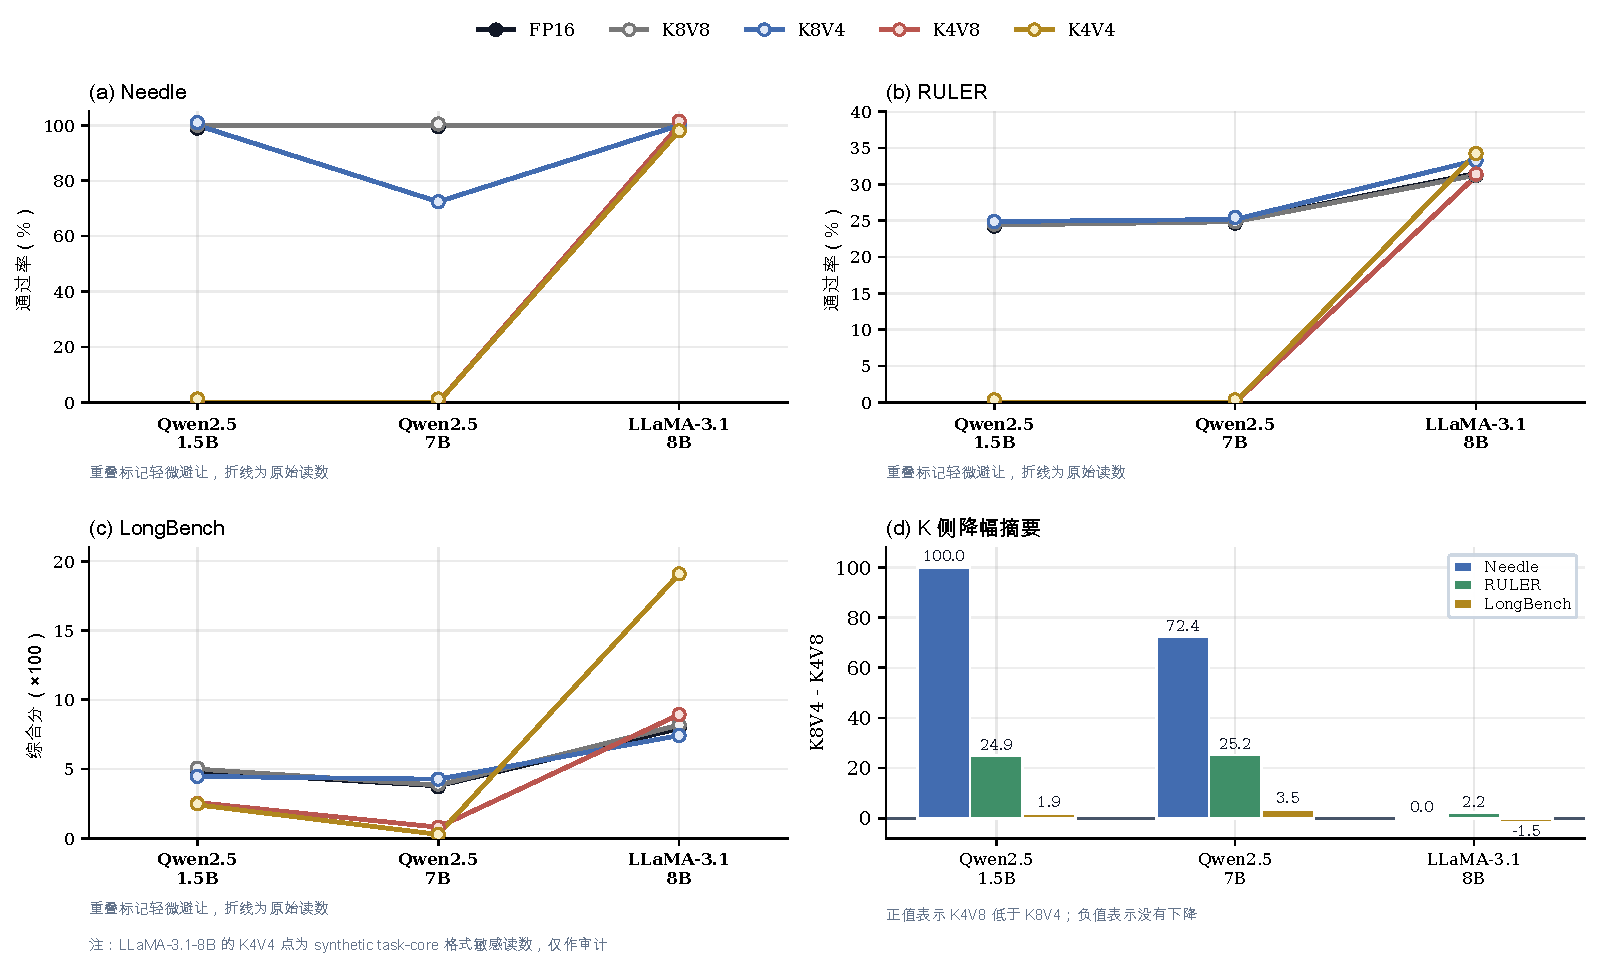
\includegraphics[width=\linewidth]{figures/ch4/fig_ch4_01_kv_ruler32.pdf}
  \caption{K/V 角色敏感性的跨指标诊断图。子图（a）--（c）分别在 Needle、RULER 与 LongBench-style 指标上比较主要位宽布局；横轴为模型，折线表示不同位宽布局的原始分数。为避免完全重叠，部分标记做微小纵向避让，但折线仍连接原始读数。子图（d）汇总 \texttt{K4V8} 相对 \texttt{K8V4} 的下降幅度。Qwen 系列在 \texttt{K4V8}/\texttt{K4V4} 下出现稳定 cliff，而 LLaMA-3.1-8B 不呈现同强度坍塌，因此该现象应理解为受架构调制的 Key-side low-bit 敏感性，而不是所有模型同强度规律。}
  \label{fig:ch4-kv-ruler32}
  \label{fig:kv-ablation-summary-ruler}
\end{figure}

图~\ref{fig:ch4-kv-ruler32} 将 Needle、RULER 与 LongBench-style 放到同一位宽布局矩阵中。Qwen2.5-1.5B 与 Qwen2.5-7B 的共同模式是：\texttt{K8V8} 与 \texttt{K8V4} 大体保持可用，而 \texttt{K4V8} 和 \texttt{K4V4} 在 Needle 与 RULER 上直接跌入 cliff，LongBench-style 也同步下降。LLaMA-3.1-8B 则不表现出同强度 cliff：\texttt{K4V8} 在三类指标上仍接近高精度路径，\texttt{K4V4} 在 Needle 与 RULER 上也未出现同幅度坍塌；其 LongBench-style 高读数作为 synthetic task-core 的格式敏感结果保留在图中，但不用于支持“\texttt{K4V4} 优于 \texttt{FP16}”这一判断。由此，本图支持的结论不是“所有模型都会同样 Key 崩”，而是：4bit Key 扰动在 Qwen 系列上会稳定触发行为崩塌，但其强度受到模型族、规模与 $H_{kv}$ 等架构因素调制。

\begin{figure}[t]
  \centering
  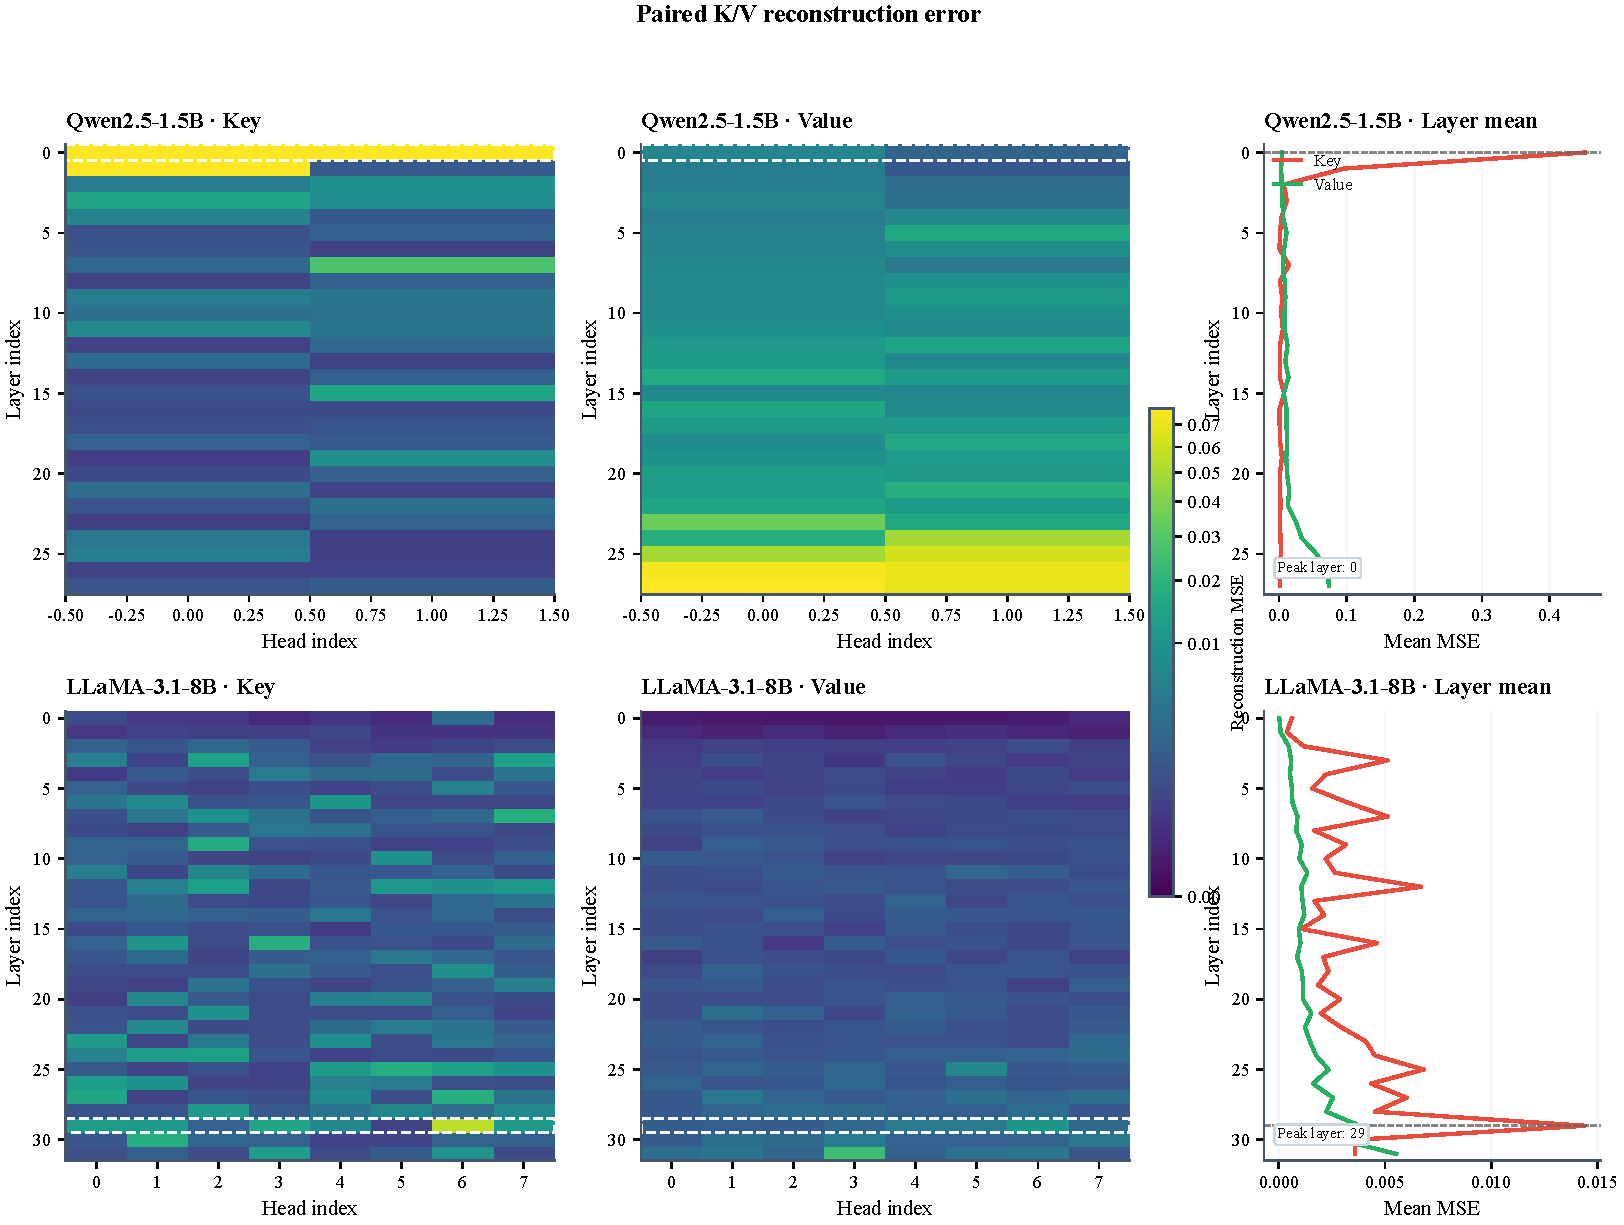
\includegraphics[width=\linewidth]{figures/ch4/fig_ch4_02_kv_error_heatmap.pdf}
  \caption{Qwen2.5-1.5B 与 LLaMA-3.1-8B 的配对 K/V 重建误差热力图（MixedKV，\texttt{K@INT8+V@INT4}，32K 上下文）。上排为 Qwen2.5-1.5B，下排为 LLaMA-3.1-8B；左两列分别为 Key 与 Value 的逐层逐头重建误差，右列为逐层平均误差曲线。统一色标显示：相较于 Qwen2.5-1.5B，LLaMA-3.1-8B 的高误差层段更集中、整体误差更低，与其更强的噪声稀释能力一致。}
  \label{fig:ch4-kv-error-heatmap}
\end{figure}

图~\ref{fig:ch4-kv-error-heatmap} 从误差结构侧补充了这种架构依附性。配对热力图显示，在 \texttt{MixedKV} 配置下，Qwen2.5-1.5B 的高误差层段更早、更分散，而 LLaMA-3.1-8B 的误差峰值则更集中于后部层段，整体量级也更低。这张图不是 attention-KL 主指标的替代物，但它支持了与表~\ref{tab:ch4-kv-multitask} 同方向的解释：在更高 $H_{kv}$ 与更平滑的架构条件下，Key 量化噪声更不容易被放大成检索崩塌。

最后，再用一条补充性扩展把这一结论从小模型与中等规模模型延伸到更大模型。在 Qwen2.5-14B 上，保持 Key 为高精度的 \texttt{K16V4} 可将 PPL 从 full \texttt{INT4} 的 5.040 恢复到 4.709，即恢复约 93\% 的退化；相对地，保持 Value 为高精度的 \texttt{K4V16} 仅能恢复到 4.813，恢复率约 64\%。这表明在当前 14B 的补充对比中，保持 Key 为高精度能够带来更大的恢复幅度。至此，本节可以把诊断结论压成一句设计启示：在本文考察的 low-bit 场景中，真正首先触发行为崩塌的是 Key 精度下降；而 \texttt{MixedKV} 的恢复则表明，低比特路径的首要动作不是继续平均压缩 K/V，而是优先保护 Key，并在此基础上升级量化格式。

\subsection{INT4-RoleAlign 与 KIVI-style 的跨模型对比}
\label{subsec:ch4-rolealign-kivi}
\label{subsec:exp-int4-cross-model}
\label{sec:exp-rolealign}

如果第~\ref{subsec:ch4-kv-diagnosis}~节的结论成立，那么下一步就不应再在对称 \texttt{INT4} 的参数空间中继续调参，而应进入 role-aware 非对称格式空间。在这一空间内，本文采用的 \texttt{INT4-RoleAlign} 与 \texttt{KIVI-style} 共享相同的缓存格式，即 \texttt{per-channel K + per-token V}；因此，本小节比较的是同一量化格式下两种校准实例化方式。二者在设计层面的差异已在第三章第~\ref{subsec:ch3-rolealign-vs-kivi}~节中说明，这里不再重复放置设计差异表，而是集中报告同格式条件下的经验结果，并在表注中区分完整配对比较与仅用于界定适用范围的行。

\begin{table}[t]
  \centering
  \caption{INT4-RoleAlign 与 KIVI-style 的跨模型主对比}
  \label{tab:ch4-rolealign-kivi}
  \label{tab:t2-int4-kivi}
  {%
  \footnotesize
  \setlength{\tabcolsep}{4pt}
  \renewcommand{\arraystretch}{1.05}
  \begin{tabular}{lccccccc}
    \toprule
    模型 & $H_{kv}$ & FP16 PPL & KIVI-style PPL & RoleAlign PPL & $\Delta$PPL & KIVI Needle & RoleAlign Needle \\
    \midrule
    Qwen2.5-1.5B & 2 & 9.31 & 10.43 & 10.58 & +0.15 & 100/100\% & 100/100\% \\
    Qwen2.5-7B   & 4 & 7.14 & 7.53  & 7.58  & +0.05 & 100/100\% & 100/100\% \\
    LLaMA-3.1-8B & 8 & 6.73 & 6.90  & 6.90  & +0.00 & 100/100\% & 100/100\% \\
    Qwen2.5-14B  & 8 & 4.68 & --    & 5.04  & --    & --         & 100/100\% \\
    \bottomrule
  \end{tabular}

  \vspace{0.35em}
  \begin{minipage}{0.94\linewidth}
    \footnotesize
    注：两者共享 \texttt{per-channel K + per-token V} 非对称格式，唯一差异是校准理念：\texttt{RoleAlign} 采用离线 role-aware calibration，其中 K-path 以 attention-distribution KL 为主代理，并在离线搜索纪律下确定参数，V-path 由独立输出扰动代理主导；\texttt{KIVI-style} 使用运行时 \texttt{absmax/min}。Needle 列中的“100/100”表示 \texttt{Needle-single-retrieval} 与 \texttt{MK-NIAH-2} 两类检索同时恢复到 100\%。Qwen2.5-1.5B、Qwen2.5-7B 与 LLaMA-3.1-8B 构成当前正文中的完整配对对比；Qwen2.5-14B 当前仅提供 RoleAlign 结果，因此该行主要用于界定比较范围，而不参与配对差异判断。为保持与现有结果资产的一致性，1.5B 行采用当前主协议下的重跑结果，7B/8B/14B 行采用同格式、同指标定义下的既有对比结果。
  \end{minipage}
  }
\end{table}

表~\ref{tab:ch4-rolealign-kivi} 显示，在共享非对称格式的前提下，\texttt{INT4-RoleAlign} 与 \texttt{KIVI-style} 的经验差距并不是一边倒式的大缺口。在当前可直接配对的 1.5B、7B 与 8B 三个模型上，RoleAlign 相对 KIVI-style 的 PPL 差距分别为 $+0.15$、$+0.05$ 与 $+0.00$；Needle 则在三者上都恢复到 100/100\%。14B 的 RoleAlign 行只用于说明该格式在更大模型上的当前覆盖范围，不参与差异判断。这一结果首先说明：\textbf{决定低比特检索恢复的关键首先是角色感知非对称格式本身。} 一旦从对称 per-group 升级到 \texttt{per-channel K + per-token V}，低比特路径就已经从“完全崩塌”转回“可用状态”。在此基础上，校准理念的差异更多体现在实例化方式，而不是大幅拉开质量缺口。

离线行为引导校准的独立价值主要体现在组织方式而非一边倒的经验差距。当前证据支持的更稳解释是：在同格式条件下，\texttt{RoleAlign} 的优势不在于把 \texttt{KIVI-style} 远远甩开，而在于它把低比特路径组织成了一条\textbf{可固化、可审计、可扩展}的实例化路径。\texttt{KIVI-style} 依赖运行时 \texttt{absmax/min} 重算 scale，\texttt{RoleAlign} 则将 K-path 与 V-path 的分路校准结果固化为离线校准结果；也正因为如此，\texttt{RoleAlign} 才能自然延伸到后续的行为引导分配器，而不是停留在一个只做运行时统计的缓存格式基线上。本小节支持的是“格式是一阶、离线校准是二阶组织增益”的当前判断。

至此，低比特恢复问题已经得到回答：第~\ref{subsec:ch4-int4-cliff}~节说明行为引导原则在对称 \texttt{INT4} 上首先遭遇架构依附性的阶跃失效；第~\ref{subsec:ch4-kv-diagnosis}~节进一步表明，该失效主要由 Key 侧精度下降触发，而 \texttt{MixedKV} 的恢复指向“Key 优先保护”与角色感知格式升级；最后，本小节说明在共享非对称格式的公平设置下，\texttt{INT4-RoleAlign} 可以把这一路径恢复为一个可审计、可扩展的低比特实例。接下来的问题，不再是低比特路径能否被恢复，而是恢复后的行为敏感度画像能否进一步支撑跨模型预算分配，并读出稳定的策略适用区间结构。

\section{跨模型预算分配与策略适用区间图谱}
\label{sec:ch4-rq3}
\label{sec:exp-cross-model}
\label{sec:exp-per-model}

第~\ref{sec:ch4-rq2} 节已经确认，低比特路径可以在角色感知非对称格式下被恢复。本节进一步回答跨模型预算分配问题：由行为引导校准产出的敏感度画像，是否能够支撑跨模型预算分配，并揭示稳定的策略适用区间结构。本节的目标不是寻找一个跨模型的单一普适最优策略，而是把分配器结果从若干跑分表提升为一张可命名的适用区间图谱。

为避免将 allocator 结果误读为单一策略排名，本节首先在同量级 INT4 预算带内给出跨模型主表，再通过四个典型剖面概括不同模型上的结构落点。这里所谓“策略适用区间”，指的是在给定模型族、规模与任务组合下，某类 allocator 策略更容易落在该模型的高性能区间，而不是在严格同预算条件下已经被形式化证明更优。

\subsection{同量级预算下的跨模型主表}
\label{subsec:ch4-regime-main}

本节先明确比较口径。表~\ref{tab:ch4-regime-main} 报告的是同量级 INT4 预算带内的结构读数，而不是严格同显存的 $\pm 3\%$ 对照。当前各 allocator 策略的平均位宽大致落在 $4.5\text{--}5.0$ bit 带内，而 uniform \texttt{INT4} 对应 $\bar b = 4.0$ bit，因此这里的主要作用，是回答“在同一数量级预算内，不同分配风格会在不同模型上落到哪里”，而不是回答“在严格同预算下谁被形式化证明更优”。这一边界同时也是本节与未来严格同预算比较的分界线。

\begin{table}[t]
  \centering
  \caption{同量级 INT4 预算带内的跨模型主表}
  \label{tab:ch4-regime-main}
  \label{tab:t3-cross-model-main}
  {%
  \footnotesize
  \setlength{\tabcolsep}{4pt}
  \renewcommand{\arraystretch}{1.05}
  \begin{tabular}{llcccc}
    \toprule
    模型 & 任务/汇总 & Uniform INT4 & BA-k & Heuristic-k & BA-AutoK \\
    \midrule
    \multirow{4}{*}{Qwen2.5-3B ($H_{kv}=2$)}
      & NarrativeQA (F1)    & 4.33 & \textbf{7.17} & 3.08 & 6.48 \\
      & HotpotQA (F1)       & 2.38 & 4.73 & 1.39 & \textbf{4.89} \\
      & GovReport (Rouge-L) & 5.77 & 8.81 & 5.96 & \textbf{8.90} \\
      & Mean                & 4.16 & \textbf{6.90} & 3.48 & 6.75 \\
    \midrule
    \multirow{4}{*}{LLaMA-3.1-8B ($H_{kv}=8$)}
      & NarrativeQA (F1)    & 10.24 & \textbf{11.14} & 10.47 & 10.74 \\
      & HotpotQA (F1)       & 6.73  & \textbf{7.88}  & 5.68  & 7.57 \\
      & GovReport (Rouge-L) & 9.24  & 9.54 & 9.47 & \textbf{9.75} \\
      & Mean                & 8.74  & \textbf{9.52} & 8.54 & 9.35 \\
    \midrule
    \multirow{4}{*}{Qwen2.5-14B ($H_{kv}=8$)}
      & NarrativeQA (F1)    & \textbf{7.05} & 6.67 & 6.83 & 6.80 \\
      & HotpotQA (F1)       & \textbf{5.57} & 5.49 & 5.40 & 5.39 \\
      & GovReport (Rouge-L) & 9.09 & 8.95 & 9.03 & \textbf{9.27} \\
      & Mean                & \textbf{7.23} & 7.04 & 7.09 & 7.15 \\
    \midrule
    \multirow{4}{*}{Mistral-7B-v0.3 ($H_{kv}=8$)}
      & NarrativeQA (F1)    & 15.55 & 15.71 & \textbf{17.11} & 16.26 \\
      & HotpotQA (F1)       & 17.81 & 17.78 & 17.84 & \textbf{19.08} \\
      & GovReport (Rouge-L) & 8.70  & 8.66  & 8.86 & \textbf{8.96} \\
      & Mean                & 14.02 & 14.05 & 14.60 & \textbf{14.76} \\
    \bottomrule
  \end{tabular}

  \vspace{0.35em}
  \begin{minipage}{0.94\linewidth}
    \footnotesize
    注：本表报告的是同量级 INT4 预算带内的跨模型读数，而不是严格同预算比较。各模型的 best-$k$ 动态选择为：Qwen2.5-3B 用 $k=1$，LLaMA-3.1-8B 用 $k=11$，Qwen2.5-14B 用 $k=7$，Mistral-7B 用 $k=3$；AutoK 的覆盖阈值在 14B 上为 90\%，其余模型为 80\%。Uniform 指所有层 K/V 统一采用 INT4；BA-k 指 behavior-guided allocator 保护 top-$k$ 高敏感层；Heuristic-k 指等距位置启发式保护；BA-AutoK 指根据覆盖率准则自动确定保护层数的 behavior-guided allocator。
  \end{minipage}
  }
\end{table}

表~\ref{tab:ch4-regime-main} 的核心信息不是“哪一列整体最高”，而是四个模型的最佳策略家族并不一致：Qwen2.5-3B 的三任务均值最优落在 BA-k1，LLaMA-3.1-8B 的三任务均值最优落在 BA-k11，Qwen2.5-14B 的最高均值落在 Uniform，而 Mistral-7B 的三任务均值最优则落在 BA-AutoK。这些差异并不能仅凭与敏感度画像的对应关系单独成立；它们首先需要与图~\ref{fig:ch4-autok-protection} 中的保护层结构相互印证，而图~\ref{fig:ch4-regime-heatmap} 则把这种异质性整理为后续四个模型剖面的阅读路线图。

\begin{figure}[t]
  \centering
  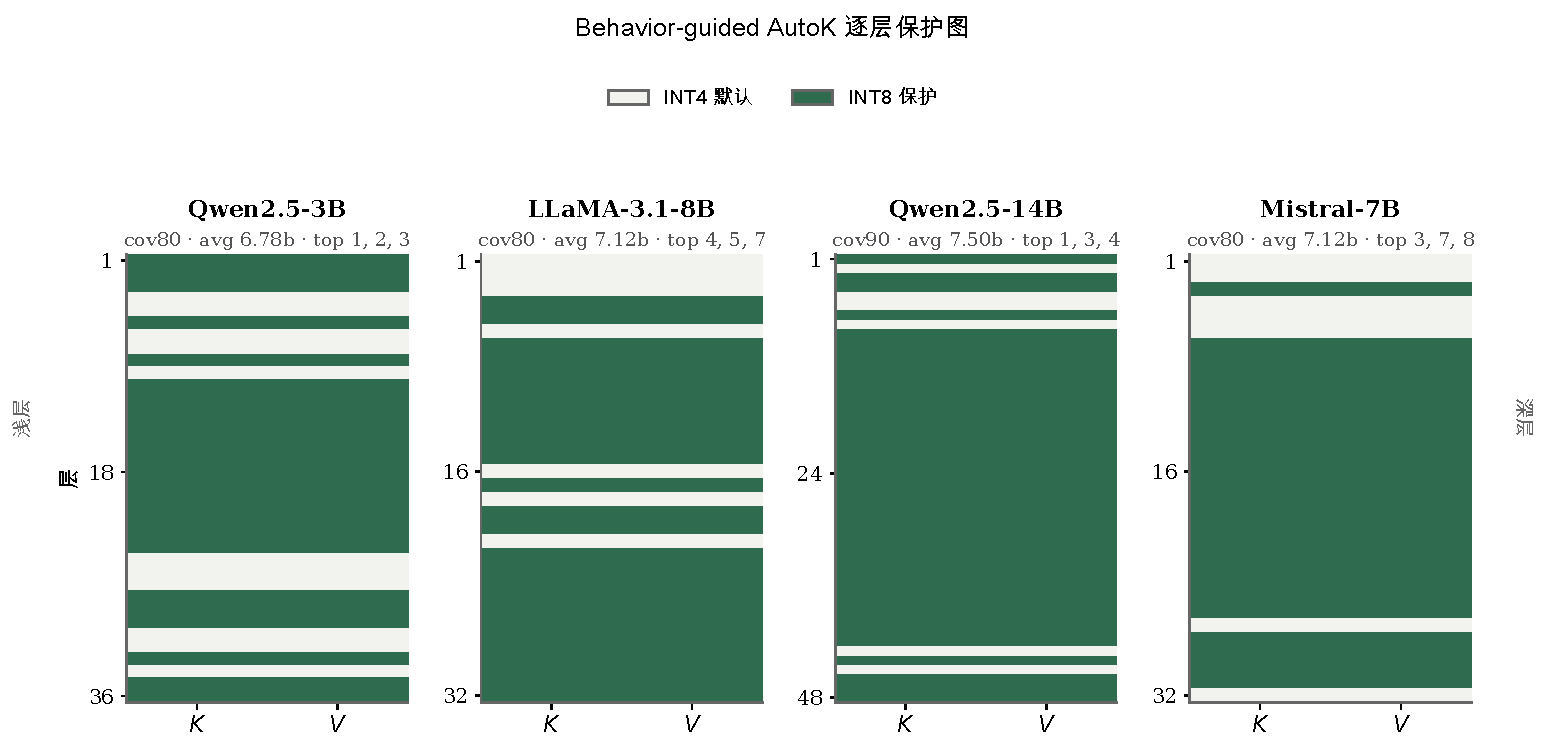
\includegraphics[width=\linewidth]{figures/ch4/fig_ch4_03_autok_protection_map.pdf}
  \caption{Behavior-guided AutoK 的逐层保护决策。四个子图分别对应 Qwen2.5-3B、LLaMA-3.1-8B、Qwen2.5-14B 与 Mistral-7B，展示同一 coverage 规则下各模型的保护层结构。该图将跨模型主表背后的 sensitivity shape 直接可视化。}
  \label{fig:ch4-autok-protection}
  \label{fig:sensitivity-heatmap}
\end{figure}

图~\ref{fig:ch4-autok-protection} 把这种结构差异直接可视化。Qwen2.5-3B 的保护层明显前移并集中于最早层，说明其 sensitivity profile 呈现典型的 early-layer bottleneck；LLaMA-3.1-8B 与 Mistral-7B 则呈现中层簇集，说明在中等规模与特定家族上，真正关键的层已经不是单一首层，而是一簇相邻的高敏感层；Qwen2.5-14B 则近乎铺满全深度，表现为广泛铺展的 profile，说明大模型的行为敏感度已经显著弥散化。于是，“不同模型最优项不同”不再只是表格现象，而与 sensitivity structure 的差异相互印证。

\begin{figure}[t]
  \centering
  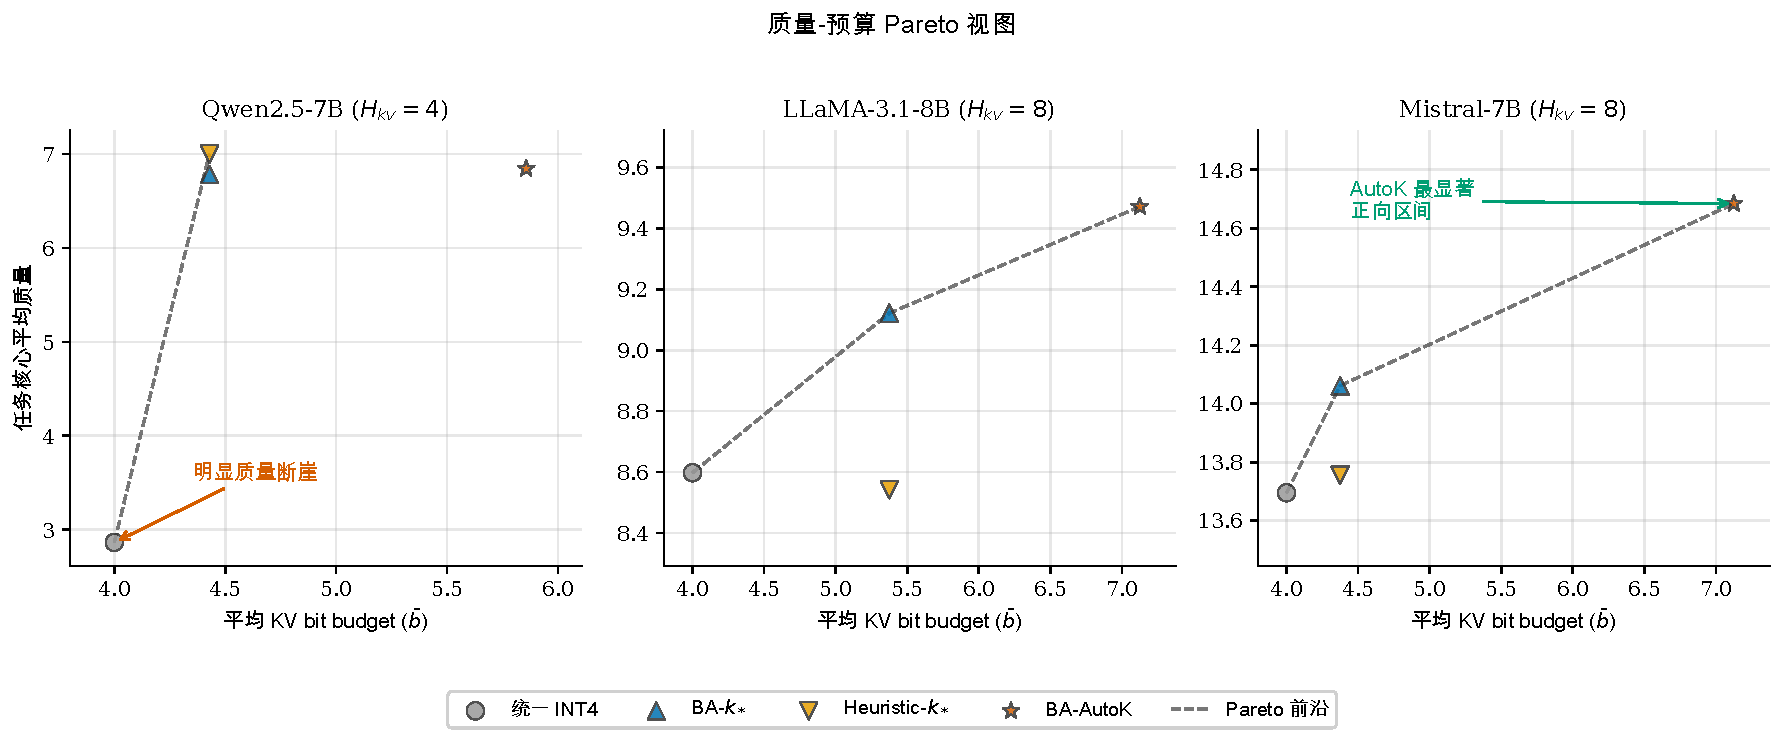
\includegraphics[width=\linewidth]{figures/ch4/fig_ch4_04_pareto_budget_quality.pdf}
  \caption{质量-预算 Pareto 视图。三个子图分别对应 Qwen2.5-7B、LLaMA-3.1-8B 与 Mistral-7B；横轴为平均 KV bit budget，纵轴为任务核心平均质量。该图用于可视化同量级 INT4 预算带下不同策略家族的局部几何关系，而不是严格的同预算比较。}
  \label{fig:ch4-pareto}
  \label{fig:t7-pareto}
\end{figure}

\begin{figure}[t]
  \centering
  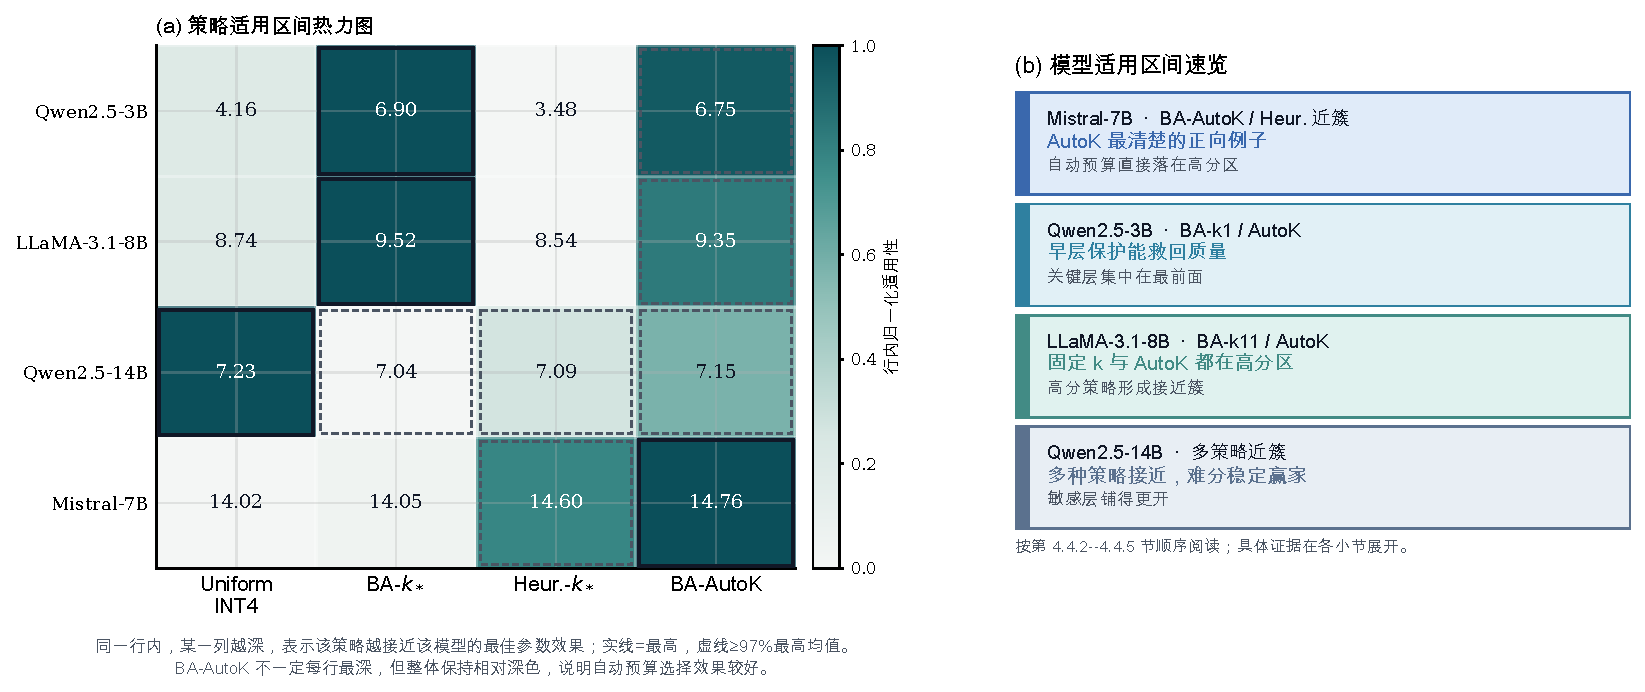
\includegraphics[width=\linewidth]{figures/ch4/fig_ch4_05_regime_heatmap.pdf}
  \caption{跨模型策略适用区间与模型适用区间速览。左图展示各模型在四类策略家族下的任务核心平均质量；同一模型所在行内，某一列颜色越深表示该策略越接近该模型的高性能区间，但颜色不表示跨模型绝对质量可比。BA-AutoK 列虽然并非每行最深，但整体处于相对深色区间，因此可视为效果较好的自动预算候选。实线边框标出每行最高落点，虚线边框标出达到该行最高三任务均值 $97\%$ 以上的近簇。右图按后文模型分析顺序列出四类待展开结构类型，作为第 4.4.2--4.4.5 节的阅读路线图。}
  \label{fig:ch4-regime-heatmap}
\end{figure}

图~\ref{fig:ch4-pareto} 与图~\ref{fig:ch4-regime-heatmap} 进一步把主表读成适用区间，而不是简单排名。Pareto 图说明同量级预算带内确实存在清晰的质量--预算局部几何：Mistral-7B 上 AutoK 区域最为突出，LLaMA-3.1-8B 上几种高性能策略形成近 Pareto 的局部簇；Qwen2.5-7B 的补充结果只作为 uniform policy 质量断崖的旁证，不进入后文四个模型剖面节。合并后的适用区间图则承担两层作用：左图把四模型压缩成“每行一个高性能落点”的速览图，右图按 Mistral-7B、Qwen2.5-3B、LLaMA-3.1-8B 与 Qwen2.5-14B 的后文顺序提示四个待展开结构类型，而不是在本小节完成证明。值得注意的是，position-based heuristic 在多个区间内与 behavior-guided 选中集合发生重合；这一强基线现象的结构性含义，将在第 4.6.3 节中进一步讨论。

\subsection{Mistral-7B：AutoK 的单模型支持证据}
\label{subsec:ch4-profile-mistral}
\label{subsec:exp-per-model-mistral}

Mistral-7B 被单独列出，是因为它提供了当前最清晰的 AutoK 单模型支持证据。该剖面的价值不在于证明“AutoK 普适最优”，而在于回答一个更窄也更重要的问题：当敏感度画像本身具有可压缩的中层簇集结构时，覆盖度预算建议能否读出层间结构。

\begin{table}[t]
  \centering
  \caption{典型剖面表 A：Mistral-7B 与 Qwen2.5-3B}
  \label{tab:ch4-profile-a}
  \label{tab:t4-mistral-autok}
  \label{tab:t5-3b-early-layer}
  {%
  \footnotesize
  \setlength{\tabcolsep}{4pt}
  \renewcommand{\arraystretch}{1.05}
  \begin{tabular}{lcccccc}
    \toprule
    \multicolumn{7}{l}{\textbf{Panel A. Mistral-7B：AutoK 的单模型支持证据}} \\
    \midrule
    任务 & Uniform & BA-k3 & Heuristic-k3 & \makecell[c]{BA-AutoK\\(80\%)} & 最优项 & 备注 \\
    \midrule
    NarrativeQA (F1)    & 15.55 & 15.71 & \textbf{17.11} & 16.26 & Heur-k3 & \\
    HotpotQA (F1)       & 17.81 & 17.78 & 17.84 & \textbf{19.08} & AutoK & \\
    GovReport (Rouge-L) & 8.70  & 8.66  & 8.86 & \textbf{8.96}  & AutoK & \\
    DuReader (Rouge-L)  & 7.35  & 8.64  & 7.97 & \textbf{11.62} & AutoK & 增益最大 \\
    LCC (EditSim)       & 21.38 & \textbf{22.10} & 20.30 & 19.77 & BA-k3 & \\
    Mean                & 14.16 & 14.58 & 14.42 & \textbf{15.14} & AutoK & 5-task mean \\
    \midrule
    \multicolumn{7}{l}{\textbf{Panel B. Qwen2.5-3B：早层保护有效区间}} \\
    \midrule
    任务 & Uniform & BA-k1 & Heuristic-k1 & \makecell[c]{BA-AutoK\\(80\%)} & Quality $\Delta$ & 备注 \\
    \midrule
    NarrativeQA (F1)    & 4.33 & \textbf{7.17} & 3.08 & 6.48 & +4.09 & 提升 \\
    HotpotQA (F1)       & 2.38 & 4.73 & 1.39 & \textbf{4.89} & +3.33 & 提升 \\
    GovReport (Rouge-L) & 5.77 & 8.81 & 5.96 & \textbf{8.90} & +2.85 & 提升 \\
    Mean                & 4.16 & \textbf{6.90} & 3.48 & 6.75 & +3.42 & 差距最大 \\
    \bottomrule
  \end{tabular}

  \vspace{0.35em}
  \begin{minipage}{0.94\linewidth}
    \footnotesize
    注：Panel A 来自 Mistral-7B-v0.3 的 5-task 扩展剖面；Panel B 来自 Qwen2.5-3B 的 3-task task-core 剖面。Mistral 的 AutoK 覆盖阈值为 80\%；Qwen2.5-3B 的 behavior-guided best-$k$ 为 $k=1$。本表由第 4.4.2 节与第 4.4.3 节共用，并以双剖面块形式组织。
  \end{minipage}
  }
\end{table}

表~\ref{tab:ch4-profile-a} 的 Panel A 显示，BA-AutoK 在 Mistral-7B 的五个任务中有三个任务给出最高读数，并取得最高平均值。最明显的差异来自 DuReader：BA-AutoK 达到 11.62，而 Heuristic-k3 为 7.97，差距达到 3.6 分；同时，它在 HotpotQA 与 GovReport 上也给出最优读数。由于这些增益分散在多个任务上，而不是由单一异常任务造成，因此它们支持一种基于覆盖率的正向解释，而不只是单个数据集上的偶然波动。

这一优势与图~\ref{fig:ch4-autok-protection} 中的敏感度画像是一致的。Mistral-7B 的重点保护层落在中前层簇集，且 80\% 覆盖阈值选出的保护范围与这种簇集结构相吻合，因此 AutoK 在这里并非偶然获得更好的预算，而是与覆盖率预算建议器所捕捉到的层间结构保持一致。于是，Mistral-7B 在本文中承担的不是“AutoK 跨设置最优”的证明，而是“当画像具有可压缩簇集结构时，覆盖率预算建议器可以给出清晰正向信号”的单模型实例。

\subsection{Qwen2.5-3B：早层保护有效区间}
\label{subsec:ch4-profile-qwen3b}
\label{subsec:exp-per-model-3b}

Qwen2.5-3B 则承担了全文最清晰的行为引导策略与位置启发式差距剖面。它之所以单列，不是因为总体分数最高，而是因为它揭示了一类更窄但更重要的适用区间：当行为敏感度高度集中于最早几层时，保护正确的第一层会产生质量提升，而位置启发式若把预算投向“看起来更居中”的层，可能难以覆盖关键瓶颈位置。

表~\ref{tab:ch4-profile-a} 的 Panel B 给出了这一点的主要数字支撑。对 BA-k1 与 Heuristic-k1 的直接比较表明，BA-k1 在 NarrativeQA 上高出 4.09 分，在 HotpotQA 上高出 3.33 分，在 GovReport 上高出 2.85 分，平均差距达到 3.42 分。这里最关键的不是增益的绝对量，而是增益的语义：这些差距对应于从低质量区间进入可用区间，因此应被读作早层保护带来的质量提升。

这一恢复性收益与图~\ref{fig:ch4-autok-protection} 的 3B 结构读数一致。Qwen2.5-3B 的敏感度画像明显前移，top protected layers 集中在最早层；BA-k1 保护的是 layer 0，而 Heuristic-k1 的单层保护则落在中层，因而偏离瓶颈层。3B 并不是在证明“小模型总该用 BA-k1”，而是在定义一种更精确的适用区间：当行为敏感度在最早几层高度集中时，位置启发式可能偏离关键层，而行为引导保护可以产生恢复性收益。

\subsection{LLaMA-3.1-8B：中等规模共识区间}
\label{subsec:ch4-profile-llama8b}

LLaMA-3.1-8B 是当前主线中的一个重要模型案例。跨模型主表已经显示出足够清晰的结构信号：最佳平均值落在 BA-k11，同时 BA-AutoK 与其它高性能策略距离并不远。因此，本节将这行结果展开为一个可单独讨论的结构区间。

\begin{table}[t]
  \centering
  \caption{典型剖面表 B：LLaMA-3.1-8B 与 Qwen2.5-14B}
  \label{tab:ch4-profile-b}
  \label{tab:t6-14b-toptier}
  {%
  \footnotesize
  \setlength{\tabcolsep}{4pt}
  \renewcommand{\arraystretch}{1.05}
  \begin{tabular}{lcccccc}
    \toprule
    \multicolumn{7}{l}{\textbf{Panel A. LLaMA-3.1-8B：中等规模共识区间}} \\
    \midrule
    任务 & Uniform & BA-k11 & Heuristic-k11 & \makecell[c]{BA-AutoK\\(80\%)} & 最优项 & 备注 \\
    \midrule
    NarrativeQA (F1)    & 10.24 & \textbf{11.14} & 10.47 & 10.74 & BA-k11 & \\
    HotpotQA (F1)       & 6.73  & \textbf{7.88}  & 5.68  & 7.57  & BA-k11 & \\
    GovReport (Rouge-L) & 9.24  & 9.54 & 9.47 & \textbf{9.75} & AutoK & \\
    Mean                & 8.74  & \textbf{9.52} & 8.54 & 9.35 & BA-k11 & 共识高性能区间 \\
    \midrule
    \multicolumn{7}{l}{\textbf{Panel B. Qwen2.5-14B：高性能簇共存而无稳定最优}} \\
    \midrule
    任务 & Uniform & BA-k7 & Heuristic-k7 & \makecell[c]{BA-AutoK\\(90\%)} & $gap_{\mathrm{rel}}$ & 备注 \\
    \midrule
    NarrativeQA (F1)    & \textbf{7.05} & 6.67 & 6.83 & 6.80 & 3.55\% & top-3 聚簇 \\
    HotpotQA (F1)       & \textbf{5.57} & 5.49 & 5.40 & 5.39 & 3.05\% & top-3 聚簇 \\
    GovReport (Rouge-L) & 9.09 & 8.95 & 9.03 & \textbf{9.27} & 2.59\% & top-3 聚簇 \\
    Mean                & \textbf{7.23} & 7.04 & 7.09 & 7.15 & 3.06\% & max $\approx$ 3.5\% \\
    \bottomrule
  \end{tabular}

  \vspace{0.35em}
  \begin{minipage}{0.94\linewidth}
    \footnotesize
    注：Panel A 展示 LLaMA-3.1-8B 的中等规模共识区间；Panel B 展示 Qwen2.5-14B 的高性能策略簇。Qwen2.5-14B 的 \mbox{$gap_{\mathrm{rel}}(t)=(top1(t)-top3(t))/top1(t)$} 最大约 3.5\%，平均约 3.0\%。在当前统计功效下，14B 的高性能策略更适合解释为近似不可分辨的策略簇，而不是稳定单一最优。
  \end{minipage}
  }
\end{table}

表~\ref{tab:ch4-profile-b} 的 Panel A 表明，LLaMA-3.1-8B 的确存在一个较明确的 BA-k11 结构落点：NarrativeQA 与 HotpotQA 上 BA-k11 都给出最优读数，GovReport 上则由 BA-AutoK 略占优势，最终平均值由 BA-k11 取得最优。这里最值得强调的不是单点策略相对其它策略形成绝对优势，而是它与 BA-AutoK 之间的差距非常有限；再结合图~\ref{fig:ch4-pareto} 中近 Pareto 的局部几何关系，更合理的读法是：LLaMA-3.1-8B 所代表的，是一个 \emph{共识高性能区间}，而不是单点独占。

这一命名与其敏感度画像形状也是一致的。与 Qwen2.5-3B 的尖锐前层集中不同，LLaMA-3.1-8B 的最佳保护范围已经扩展到更广的中层簇集，best-$k=11$ 本身就意味着“单点保护”不再是合理抽象；但与此同时，它又不像 Qwen2.5-14B 那样弥散到几乎全深度广泛铺展。因此，LLaMA-3.1-8B 最适合被命名为 \textbf{中等规模共识区间}：存在一个相对稳定的 BA-k 结构落点，但其它高性能策略并未远离。它在本文中还承担一个更克制的对照角色：由于其 $H_{kv}=8$ 设置与较平滑的分配器响应同时出现，我们可以把它当作 GQA 架构稳健性的补充剖面，但不能把它升级为“更高 $H_{kv}$ 必然导向更优策略”的强结论。

\subsection{Qwen2.5-14B：高性能簇共存而无稳定最优}
\label{subsec:ch4-profile-qwen14b}
\label{subsec:exp-per-model-14b}

Qwen2.5-14B 提供的是这张适用区间图谱中的边界剖面：并非每个模型都会给出清晰最优项。它在跨模型主表中的最高均值落在 Uniform，但这一读数如果被直接概括为“Uniform 最优”，就会弱化 14B 的结构形状。对于这个模型，更关键的事实不是某一策略在平均分上略高，而是几类高性能策略彼此接近，以至于在当前证据下更适合被读成近似持平的策略簇。

表~\ref{tab:ch4-profile-b} 的 Panel B 直接支持这一点。三个任务上四类策略的数值都非常接近，按照 $gap_{\mathrm{rel}}(t)=(top1(t)-top3(t))/top1(t)$ 的定义，NarrativeQA、HotpotQA 与 GovReport 的 top-3 相对 top-1 gap 分别约为 3.55\%、3.05\% 与 2.59\%，平均值约为 3.06\%。这意味着 14B 的 top-3 策略全部位于 top-1 的 3.5\% 相对距离内。基于这些相对差距，更稳的解释不是“Uniform 真正最优”，而是：\textbf{14B 当前呈现出一个高性能策略彼此接近的簇，而不是稳定单一最优。}

这种近似持平的格局与图~\ref{fig:ch4-autok-protection} 的广泛铺展画像是一致的。Qwen2.5-14B 的敏感度画像已经近乎铺满全深度，AutoK 在 48 层中标出 42 个受保护层，说明它不是由少数关键层决定一切的模型。正因为画像本身已经高度弥散，分配器在当前预算区间中的选择顺序只会带来有限边际影响。于是，14B 给这张适用区间图谱的不是一个正面最优项，而是一条更稳的结构结论：\textbf{高性能簇共存而无稳定最优。}

回到图~\ref{fig:ch4-regime-heatmap} 的右图，第 4.4 节的四个模型剖面最终对应四类结构类型：Mistral-7B 提供 AutoK 的单模型支持证据，Qwen2.5-3B 是早层保护有效区间，LLaMA-3.1-8B 是中等规模共识区间，Qwen2.5-14B 则是高性能簇共存而无稳定最优。它们共同构成一张按模型族、规模与任务共同决定的适用区间图谱，而不是“哪个策略全局最好”的排行榜。至此，跨模型预算分配问题已经得到回答：行为敏感度画像不只是校准层的副产物，它还能在同量级预算带内支撑跨模型预算分配，并读出稳定而可命名的结构落点。下一节将不再继续讨论质量适用区间，而转向这些路径在真实推理系统中的时间与显存边界。

\section{部署效率评估}
\label{sec:ch4-deployment}
\label{sec:exp-deployment}

第~\ref{sec:ch4-rq1}--\ref{sec:ch4-rq3} 节已经分别回答了基准保真、low-bit 恢复与跨模型策略图谱。本节转向部署层，考察这些路径在真实推理系统中的时间与显存代价。本节不再重复第三章关于 kernel 设计与离线校准产物的实现细节，而是聚焦一个更务实的问题：\emph{在什么条件下，当前低比特部署路径能够带来部署收益；在什么条件下，其收益会受到限制。}

为此，本节按“入口读数 $\rightarrow$ 长序列放大 $\rightarrow$ 经验边界 $\rightarrow$ 部署建议”的顺序组织。首先，第~\ref{subsec:ch4-tpot-4k}~节给出 4K 序列下的后端路径入口读数，避免把任何后续加速误读为无条件现象；随后，第~\ref{subsec:ch4-tpot-scaling}~节展示长序列下融合路径收益如何随上下文增长而放大；在此基础上，第~\ref{subsec:ch4-crossover}~节将这些单点与单模型结果上升为一条可读出的性能交叉边界；最后，第~\ref{subsec:ch4-kvcache}~节用 \texttt{KV Cache} 显存压缩率与当前硬件约束将系统层结论收束为可执行部署建议。

\subsection{4K 序列下的 TPOT 对比}
\label{subsec:ch4-tpot-4k}

短上下文入口层的读数是部署判断的起点。4K 序列既是常见的部署长度点，也是判断固定 kernel 开销是否已经值得付出的最低长度点。因此，这一小节的目的不是证明融合路径已经普适占优，而是先给出各后端路径在当前硬件与 batch 设定下的入口层读数：哪些模型上 Triton 融合路径仍受固定调度开销影响，哪些模型上它已经开始逼近甚至略微越过参考路径。

\begin{table}[t]
  \centering
  \caption{4K 序列下的 TPOT 对比（生成长度 128，batch size 为 1，NVIDIA H20；单位：ms）}
  \label{tab:ch4-tpot-4k}
  {%
  \footnotesize
  \setlength{\tabcolsep}{4pt}
  \renewcommand{\arraystretch}{1.05}
  \begin{tabular}{lccccccc}
    \toprule
    模型 & $H_{kv}$ & FP16 & \makecell[c]{参考路径\\(INT4)} & KIVI(INT4) & \makecell[c]{Triton 融合路径\\(INT4)} & FlashInfer(INT4) & 最快项 \\
    \midrule
    Qwen2.5-1.5B & 2 & 24.36 & 36.35 & 36.39 & 38.68 & 43.73 & 参考路径 \\
    Qwen2.5-7B   & 4 & 24.82 & 37.61 & 37.41 & 38.76 & 47.07 & KIVI \\
    LLaMA-3.1-8B & 8 & 28.55 & 44.88 & 44.70 & \textbf{44.49} & 51.50 & Triton 融合路径 \\
    Qwen2.5-14B  & 8 & 42.58 & 68.07 & 68.46 & \textbf{67.67} & 85.07 & Triton 融合路径 \\
    \bottomrule
  \end{tabular}

  \vspace{0.35em}
  \begin{minipage}{0.94\linewidth}
    \footnotesize
    注：粗体标注同模型 INT4 后端路径中的最快项。该表作为第 4.5.1 节的入口层对照，不承担显著加速宣称；真正的收益边界需结合后续长序列读数与性能交叉边界共同解释。
  \end{minipage}
  }
\end{table}

表~\ref{tab:ch4-tpot-4k} 给出三类清楚但应被克制解释的现象：
\begin{itemize}[leftmargin=2em,itemsep=2pt,topsep=2pt]
  \item 在 $H_{kv}=2$ 的 Qwen2.5-1.5B 上，Triton 融合路径录得 38.68\,ms，高于参考路径的 36.35\,ms。
  \item 在 $H_{kv}=4$ 的 Qwen2.5-7B 上，Triton 融合路径录得 38.76\,ms，也高于参考路径的 37.61\,ms。
  \item 只有在 $H_{kv}=8$ 的两种模型上，Triton 融合路径才开始成为该模型下最快的 INT4 后端路径。对 LLaMA-3.1-8B 与 Qwen2.5-14B，其 TPOT 分别为 44.49\,ms 与 67.67\,ms。
\end{itemize}
4K 入口层的读数不应被写成“融合路径已经普适占优”；它只是一个前置信号：当 $H_{kv}$ 较小、Grid 规模不足时，Triton 的固定调度开销仍然可见，而在 $H_{kv}=8$ 上，融合路径已开始逼近甚至轻微越过参考路径，但清晰优势仍要到长序列下才能被放大。

\subsection{长序列 TPOT 扩展规律}
\label{subsec:ch4-tpot-scaling}

如果 4K 入口层只是一个“优势可能开始出现”的信号，那么长序列读数才是判断融合路径是否真正有部署价值的关键。这里选择 Qwen2.5-14B 作为主要观察对象，不是因为它在所有设置下都最快，而是因为它在 $H_{kv}=8$ 下已经显现出明确的正向趋势，同时长上下文下 memory traffic 足够重，最适合观察融合路径是否会随着历史 KV 的增长而系统性放大收益。

\begin{table}[t]
  \centering
  \caption{部署边界综合表}
  \label{tab:ch4-deployment-boundary}
  {%
	  \scriptsize
	  \setlength{\tabcolsep}{3.0pt}
	  \renewcommand{\arraystretch}{1.14}
	  \begin{tabularx}{\linewidth}{L{1.82cm}C{0.72cm}C{0.82cm}C{0.82cm}C{0.82cm}C{1.62cm}Y}
	    \toprule
	    \multicolumn{7}{l}{\textbf{Panel A. 14B 长序列 TPOT（生成长度 64，10 次运行，H20；ms）}} \\
	    \midrule
		    执行路径 & 4K & 8K & 16K & 32K & \makecell[c]{$\Delta$ vs.\\参考路径} & 备注 \\
	    \midrule
		    FP16             & 42.28 & 42.81 & 42.64 & 43.13 & -- & baseline \\
		    \makecell[l]{参考路径\\(INT4)} & 68.17 & 86.08 & 119.83 & 190.23 & -- & reference \\
		    \makecell[l]{KIVI\\(INT4)} & 68.07 & 86.02 & 121.49 & 187.82 & -- & runtime baseline \\
		    \makecell[l]{Triton 融合路径\\(INT4)} & 67.73 & 71.53 & 86.56 & 113.16 & \makecell[c]{4K: -0.44\\8K: -14.54\\16K: -33.26\\32K: -77.08} & fused path \\
	    \midrule
		    \multicolumn{7}{l}{\textbf{Panel B. 跨模型性能交叉边界（$\Delta T=T_{\mathrm{Triton}}-T_{\mathrm{ref}}$；ms）}} \\
	    \midrule
	    模型 & $H_{kv}$ & \makecell[c]{$\Delta T$\\4K} & \makecell[c]{$\Delta T$\\8K} & \makecell[c]{$\Delta T$\\16K} & \makecell[c]{$\Delta T$\\32K} & 备注 \\
    \midrule
    Qwen2.5-1.5B & 2 & +1.67 & +4.23 & +9.78 & +15.92 & 始终更慢 \\
    Qwen2.5-7B   & 4 & \makecell[c]{+1.03\\n.s.} & \makecell[c]{+1.56\\n.s.} & \makecell[c]{+0.55\\n.s.} & -4.90 & 32K 交叉 \\
    Qwen2.5-14B  & 8 & \makecell[c]{-0.44\\n.s.} & -14.54 & -33.26 & -77.08 & 8K 起加速 \\
    \bottomrule
  \end{tabularx}

  \vspace{0.35em}
  \begin{minipage}{0.94\linewidth}
    \footnotesize
    注：Panel A 与 Panel B 分别对应第 4.5.2 节与第 4.5.3 节。这里的“性能交叉边界”是经验读数，而不是理论闭式模型；8B vs 14B 的同 $H_{kv}=8$ 控制对比不再单列成表，仅在第 4.5.3 节正文中作为补充段落报告。对 4K 处 $|\Delta T|<2$\,ms 的读数，统一标记为 n.s.，不宣称为显著交叉点。
  \end{minipage}
  }
\end{table}

表~\ref{tab:ch4-deployment-boundary} 的 Panel A 说明，融合路径的部署价值并不是在 4K 就被证明，而是在序列拉长之后才被系统性放大。具体而言，Qwen2.5-14B 上 Triton 融合路径相对参考路径的时间差在 4K 处仅为 -0.44\,ms，可视为噪声范围；但从 8K 开始，这一差值迅速扩大到 -14.54\,ms，在 16K 进一步扩大到 -33.26\,ms，而在 32K 达到 -77.08\,ms，对应约 -17\%、-28\% 与 -40\% 的相对降幅。更重要的是，这个趋势是单调的：优势不是在 4K 就被“看出来”，而是在 8K 之后随历史 KV 变长而持续放大。于是，第 4.5.2 节真正证明的不是“14B 在某个点更快”，而是“当 memory traffic 持续上升时，融合路径的带宽节省可以逐步压过固定调度开销”。

\subsection{性能交叉边界与 GQA 影响}
\label{subsec:ch4-crossover}

如果说第~\ref{subsec:ch4-tpot-4k}~节给出的是入口层读数、第~\ref{subsec:ch4-tpot-scaling}~节给出的是单模型的扩展证据，那么本节的任务就是把这些读数上升成一条可命名的经验边界。这里的“性能交叉边界”严格指经验量 $\Delta T = T_{\mathrm{Triton}} - T_{\mathrm{ref}}$ 的符号变化，不是理论闭式模型，也不是严格因果识别。对 4K 处 $|\Delta T|<2$\,ms 的情况，本文统一视为 \texttt{n.s.}；因此本节真正关心的不是“某个后端路径是否快了 0.4\,ms”，而是它何时稳定进入加速区间，以及这条边界如何随 $H_{kv}$ 与序列长度共同移动。

表~\ref{tab:ch4-deployment-boundary} 的 Panel B 清楚给出三条边界路径。对于 Qwen2.5-1.5B（$H_{kv}=2$），$\Delta T$ 在 4K/8K/16K/32K 上分别为 +1.67 / +4.23 / +9.78 / +15.92\,ms，说明融合路径在全长度下都不划算；对于 Qwen2.5-7B（$H_{kv}=4$），$\Delta T$ 在 4K/8K/16K 仍为正或近似零，直到 32K 才降为 -4.90\,ms，说明交叉点被推迟到更长序列；而对于 Qwen2.5-14B（$H_{kv}=8$），$\Delta T$ 从 8K 起就显著为负，并在更长上下文下持续放大。这条经验边界可以压成一句话：\textbf{$H_{kv}$ 越高，交叉点越早；序列越长，融合路径越占优。}

同 $H_{kv}=8$ 的 8B 与 14B 对照仍然是本节的重要补充证据。LLaMA-3.1-8B 与 Qwen2.5-14B 虽然参数规模相差约 1.75 倍，却共享相同的 $H_{kv}=8$；在 4K 处，两者的交叉幅度高度一致，分别为 -0.39\,ms 与 -0.44\,ms。这支持一种更稳的结构性读法：相较于参数量，$H_{kv}$ 更接近当前交叉边界的主导相关变量。但由于当前模型集合中 $H_{kv}$ 与规模并未被完全独立控制，这里仍只能写成\emph{相关性支持}，而不能上升为严格的因果结论。

因此，部署层真正有用的不是某个后端路径在某个表格里多快几毫秒，而是一条可读出的经验边界：$H_{kv}=2$ 基本落在融合路径不划算区，$H_{kv}=4$ 只有到很长序列才越过边界，$H_{kv}=8$ 则在较早长度点就进入收益区间。部署路径的选择因而不应按模型名字决定，而应按 $H_{kv}$ 与序列长度是否已经越过性能交叉边界决定。

\subsection{KV Cache 显存压缩率与部署建议}
\label{subsec:ch4-kvcache}

速度边界只给出了一半答案。对于长上下文部署而言，低比特路径是否值得采用，还取决于它在缓存存储上的直接收益是否稳定、可预期。为此，本节最后报告 KV Cache 显存压缩率，并在时间边界与硬件约束共同作用下，将系统层结论转写成当前平台上的经验部署建议。本小节只保留一张正式表，部署建议不再单独成表。

\begin{table}[t]
  \centering
  \caption{KV Cache 显存压缩率对比（4K 序列，batch size 为 1，仅统计 KV Cache，占用单位：MB）}
  \label{tab:ch4-kvcache-memory}
  {%
  \footnotesize
  \setlength{\tabcolsep}{4pt}
  \renewcommand{\arraystretch}{1.05}
  \begin{tabular}{lccccc}
    \toprule
    模型 & $H_{kv}$ & FP16 KV Cache & INT4 KV Cache & 压缩率 & 备注 \\
    \midrule
    Qwen2.5-1.5B & 2 & 115.5 & 30.7  & 73.4\% & \\
    Qwen2.5-7B   & 4 & 230.9 & 61.5  & 73.4\% & \\
    LLaMA-3.1-8B & 8 & 527.9 & 140.5 & 73.4\% & \\
    Qwen2.5-14B  & 8 & 791.8 & 210.8 & 73.4\% & \\
    \bottomrule
  \end{tabular}

  \vspace{0.35em}
  \begin{minipage}{0.94\linewidth}
    \footnotesize
    注：本表只统计 KV Cache，占用不包含模型权重与激活峰值；因此它服务于缓存压缩率判断，而不用于替代完整的运行时峰值显存分析。相应部署建议见第 4.5.4 节正文结尾。
  \end{minipage}
  }
\end{table}

表~\ref{tab:ch4-kvcache-memory} 表明，INT4 路径在四个代表性模型上都实现了近乎相同的缓存压缩率：Qwen2.5-1.5B 从 115.5\,MB 压缩到 30.7\,MB，Qwen2.5-7B 从 230.9\,MB 压缩到 61.5\,MB，LLaMA-3.1-8B 从 527.9\,MB 压缩到 140.5\,MB，而 Qwen2.5-14B 从 791.8\,MB 压缩到 210.8\,MB，压缩率均约为 73.4\%。这说明在当前 INT4 路径下，\texttt{KV Cache} 的显存收益是稳定且可预估的；它不是只对某个模型成立的偶然现象。

把这一点与前文的时间边界合起来，就得到一个关键部署判断：INT4 路径带来的显存节省是\emph{稳定收益}，而融合 decode 路径的速度收益是\emph{条件性收益}。因此，部署选择的核心不是“是否压缩”，而是“在既定压缩前提下，何时切到融合后端路径更划算”。在当前 NVIDIA H20 (sm\_90, 130 SM, 98 GB HBM) 平台上，更稳的经验规则是：当 $H_{kv}=8$ 且序列长度达到 \texttt{8K} 及以上时，优先选择 Triton 融合路径；对于 $H_{kv}=4$ 的模型，只有在很长的序列区间（如 \texttt{32K} 附近）才值得切换；当 $H_{kv}=2$ 或序列长度短于 \texttt{8K} 时，优先使用参考路径。这些建议严格限定于当前硬件、当前软件栈与当前后端组合，跨硬件时交叉边界可能移动，不应被写成硬件无关的普适定律。

附录第~\ref{sec:app-efficiency-plots}~节进一步给出 Qwen2.5-1.5B 设置下的 batch 维度容量边界、吞吐与显存扩展读数，用于补充审计本节部署建议的适用范围。

至此，第四章的系统层边界已经被限定清楚：INT4 的 \texttt{KV Cache} 显存收益是稳定的，而 Triton 融合路径的时间收益则取决于 $H_{kv}$ 与序列长度是否已经越过性能交叉边界。下一节不再继续报结果，而转入对这些结果为何呈现出当前形状的机制辨析。

\section{实验结果讨论与效度威胁}
\label{sec:ch4-discussion}
\label{sec:exp-discussion}

第~\ref{sec:ch4-rq1}--\ref{sec:ch4-deployment} 节已经分别回答了基准路径保真、低比特恢复、跨模型策略图谱与部署效率边界。本节据此讨论这些结果的机制含义及适用边界。下文依次讨论 KL 与 MSE 校准目标、\texttt{INT4} 结果的分层机制、heuristic 强基线以及效度威胁。

\subsection{KL 与 MSE 校准目标的规模依赖性机制辨析}
\label{subsec:ch4-disc-kl-mse}

在 \texttt{INT8} 基准路径已经通过第~\ref{subsec:ch4-int8-canonical}~节与第~\ref{subsec:ch4-longbench-official}~节立住之后，读者自然会追问：既然当前主线校准目标写成 KL，为什么这里不是更常见的 MSE 或其它数值重建代理？这个问题不属于第三章的方法定义层，而属于第四章的必要性边界层。第三章第~\ref{sec:ch3-calibration}~节负责回答“为什么 KL 可作为行为代理”；本节要回答的则是：\emph{在什么条件下，这个代理更必要；又在什么条件下，它会与数值代理趋同。}

就本章直接展示的证据而言，更稳的判断不是“KL 永远显著优于 MSE”，而是“KL 的必要性会随位宽压缩强度与模型鲁棒性而变化”：当量化扰动足以改变 attention ranking 时，分布侧代理更重要；当量化扰动已经被模型冗余度、位宽与架构平滑性共同吸收时，KL 与数值代理会趋同。KL 在本文中的角色应理解为\emph{更贴近行为损伤的可操作代理}，而不是跨所有 setting 的统一胜利者。

\begin{table}[t]
  \centering
  \caption{7B 上 KL 与 MSE 校准目标的趋同验证}
  \label{tab:ch4-kl-mse-convergence}
  {%
  \footnotesize
  \setlength{\tabcolsep}{4pt}
  \renewcommand{\arraystretch}{1.05}
  \begin{tabularx}{\linewidth}{YL{1.8cm}L{1.8cm}C{1.15cm}C{1.3cm}C{1.3cm}C{0.8cm}}
    \toprule
    设置 / path & KL-selected params & MSE-selected params & 参数是否趋同 & KL 结果 (PPL) & MSE 结果 (PPL) & $\Delta$ \\
    \midrule
    Qwen2.5-7B-Instruct, INT4-RoleAlign & $(100.0, 99.9)$ & $(100.0, 99.9)$ & 是 & 7.1121 & 7.1121 & 0.00 \\
    \bottomrule
  \end{tabularx}

  \vspace{0.35em}
  \begin{minipage}{0.94\linewidth}
    \footnotesize
    注：本表由附录第~\ref{subsec:app-7b-kl-mse}~节的 7B KL/MSE 溯源结果提炼而来。FP16 基线 PPL 为 6.7097。KL 目标与 MSE 目标分别来自两组冻结的离线校准产物。两者在固定输入序列上的 likelihood 累计结果用 3 个 seeds 验证逐位一致；该表的职责是支撑“规模依赖性边界”，而不是承担新的主结果宣称。
  \end{minipage}
  }
\end{table}

表~\ref{tab:ch4-kl-mse-convergence} 给出了这一问题的最小实证支撑。在 Qwen2.5-7B-Instruct 上，KL 与 MSE 两种目标最终搜索到完全相同的参数组合，即 $k_{\mathrm{pct}}=100.0$、$v_{\mathrm{pct}}=99.9$；两者对应的 \texttt{INT4-RoleAlign} PPL 也完全一致，均为 7.1121。因此，7B 这块证据的关键不是“KL 相比 MSE 带来多大差异”，而是：\textbf{在 7B 这一设定下，KL 与 MSE 已经高度趋同。} 结合附录第~\ref{subsec:app-7b-kl-mse}~节中的补充对照，这一结果提示模型规模与鲁棒性可能调节二者差异，但当前正文证据仍主要支持“趋同已经出现”这一判断。

从机制上看，这一解释是合理的。在更敏感的小模型或更激进的低比特 setting 下，softmax 排序对 Key 误差更脆弱，attention 分布的错位会先于张量范数恶化暴露出来，因此 KL 这类分布代理更有诊断价值；而在较大模型、较高位宽或更平滑的架构上，quantization noise 不足以把 ranking 推离原本稳定区域，于是 KL 与 MSE 选出的参数会逐步收敛。需要强调的是，这仍然是一种\emph{解释性推断}，而不是定理式证明。

因此，本文对 KL 的主张更适合理解为：在 attention ranking 容易被量化噪声改写的场景中，KL 是更贴近行为损伤的可操作代理；而在较稳的规模与较缓和的 setting 下，它可能与 MSE 逐步趋同，而不是始终制造同样大的经验优势。这一表述保留了 behavior-guided 主线，同时避免把校准目标写成普适性 overclaim。

\subsection{INT4 结果的分层机制辨析}
\label{subsec:ch4-disc-int4}
\label{subsec:exp-int4-honest}

\texttt{INT4} 相关结果在前文已经成立；本节讨论的是它们在机制上能被解释到哪一步，而不是重新比较 \texttt{INT4-RoleAlign} 与 \texttt{KIVI-style} 的主表相对表现。这里沿事实层、解释层与开放问题三个层次展开。

从事实层看，在当前主结果覆盖范围内，\texttt{INT4-RoleAlign} 与 \texttt{KIVI-style} 的质量、PPL 与 Needle 差距总体很小。二者共享的角色感知非对称格式是 \texttt{per-channel K + per-token V}。前文表~\ref{tab:ch4-rolealign-kivi} 已经显示，三组完整配对模型上的 PPL 差距都被压在 $|{\Delta}\mathrm{PPL}|\le 0.15$ 范围内，而 Needle 检索共同恢复到 100/100\%。这组事实首先支持的是：\textbf{low-bit 恢复的一阶条件是 role-aware 非对称格式本身。} 一旦从对称 per-group 升级到这一格式，检索行为就已经从“崩塌”回到“可用”；校准理念并未先制造出一边倒的巨大缺口。

从解释层看，当前证据更支持“格式是一阶、校准是二阶组织增益”的判断。所谓“二阶”，不是说离线行为引导校准不重要，而是说它的独立价值主要体现为：它把角色感知格式背后的架构选择解释化、把参数来源固化为可审计的离线校准结果，并为后续分配器留出统一接口。也正因为如此，\texttt{RoleAlign} 在同格式对比中的意义，不应被理解为“在 KIVI-style 之上取得约 0.1 PPL 的相对差异”，而应被理解为“把低比特路径组织成一条可固化、可延伸的框架实例”。这里还必须显式锁定口径，避免旧说法回流：更准确地说，K-path 以 attention-distribution KL 为主代理，并在离线搜索纪律下确定参数，V-path 由独立输出扰动代理主导，两者共享的是校准流程、结果接口与稳健选择纪律。

进一步地，前文 4.3.1–4.3.2 的结果还表明，low-bit cliff 的强度并不只由位宽决定，还受模型族、规模与 $H_{kv}$ 调制。LLaMA-3.1-8B 之所以在对称 \texttt{INT4} 下表现为架构例外，Qwen 系列之所以在 K4V8 下更容易完全坍缩，都说明我们面对的不是一条单一位宽规律，而是一类架构依附的误差传播现象。于是，当前章节能够支持的更稳结论是：\texttt{INT4} 的恢复是分层成立的——格式层面强成立，校准层面条件性成立，而跨模型族 / 规模 / GQA 的强机制仍应保持克制语气。

附录第~\ref{sec:app-invtau-diagnostic}~节中的逐头温度校正 \(\tau^{-1}\) 也应放回补充诊断位置来理解。它提供了量化平坦化的动机与 $Q$ 预缩放等价实现，但第三章主线已经明确：\texttt{RoleAlign} 默认不使用逐头温度校正，该组件只保留为诊断性变体。因此，在第四章讨论里，逐头温度校正与 GQA 的关系只能被写成一种\emph{架构依附性的提示性诊断线索}，而不能重新抬成正文主方法。它可以提示我们在更高 $H_{kv}$ 或更平滑 profile 上是否存在额外温度平坦化收益，但当前证据不足以把它写成主线组件。

仍待进一步检验的问题是：在什么更极端的设定下，校准理念会重新变成一阶因素。例如，更小的 \texttt{chunk\_size}、更接近 streaming 的 decode 粒度、更大的官方任务覆盖、乃至更强的 role-aware allocator 反馈，都可能重新放大 behavior proxy 与 numerical proxy 的差异。当前同格式对比已经说明，\texttt{RoleAlign} 的价值不在一边倒的跑分差，而在方法组织层；但在哪些更极端条件下这种“二阶组织增益”会重新升级为“一阶经验差异”，仍是后续值得追问的问题。

\subsection{Heuristic 强基线的结构性含义}
\label{subsec:ch4-disc-heuristic}

如果只把第 4.4 节的 allocator 结果理解成“本文方法需要在所有区间显著优于 heuristic”，就会误读这张 regime map 的真正贡献。更准确的观察是：在多个模型与预算带内，position-based heuristic 与 behavior-guided 策略的结果非常接近，甚至在选中层集上出现局部重合。这一观察本身已经构成本文结论的一部分：heuristic 是\textbf{强基线}，而且这一点必须被正面承认。

heuristic 的强来自结构本身：在某些适用区间下，真正重要的层本来就集中在一个很窄的位置区间，因此“保护哪几层”并不是一个高自由度优化问题，而是一个接近决定论的窄选择空间。此时位置启发式能够逼近行为引导策略，说明结构本身已经把可行解压窄了。换言之，强启发式基线并不削弱本文的结构图谱主张，反而提示某些适用区间确实具有狭窄而稳定的可行层集。

但这种重合并不是处处发生。Qwen2.5-3B 的早层保护剖面提供了清晰对照：当敏感层高度集中于最早层，而位置启发式的假设偏离到中层时，差距会放大到质量提升级别。因此，启发式基线的强表现与 3B 上的明显失配并不矛盾；有些模型的可行层集本来就很窄，但一旦该窄区间被位置假设错过，启发式表现会显著下降。它们共同构成了适用区间图谱的两端。

行为引导分配器的价值不在于始终显著优于位置启发式，而在于区分位置启发式已经足够的区间和它会偏离关键层的区间。正是这种区分能力，把本文从单纯跑分比较提升为结构图谱工作。强启发式基线并不是本文贡献的反证；它说明某些适用区间的可行层集本来就很窄，而本文真正贡献的是识别这种窄区间何时存在、何时出现偏离。

\subsection{威胁效度与外推边界}
\label{subsec:ch4-disc-validity}

本节最后收束第四章结论的适用范围。最重要的边界来自评测协议：正文主矩阵统一使用 LongBench 风格合成基准任务，而官方 LongBench 真实数据对照只在第~\ref{subsec:ch4-longbench-official}~节以“Qwen2.5-1.5B + 3 个任务 + 单种子”的有限范围出现。因此，第四章在这一边界内支持的结论是：主协议给出的方向性判断与有限范围的官方真实数据对照保持一致。这一点必须再次重申，因为它是全章最容易被误读成 overclaim 的位置。

第二个边界来自比较口径。第四章的 cross-model allocator 结果统一建立在同量级 INT4 预算带上，而不是严格的同预算比较。于是，第 4.4 节可以支持“存在适用区间图谱”“存在 per-model 结构落点”这类结构结论，但不能被外推出“某单一策略已在严格同预算下被形式化证明更优”。这条边界不是保守修辞，而是维持全文可信度的必要条件。

第三个边界来自系统与硬件环境。前文第 4.5 节的部署结论严格绑定于当前 NVIDIA H20、固定软件栈、\texttt{batch=1} 与贪婪解码设定；性能交叉边界的具体位置在其它 GPU、其它 batch、其它 runtime 上都可能移动。因此，第 4.5 节支持的是经验边界，而不是硬件无关的普适定律。相应地，本章给出的部署建议也应理解为“当前平台上的经验决策规则”，而不是通用系统规律。

第四个边界来自数据来源。正文主结论以统一协议下重新核验的主结果为准；若个别补充行或外部效度参考来自较早批次或回溯整理的数据，均在表注中显式说明，且不得用于替代主表结论。前文在 \texttt{RoleAlign vs KIVI-style} 对比中对 Qwen2.5-14B 明确标示其比较范围，正是这一写法的具体体现。

在这些边界之内，第四章的结论已经足够成立；而在这些边界之外，更完整的官方数据集验证、更严格的同预算比较、更广的硬件矩阵，以及更成熟的 role-aware allocator 与 prompt 级自适应路由，都构成自然的后续工作。但这些后续方向应被理解为\emph{扩大当前结论的适用域}，而不是修补当前结论本身失效。本章据此将结论限定在一个可审计的协议、预算口径、硬件环境与数据溯源边界之内。

\section{本章小结}
\label{sec:ch4-summary}

本章围绕基准保真、低比特恢复和跨模型预算分配三个问题检验了行为引导框架的实证有效性，并进一步给出部署效率边界与机制讨论。第四章的职责不是堆放结果表，而是回答这些证据是否成立、成立到哪里为止。

在基准保真问题上，本章首先确认行为引导校准能够形成稳定、可复现的基础保真路径。以 Qwen2.5-1.5B 为锚点模型，INT8 基准路径相对 FP16 的三任务平均差异仅为 mean $\Delta = +0.02$。官方 LongBench 的小范围真实数据对照与这一方向一致；它只是额外可信度补强，而不是另起一套主评测矩阵。

在低比特恢复问题上，本章表明，同一原则不能机械地下推到对称 \texttt{INT4}。对称 \texttt{INT4} 会出现架构依附性的阶跃失效，其主导触发侧来自 Key 精度下降；在 role-aware 非对称格式下，\texttt{INT4-RoleAlign} 则把 low-bit path 恢复为一条可审计、可扩展的行为引导实例。与 \texttt{KIVI-style} 共享同一非对称格式后，低比特恢复的关键首先体现在格式层，校准理念的差异表现为较小但可解释的组织增益。

在跨模型预算分配问题上，本章表明，行为敏感度画像不仅服务于校准，还能够支撑跨模型预算分配，并揭示由模型族、规模与任务共同决定的策略适用区间图谱。该图谱既包含 Mistral-7B 上 AutoK 的单模型支持证据，也包含 Qwen2.5-3B 的早层保护有效区间、LLaMA-3.1-8B 的中等规模共识区间，以及 Qwen2.5-14B 的高性能簇共存而无稳定最优。heuristic 作为强基线并不否定本文主线；它说明某些适用区间的可行层集本来就很窄，而本文的贡献在于识别这种窄区间何时存在、何时出现偏离。

在此基础上，本章进一步限定了上述结论的系统与外推边界：\texttt{INT4} 的 \texttt{KV Cache} 压缩收益是稳定的，而融合 decode 路径的速度收益受 $H_{kv}$ 与序列长度共同决定；KL 的价值、\texttt{INT4} 的恢复以及 heuristic 的强基线，都应理解为条件性结论，而不是脱离当前协议、预算口径与硬件环境的普适定律。第五章将在这些已被限定的证据基础上，对全文结论与学术价值作最终归总。

% ============================================================
% ch5_conclusion.tex — 第五章 结论与展望
% 对齐 docs/thesis_chapter_drafts_20260420.md §6+§7
% 保留原 unnumbered chapter 结构（\chapter* + TOC handling）
% ============================================================

\chapter*{结论}
\addcontentsline{toc}{chapter}{结论}
\markboth{结论}{结论}
\setcounter{chapter}{5}
\setcounter{section}{0}
\label{chap:conclusion}

本章回扣第一章提出的三个问题。前四章已经完成问题界定、方法实例化与实证验证；本章归总这些结论的学术价值、适用边界和后续方向。

% ============================================================
\section{研究结论}
\label{sec:conclusion-answers}% backward-compat with earlier \ref
% ============================================================

本节不回放图表或模型个案，只概括本文对三个问题的回答。

第一，行为引导校准可以在 INT8 基准路径上形成稳定、可复现且可审计的基础保真路径。第四章的基准路径验证表明，在最保守的位宽和受控协议下，这一原则能够在不依赖额外在线自适应的前提下保持与全精度高度一致的任务行为；官方 LongBench 真实数据对照只承担评测协议一致性检查，说明主文合成评测在有限范围内与真实数据对照方向一致，但不能被读成已经覆盖更广泛真实应用分布。这里的结论不是“INT8 本身容易做好”，而是行为引导原则已经在最干净的验证实例上落成了一条可信的基础保真路径。

第二，行为引导原则不能机械地下推到对称 \texttt{INT4}，但可以在角色感知的非对称路径中恢复为一条可用且可审计的低比特实例。第四章已经表明，对称 \texttt{INT4} 面对的不是温和退化，而是具有明显架构依附性的阶跃失稳，其中 Key 精度下降是更主要的触发侧。\texttt{INT4-RoleAlign} 的意义也不在于宣称低比特问题已经普遍解决，而是在当前已验证的同格式条件和角色感知设定下，给出一条从对称失效走向可用恢复的清晰路径。因此，本文对低比特问题的回答不是“INT4 必然成功”，而是只有在承认 K/V 角色差异、并据此组织格式与离线校准纪律时，低比特路径才可能稳定建立起来。

第三，由校准链路产出的行为敏感度画像不仅能够服务参数选择，也可以作为跨模型预算分配的组织依据，并在当前已验证的预算范围内揭示一张由模型族、规模与任务共同决定的跨模型策略适用区间图谱。分配器与 \texttt{AutoK} 的实证结果没有导向一个脱离条件的单一赢家；更稳定的事实是，不同模型会落入不同的高性能区间：有的更依赖早层保护，有的呈现中等规模的共识解，也有的表现为多个高性能簇并存而没有稳定最优。heuristic 作为强基线并不是与本文主线相冲突的例外；它说明在某些区间里，可行层集本身就很窄。行为引导方法的价值，在于识别这些区间何时出现、如何区分，并把原本分散的跨模型现象整理成可命名、可解释的结构读数，而不是把单一策略写成普适法则。

这三个回答共同指向一个更高层的判断：注意力行为可以作为贯通校准与分配的组织对象。它先在 INT8 基准路径上建立基础保真路径，随后在低比特场景下具体化为一条承认 K/V 角色差异的恢复路径，并进一步扩展成能够读出跨模型策略适用区间的结构化工具。第五章后续不再重复第四章的证据，而转向说明这些研究结论的创新点、学术价值与适用边界。

% ============================================================
\section{创新点与学术价值}
\label{sec:ch5-innovation-value}
% ============================================================

本节说明这些结论的学术价值。

理论层面的价值在于，本文没有把 KV Cache 量化继续拆成几个彼此独立的局部优化问题，而是把注意力行为作为同时组织校准与分配的共同对象。第三章从注意力近似误差传播分析出发，说明量化损伤被下游感知时，已经不再是孤立的张量数值偏差，而是由注意力分布偏移与聚合输出偏移共同构成的行为失真。校准层与分配层因此不再只是两个并列的工程步骤，而被收束到同一条行为引导主线之下。本文不是为既有量化流程再补一个局部校准目标，而是为 KV Cache 量化提供了一种能够同时容纳基准验证、低比特实例和预算扩展的解释框架。

方法层面的价值在于，同一原则下形成了一条层次分明的实例链。作为最保守也最干净的验证实例，INT8 基准路径说明行为引导校准能够在基准位宽上建立稳定、可复现的基础保真路径；在与 \texttt{KIVI-style} 共享非对称格式的前提下，\texttt{INT4-RoleAlign} 的意义也不在经验上的一边倒优势，而在于它把低比特路径组织成了一条可固化、可审计、并能继续向后扩展的实例化路径。分配器与 \texttt{AutoK} 不是脱离校准层另起炉灶的第二套方法，而是由同行为敏感度画像延伸出的预算决策扩展。本文把基准验证、低比特恢复与预算扩展组织成了一条前后衔接的分层实例链。

经验层面的价值在于识别并命名了一张跨模型策略适用区间图谱，而不是把某一种策略写成跨模型、跨任务、跨预算条件下的单一最优。第四章的跨模型结果并没有把比较收束成一个脱离条件的普适赢家；更稳定的事实是，模型家族、参数规模与任务会共同塑造不同策略的高性能区间。本文提供的也不是某个分配器在若干读数上赢了多少，而是一种用来辨认这些区间何时出现、如何分化以及为何分化的结构化视角。heuristic 在多个区间中表现为强基线，也并不削弱本文主线；它提醒我们，在某些模型条件下，可行层集本来就很窄，而行为引导方法的学术价值，正在于把“强基线何时成立、何时失效”这类现象从经验杂讯提升为可解释的结构读数。

因此，本文的创新点与学术价值，并不在于孤立地提出某一个新的量化技巧，而在于以注意力行为为统一组织对象，把基准路径、低比特实例与跨模型策略适用区间图谱组织成一条具有解释力、可审计性与可扩展性的研究路径。也正是在这一意义上，本文不仅回答了 KV Cache 量化“如何压缩”的问题，也把这一问题从局部技巧比较推进到了组织原则与结构解释的层面。

% ============================================================
\section{研究局限性}
\label{sec:conclusion-limitations}
% ============================================================

本节界定上述价值成立的范围。它们不能脱离评测协议、比较口径、系统环境和时间外推条件而无条件成立；讨论局限性，也不是撤回前面的结论，而是把这些结论的适用域交代清楚。

从评测协议上看，本文的主要实证证据建立在统一协议下的 LongBench 风格合成基准任务上，官方 LongBench 真实数据对照仅在 INT8 基准路径上承担评测协议一致性的补充检验。这说明本文已经能够在协议内给出稳定证据，也通过一块受控的真实数据对照提供了有限范围内的一致性证据，但还不能把相关结论外推到更广泛的真实应用场景。尤其当输入分布、任务结构、提示风格与真实部署流程发生变化时，不同量化路径的相对表现及其适用边界仍可能随之改变。与此同时，本文虽然并列使用了 PPL、Needle 与任务级指标以降低单一度量带来的偏差，但这并不意味着已经穷尽了长上下文质量的全部观察维度。

在比较口径上，本文关于逐层预算分配与跨模型策略适用区间图谱的主要结论，建立在同量级 \texttt{INT4} 预算带内的经验可比性上，而不是严格的同预算比较。现有证据足以支持不同模型存在不同结构足迹、模型族/规模/任务共同塑造高性能区间，以及 heuristic 作为强基线所具有的结构性含义；但这些证据还不足以形式化证明某一单一策略在严格同预算条件下具有普适更优性，也不足以完成分配器相对 \texttt{KIVI-style} 的正式胜负裁决。因此，本文在分配器线上的主要贡献，应被理解为对跨模型策略适用区间的识别与组织，而不是对严格预算可比性问题的最终完成。

此外，本文不少结论本来就是条件性的，其解释力更多体现为在特定模型族、参数规模与任务类型下识别稳定结构，而不是给出脱离条件的普适规律。尤其在低比特部分，\texttt{INT4-RoleAlign} 与 \texttt{KIVI-style} 的比较虽然已被限制在同格式条件下，从而能够较干净地呈现校准理念的差异，但格式贡献、校准贡献与架构因素之间的作用仍未被完全正交解耦。因此，当前证据更支持将 \texttt{INT4-RoleAlign} 理解为一条在既定格式与已验证设定下成立的低比特恢复路径，而不是一条已经对所有模型族、规模与任务条件给出统一因果归因的普适方案。类似地，跨模型策略适用区间图谱揭示的也是条件性结构，而不是一个脱离模型与任务语境的普适规律。

系统层与动态决策层同样有明确的适用域限制。部署效率、性能交叉边界与显存收益的读数严格绑定于当前的 \texttt{NVIDIA H20}、固定软件栈、当前 backend 组合以及统一解码设定，因此不能被直接推广为跨硬件、跨 runtime 的一般定律。与此同时，\texttt{AutoK} 当前主要仍是模型级的静态 proposer，prompt 级自适应路由只呈现出弱改善或混合信号，尚不足以被写成正式结论；而结果溯源链保证的是结果的可追溯与可审计，而不是对未来 Transformer 变体或新长上下文注意力架构的自动泛化。换句话说，本文给出的，是一个在当前架构、协议和系统环境下可信、可审计的工作版本，而不是可以不经复核就直接迁移到未来环境的答案。

因此，本节讨论的局限性并不意味着前述结论失效，而是把它们成立的条件正式限定下来。当前关于基准路径保真、低比特恢复与跨模型策略适用区间图谱的结论，已经在评测协议、比较口径、条件适用域以及系统与时间外推边界上被清楚界定。下一节将在此基础上，只沿其中可直接转写为研究路线的三类方法性边界，进一步展开未来工作展望。

% ============================================================
\section{未来工作展望}
\label{sec:conclusion-future}
% ============================================================

上述边界也限定了后续工作的方向。后续最值得推进的，并不是另起新的问题域，而是继续沿 prompt 级策略选择、角色感知预算机制和严格预算可比性三个方向扩展行为引导框架的适用域。

一条值得优先检验的路线，是将当前以模型级为主的预算建议机制进一步推进到 prompt 级的条件化策略选择。现阶段的 \texttt{AutoK} 主要仍根据离线行为敏感度画像给出模型级建议，而 prompt 级自适应方案的探索只呈现出弱改善或混合信号，尚不足以被写成本文的正式结论。这意味着，现有跨模型策略适用区间图谱虽然已经能够为固定预算提供结构化读数，但它对输入层差异的响应仍然比较粗粒度。后续工作可以继续检验：如果把输入提示的结构表征与当前图谱中的高性能区间联系起来，是否能够形成稳定、可迁移的 prompt 级路由机制，使策略调用从“按模型给建议”进一步推进到“按输入做条件化选择”。

沿着同一主线往前走，另一个重要方向，是把当前只具接口形态的角色感知预算扩展推进为更成熟的角色感知分配器。本文已经表明，K/V 两侧在低比特下并不对称，角色感知的预算语言也因此具备明确的结构基础；但从现有证据看，这种扩展更多体现为“可表达、可试验、局部可受益”，而不是已经形成稳定跨模型占优的成熟机制。后续工作不应只是再提出新的分配名称，而应进一步把 Key 与 Value 两侧的预算描述、耦合关系和画像读数结合起来，使预算决策从当前较粗的逐层配置，推进为更细致、也更一致的联合分配机制。只有当这种角色差异进入分配器的核心决策中，行为引导框架在分配层的解释力与可复用性才可能进一步加强。

在比较口径层面，分配器线后续最需要补全的，也不是更多零散个案，而是更严格的同预算比较。第四章已经证明，在当前同量级 INT4 预算带下，不同模型确实会落入不同的策略适用区间，这一点支撑了图谱层面的结构判断；但这并不等于某一单一策略已经在严格同预算条件下完成了形式化胜负裁决。因此，未来工作的重点应放在设计更干净的严格预算可比性协议，以补全分配器相对现有基线在正式比较意义上的证据链。比较口径收紧之后，本文关于策略适用区间的解释力，才能继续向更可比较的结构主张推进，而不只是停留在经验上同量级预算的读数组织。

总之，本文后续最值得推进的，并不是平行扩张更多方法分支，而是沿同一行为引导主线继续向三个层面深化：在策略调用层面优先检验 prompt 级路由，在预算机制层面推进更成熟的角色感知分配器，在比较口径层面补全严格同预算比较。未来工作的重点因此也不在于寻找一个脱离条件的“全局最优”策略，而在于持续扩大这一框架的可解释性、可比较性与适用域。

% ============================================================
\section{结语}
\label{sec:conclusion-closing}
% ============================================================

面向长上下文高效推理，KV Cache 量化并不是单纯寻找更低 bit-width 的局部优化问题，而是一个需要统一组织原则的系统设计问题。本文以注意力行为为统一组织对象，将校准与分配两层决策纳入同一行为引导框架，并在基准实例、低比特路径与预算扩展之间建立了可相互印证的分层实例链。

本文没有把跨模型实验压成一个脱离条件的“全局最优”策略，而是识别并命名了跨模型策略适用区间图谱，使不同模型族、规模与任务条件下的结构差异能够被读出、被解释，也为后续研究留下了一种可以继续承接的结构读法。在此基础上，本文对这些结论的协议边界、比较口径与系统适用域作出了明确限定。论文的最终价值不在于提出一个永远最优的局部量化技巧，而在于为面向长上下文高效推理的 KV Cache 量化提供了一条以注意力行为为中心、可审计、可扩展并具备结构解释力的研究路径。


% === 参考文献 ===
\clearpage
\addcontentsline{toc}{chapter}{参考文献}
\bibliography{references}

% === 附录 ===
\appendix
% ============================================================
% appendix.tex — 附录
% ============================================================

\chapter{补充材料}

% ============================================================
\section{评测协议、环境与复现入口}
\label{sec:app-fp16-protocol}
\label{sec:app-ppl-baseline-matrix}
% ============================================================

本节汇总三类复现审计材料：PPL 评测协议与 FP16 基线、
软硬件环境，以及主线实验的复现入口与覆盖范围。
这些信息用于解释正文表格的协议边界与复现条件，
不承担新的实验结论。

\paragraph{PPL 协议与基线。}
本文 PPL 评测在不同章节使用了三种略有差异的协议，
表~\ref{tab:app-ppl-baseline-matrix} 统一列出各模型 FP16 PPL 基线与对应协议，
供读者在交叉比较时参照。
同一模型同一精度在不同协议下可能出现 $\sim$0.1--0.5 PPL 差异，
各表的\emph{绝对}数字不可直接跨表比较；
各退化率（相对同表内 FP16 基线）方可在表内对比。

\begin{table}[!htbp]
  \centering
  \caption{FP16 PPL 基线 $\times$ 评测协议汇总。}
  \label{tab:app-ppl-baseline-matrix}
  \small
  \begin{threeparttable}
  \begin{tabular}{llccl}
    \toprule
    模型 & 协议 & \code{max\_length} / stride & \code{chunk\_size} & FP16 PPL \\
    \midrule
    Qwen2.5-1.5B & 32K 上下文短窗   & 1024 / 512 & 128 & 8.93 \\
    Qwen2.5-1.5B & 完整 test split  & 32K / 32K  & 128 & 9.31 \\
    Qwen2.5-7B   & 32K 上下文短窗   & 1024 / 512 & 128 & 6.71 \\
    Qwen2.5-7B   & 完整 test split  & 32K / 32K  & 128 & 7.14 \\
    Qwen2.5-7B   & KL/MSE 配对诊断子集 & 32K / 32K & 128 & 6.7097\tnote{$\dagger$} \\
    LLaMA-3.1-8B & 32K 上下文短窗   & 1024 / 512 & 128 & 6.92 \\
    LLaMA-3.1-8B & 完整 test split  & 32K / 32K  & 128 & 6.73 \\
    Qwen2.5-14B  & 32K prefix       & 32K / ---  & 128 & 4.685\tnote{$\star$} \\
    \bottomrule
  \end{tabular}
  \begin{tablenotes}
  \footnotesize
  \item[$\dagger$] 附录表~\ref{tab:app-7b-kl-mse} 的 7B FP16 基线 PPL 精确到四位小数为 $6.7097$，
    来自 KL/MSE 校准目标对比使用的配对诊断子集；本表第四行的 $7.14$ 对应完整 test split 汇总口径。
    两者采用相同的 PPL 定义、窗口长度与 \code{chunk\_size}，但样本覆盖与聚合人口不同，因此只允许在各自协议内部进行配对比较，不作为跨表绝对值比较对象。该表对比 INT4 KL/MSE 校准在 7B 上产生的\emph{逐位一致} PPL（$7.1121$，属 INT4 侧观察，非 FP16 基线）。
  \item[$\star$] 14B 因 H20 显存限制仅在 test split 前 32767 tokens 上评测，
    与其他模型的完整 $\sim$302K test split 不可直接比较。
  \end{tablenotes}
  \end{threeparttable}
\end{table}

\noindent
注：表~\ref{tab:t3-cross-model-main} 与附录第~\ref{sec:app-kv-ablation-full}~节使用 32K 上下文短窗协议；
表~\ref{tab:t2-int4-kivi} 使用完整 test split。

\phantomsection
\paragraph{实验环境。}
\label{sec:app-env}

表~\ref{tab:app-env} 列出了本文所有实验所使用的软硬件环境配置。

\begin{table}[!htbp]
  \centering
  \caption{实验软硬件环境}
  \label{tab:app-env}
  \begin{tabular}{ll}
    \toprule
    \textbf{项目} & \textbf{配置} \\
    \midrule
    GPU             & NVIDIA H20, 98\,GB HBM \\
    CPU             & Intel Xeon \\
    操作系统        & Ubuntu 22.04 LTS \\
    Python          & 3.12 \\
    PyTorch         & 2.8.0 (CUDA 12.8) \\
    Transformers    & 4.48+ \\
    Triton          & 3.2+ \\
    NumPy           & 2.x \\
    pandas          & 2.x \\
    Matplotlib      & 3.x \\
    \bottomrule
  \end{tabular}
\end{table}

生成式质量评测采用固定随机种子（主实验 1234--1238）与贪心解码策略（\code{temperature=0.0}, \code{top\_p=1.0}, \code{top\_k=0}），吞吐实验采用固定随机种子 1234--1241，以确保结果的可复现性。
PPL 采用固定输入序列上的 likelihood 累计，seed 仅用于实现路径一致性核验，不作为统计重复，也不绑定上述生成式解码设置。

\phantomsection
\paragraph{复现入口与覆盖范围。}
\label{sec:app-reproduce}

本文主线实验保留了一套公开复现配置与 artifact 清单。
对应条目覆盖第四章的基准路径验证、低比特恢复、
跨模型预算分配与第~\ref{sec:exp-deployment}~节的部署效率评估，
并补充附录 \ref{subsec:app-7b-kl-mse} 的 7B KL/MSE 趋同溯源。
BitDecoding 案例与官方 LongBench v2 数据作为补充参考材料保留，
但不在主线复现保证范围内。

关于校准样本数量：表~\ref{tab:app-search-space} 中的 $N=128$
表示正文口径下的标准规模，复现配置实际使用
$N\in\{16, 32\}$ 来复现同一已选参数配置。
校准样本数量敏感性检查（覆盖 $s\in\{16, 64, 256\}$）
确认 PPL/Needle/RULER/LongBench 四类指标均已进入平坦收敛域。

% ============================================================
\section{量化路径与复现配置类别}
\label{sec:app-kv-modes}
% ============================================================

本节只承担复现审计的论文侧说明。
表~\ref{tab:ch3-kv-modes} 给出正文量化路径名称与复现配置类别之间的对应关系；
具体配置键值保留在公开 artifact manifest 中，正文论证只使用左列名称。

\begin{table}[!htbp]
  \centering
  \caption{正文量化路径与复现配置类别的对应关系}
  \label{tab:ch3-kv-modes}
  \scriptsize
  \begin{threeparttable}
  \setlength{\tabcolsep}{3pt}
  \renewcommand{\arraystretch}{1.08}
  \begin{tabularx}{\linewidth}{p{2.45cm}p{2.75cm}cp{2.05cm}X}
    \toprule
    \textbf{正文名称} & \textbf{复现配置类别} & \textbf{K/V 位宽} & \textbf{默认执行路径} & \textbf{说明} \\
    \midrule
    FP16 & full-precision reference & 16/16 & FP16 & 全精度基线 \\
    INT8 baseline & percentile symmetric baseline & 8/8 & \makecell[l]{参考实现 /\\Triton} & percentile 对称基线 \\
    INT8-Canonical & behavior-guided symmetric INT8 & 8/8 & Triton & KL-guided 对称基准路径 \\
    INT4 percentile baseline & percentile symmetric INT4 & 4/4 & 参考实现 & percentile 对称低比特基线 \\
    \makecell[l]{对称 INT4\\(behavior-guided)} & behavior-guided symmetric INT4 & 4/4 & 参考实现 & KL-guided 对称 INT4 \\
    \makecell[l]{融合 INT4\\诊断变体} & symmetric INT4 fused-kernel diagnostic & 4/4 & Triton & 同校准参数的融合路径诊断，非 Ch4 主表项 \\
    INT4-RoleAlign & role-aware asymmetric INT4 & 4/4 & 参考实现\tnote{$\star$} & per-channel K + per-token V \\
    KIVI-style & runtime-statistic asymmetric INT4 & 4/4 & 参考实现 & 同格式 runtime 统计基线 \\
    MixedKV & mixed-precision diagnostic & 8/4 & 参考实现 & K8V4 诊断路径 \\
    \bottomrule
  \end{tabularx}
  \begin{tablenotes}
    \small
    \item 注：第四章主表使用左列正文名称；中列仅说明公开复现材料中的配置类别，不作为正文方法命名。
    INT4-RoleAlign 与 KIVI-style 共享 per-channel K + per-token V 缓存格式，
    二者差异限定在离线行为校准与运行时统计更新的参数来源上。
    \item[$\star$] INT4-RoleAlign 的非对称 Triton 变体只作为实现可行性验证；
    正文质量评测默认使用参考解码实现，系统讨论见第~\ref{sec:exp-deployment}~节。
  \end{tablenotes}
  \end{threeparttable}
\end{table}

% ============================================================
\section{校准产物与搜索空间审计}
\label{sec:app-calib-schema}
% ============================================================

离线校准阶段产出一份小型结构化校准记录（$<$10~KB），
其中包含路径特定的逐层 Key/Value scale、zero point、
分位数参数、分组元数据，以及模型标识、校准样本数、seed、目标函数与量化格式等审计字段。
对称路径主要消费静态 scale 与分组参数；
INT4-RoleAlign 额外记录 per-channel Key 与 per-token Value 的角色感知分位数参数。
逐头温度校正字段若出现在早期诊断记录中，仅用于附录第~\ref{sec:app-invtau-diagnostic}~节的诊断复现；
第三章与第四章主线配置不使用该组件。
推理时一次性加载相应产物到 GPU 显存，不引入运行时校准开销。

\phantomsection
\paragraph{校准超参数搜索空间。}
\label{sec:app-calib-search-space}

表~\ref{tab:app-search-space} 汇总主线校准搜索空间；对称量化数据结构只保留复现所需常量。

\begin{table}[!htbp]
  \centering
  \caption{校准超参数搜索空间}
  \label{tab:app-search-space}
  \small
  \begin{tabular}{lll}
    \toprule
    超参数 & 符号 & 候选值集合 / 默认配置 \\
    \midrule
    \multicolumn{3}{l}{\textit{对称格式常量}} \\
    位宽 / 范围 & $n, q_{\max}$ & INT8: 8 / 127；INT4: 4 / 7 \\
    Scale / 量化轴 & --- & float32 scale，对称 per-group（沿 $d_k$ 分组） \\
    \midrule
    \multicolumn{3}{l}{\textit{INT8 对称量化路径（主线校准搜索）}} \\
    Clip percentile & $\mathcal{P}_c$ & $\{99.0,\; 99.5,\; 99.9,\; 100.0\}$（默认 99.5） \\
    Group size & $\mathcal{G}$ & $\{16,\; 32,\; 64,\; 128\}$（默认 16） \\
    Outlier rescue ratio & --- & $\{0,\; 0.0025,\; 0.005,\; 0.01\}$ \\
    \midrule
    \multicolumn{3}{l}{\textit{补充诊断分支}} \\
    温度因子 & $\mathcal{T}$ & $\{0.5,\; 0.7,\; 0.85,\; 1.0,\; 1.2,\; 1.5,\; 2.0\}$（不计入主线搜索规模） \\
    \midrule
    \multicolumn{3}{l}{\textit{INT4-RoleAlign 非对称量化路径}} \\
    K percentile & $\mathcal{P}_K$ & $\{95.0,\; 97.0,\; 99.0,\; 99.5,\; 99.9,\; 100.0\}$ \\
    V percentile & $\mathcal{P}_V$ & $\{95.0,\; 97.0,\; 99.0,\; 99.5,\; 99.9,\; 100.0\}$ \\
    \midrule
    共用参数 & $N$, len, data & 128（标准规模）；512 tokens；WikiText-2 (test split) \\
    \bottomrule
  \end{tabular}
\end{table}

其中 $N=128$ 表示正文口径下的标准校准规模；复现配置使用
$N\in\{16,32\}$ 复现同一已选参数配置，见附录第~\ref{sec:app-reproduce}~节说明。
INT8 基准路径主线搜索为 $|\mathcal{P}_c| \times |\mathcal{G}| = 16$ 组；温度因子只属补充诊断，不计入搜索规模，也不改变主线默认配置。
INT4-RoleAlign 可枚举 $|\mathcal{P}_K| \times |\mathcal{P}_V| = 36$ 组用于审计，但 K-path 与 V-path 的代理需分别解释。

% ============================================================
\section{LongBench、统计检验与质量趋势补充材料}
\label{sec:app-longbench-full}
% ============================================================

本节合并三类质量补充材料：LongBench-style 合成评测的完整审计表、
官方 LongBench 小范围协议一致性检查、以及统计检验与上下文长度趋势图。
这些材料共同服务于第四章的可信性边界，而不替代正文主表或扩大主结论适用范围。

\paragraph{LongBench-style 补充聚合表。}
表~\ref{tab:app-longbench-full} 列出了三种模型在 32K 上下文长度下、七种实验路径的
LongBench-style 聚合结果，包含 F1 宏平均、包含匹配宏平均以及综合评分。
数值后的``$\pm$''表示 Bootstrap 95\% 置信区间半宽。
本表只作为正文基准保真与低比特恢复证据的补充审计材料；
其中 8B 的 INT4 读数不应被反向概括为低比特路径普遍安全。

\begin{table}[!htbp]
  \centering
  \begin{threeparttable}
  \caption{LongBench-style 补充聚合结果（32K 上下文，三模型 $\times$ 七实验路径）}
  \label{tab:app-longbench-full}
  \zihao{5}
  \begin{tabular}{lp{3.4cm}rrr}
    \toprule
    \textbf{模型} & \textbf{实验路径} & \textbf{F1 宏平均} & \textbf{包含匹配率(\%)} & \textbf{综合评分} \\
    \midrule
    \multirow{7}{*}{1.5B}
      & FP16                         & $5.53 \pm 0.05$ & $99.9 \pm 0.2$ & $0.0482 \pm 0.0004$ \\
      & INT8-Baseline                & $5.50 \pm 0.02$ & $99.9 \pm 0.2$ & $0.0478 \pm 0.0002$ \\
      & INT8-Canonical               & $5.54 \pm 0.04$ & $99.9 \pm 0.1$ & $0.0482 \pm 0.0004$ \\
      & INT4 percentile              & $2.91 \pm 0.26$ & $45.9 \pm 2.0$ & $0.0298 \pm 0.0024$ \\
      & Fused INT4                   & $0.00 \pm 0.00$ & $0.0 \pm 0.0$  & $0.0515 \pm 0.0068$ \\
      & Behavior-guided INT4         & $0.00 \pm 0.00$ & $0.0 \pm 0.0$  & $0.0241 \pm 0.0025$ \\
      & KIVI-style                   & $5.58 \pm 0.07$ & $99.9 \pm 0.1$ & $0.0481 \pm 0.0005$ \\
    \midrule
    \multirow{7}{*}{7B}
      & FP16                         & $4.29 \pm 0.15$ & $100.0 \pm 0.0$ & $0.0378 \pm 0.0008$ \\
      & INT8-Baseline                & $4.38 \pm 0.14$ & $100.0 \pm 0.0$ & $0.0383 \pm 0.0007$ \\
      & INT8-Canonical               & $4.44 \pm 0.14$ & $100.0 \pm 0.0$ & $0.0383 \pm 0.0009$ \\
      & INT4 percentile              & $0.00 \pm 0.00$ & $0.0 \pm 0.0$   & $0.0172 \pm 0.0024$ \\
      & Fused INT4                   & $0.45 \pm 0.13$ & $4.2 \pm 0.9$   & $0.0183 \pm 0.0020$ \\
      & Behavior-guided INT4         & $0.00 \pm 0.01$ & $0.4 \pm 0.5$   & $0.0027 \pm 0.0011$ \\
      & KIVI-style                   & $4.28 \pm 0.14$ & $99.9 \pm 0.1$  & $0.0378 \pm 0.0011$ \\
    \midrule
    \multirow{7}{*}{8B}
      & FP16                         & $10.29 \pm 0.76$ & $99.7 \pm 0.5$ & $0.0792 \pm 0.0066$ \\
      & INT8-Baseline                & $10.71 \pm 0.85$ & $99.7 \pm 0.5$ & $0.0817 \pm 0.0092$ \\
      & INT8-Canonical               & $10.72 \pm 0.85$ & $99.6 \pm 0.7$ & $0.0817 \pm 0.0092$ \\
      & INT4 percentile              & $12.95 \pm 1.02$ & $99.7 \pm 0.5$ & $0.1037 \pm 0.0087$ \\
      & Fused INT4                   & $15.89 \pm 1.37$ & $99.8 \pm 0.3$ & $0.1505 \pm 0.0138$ \\
      & Behavior-guided INT4         & $19.88 \pm 1.34$ & $99.4 \pm 0.5$ & $0.1908 \pm 0.0111$ \\
      & KIVI-style                   & $8.72 \pm 0.98$  & $99.6 \pm 0.3$ & $0.0682 \pm 0.0069$ \\
    \bottomrule
  \end{tabular}
  \begin{tablenotes}
    \footnotesize
    \item 注：1.5B = Qwen2.5-1.5B-Instruct，
    7B = Qwen2.5-7B-Instruct，
    8B = LLaMA-3.1-8B-Instruct。
    合成 LongBench（7 类子任务），5 seeds 均值。
    8B INT4 的较高 F1 可能反映合成任务、评分器或该模型/路径组合下的协议特异性，
    不作为 INT4 优于 FP16 或 KIVI-style 的主证据。
  \end{tablenotes}
  \end{threeparttable}
\end{table}

% Compatibility anchors retained after merging former A.7--A.9 sections.
\phantomsection
\paragraph{官方数据一致性检查。}
\label{sec:app-longbench-official}
前述 LongBench-style 评测使用确定性合成数据源，
绝对值不可与社区官方榜单直接对齐。
为检查主评测协议是否存在方向性误判，
本文在 LongBench~\cite{bai2024longbench} 官方数据集上使用 Qwen2.5-1.5B-Instruct、
32K 截断、seed=1234 和每任务最多 50 个样本，
选取 NarrativeQA、HotpotQA 与 GovReport 三个任务做小范围对照。
在 INT8-Canonical 相对 FP16 的比较中，
三项差异分别为 $-0.43$、$+0.31$、$+0.08$ pp，
宏平均为 FP16=$7.06$、INT8-Canonical=$7.05$。
这一小范围官方对照与合成协议对 INT8 基准路径保真方向的判断保持一致，
其作用限定在协议一致性检查层面。

\phantomsection
\paragraph{统计检验设置与结果。}
\label{sec:app-seed-detail}

表~\ref{tab:app-sig-quality} 合并列出了 INT8 路径在固定序列 PPL、生成式质量指标
（Needle/LongBench/RULER，$n=5$ 种子）与推理延迟
（TPOT，$n=8$ 种子）上的审计结果。
PPL 行对应固定输入序列上的 likelihood 累计，只报告效应量，不进入显著性检验；
Needle 行对应主配置，LongBench 与 RULER 行使用主配置及补充配置的合并读数，
因此只用于稳定性审计，不作为正文主路径 claim。
生成式质量指标与延迟指标的检验均基于配对种子的 sign-flip 置换检验，
多重比较校正采用 Benjamini-Hochberg FDR 控制（$\alpha=0.05$）。

\begin{table}[!htbp]
  \centering
  \caption{INT8 固定序列 PPL、质量与延迟审计统计（32K 上下文）}
  \label{tab:app-sig-quality}
  \zihao{5}
  \begin{tabular}{llrrrrrr}
    \toprule
    \textbf{模型} & \textbf{指标} & \textbf{INT8-Baseline} & \textbf{审计对象} & \textbf{变化(\%)} & \textbf{$p$值} & \textbf{$q$值} & \textbf{显著} \\
    \midrule
    \multicolumn{8}{l}{\textit{固定序列 PPL（不做显著性检验）}} \\
    \midrule
    1.5B & PPL$\downarrow$             & 8.9316 & 8.9497 & $-0.20$ & N/A & N/A & N/A \\
    7B   & PPL$\downarrow$             & 6.7145 & 6.7322 & $-0.26$ & N/A & N/A & N/A \\
    8B   & PPL$\downarrow$             & 6.9193 & 6.9252 & $-0.09$ & N/A & N/A & N/A \\
    \midrule
    \multicolumn{8}{l}{\textit{生成式质量指标（$n=5$ 种子 1234--1238）}} \\
    \midrule
    \multirow{3}{*}{1.5B}
      & Needle pass rate$\uparrow$   & 100.00 & 100.00 & $+0.00$ & 1.0000 & 1.0000 & 否 \\
      & LongBench score$\uparrow$    & 0.0478 & 0.0486 & $+1.77$ & 0.0909 & 0.1435 & 否 \\
      & RULER pass rate$\uparrow$    & 24.45  & 23.81  & $-2.64$ & 0.0909 & 0.7273 & 否 \\
    \midrule
    \multirow{3}{*}{7B}
      & Needle pass rate$\uparrow$   & 100.00 & 100.00 & $+0.00$ & 1.0000 & 1.0000 & 否 \\
      & LongBench score$\uparrow$    & 0.0383 & 0.0383 & $+0.17$ & 0.9394 & 0.9553 & 否 \\
      & RULER pass rate$\uparrow$    & 24.92  & 24.84  & $-0.31$ & 1.0000 & 1.0000 & 否 \\
    \midrule
    \multirow{3}{*}{8B}
      & Needle pass rate$\uparrow$   & 100.00 & 100.00 & $+0.00$ & 1.0000 & 1.0000 & 否 \\
      & LongBench score$\uparrow$    & 0.0817 & 0.0817 & $+0.09$ & 0.8788 & 0.9416 & 否 \\
      & RULER pass rate$\uparrow$    & 32.58  & 31.25  & $-4.05$ & 0.0909 & 0.7273 & 否 \\
    \midrule
    \multicolumn{8}{l}{\textit{解码延迟 TPOT（$n=8$ 种子 1234--1241，batch size 为 1，生成长度为 64 tokens）}} \\
    \midrule
    1.5B & TPOT (ms)$\downarrow$ & 51.42 & 47.14 & $+8.32$  & 0.0117 & 0.0159 & \textbf{是} \\
    7B   & TPOT (ms)$\downarrow$ & 60.52 & 50.07 & $+17.26$ & 0.0117 & 0.0159 & \textbf{是} \\
    8B   & TPOT (ms)$\downarrow$ & 91.77 & 57.23 & $+37.64$ & 0.0117 & 0.0159 & \textbf{是} \\
    \bottomrule
  \end{tabular}

  \vspace{2pt}
  {\footnotesize 注：PPL 为固定输入序列上的确定性 likelihood 指标，seed 只用于实现路径一致性核验，因此不进入生成式指标的显著性检验流程。
  生成式质量指标差异均未达到 BH-FDR 校正后的统计显著性；三种模型上的 TPOT 降低均达到显著性（$q < 0.05$）。1.5B Needle 行报告主配置（5 种子均 100\%）；LongBench/RULER 行为主配置与补充配置的合并审计读数，其中 RULER 退化主要受补充配置影响。}
\end{table}

\phantomsection
\paragraph{上下文长度质量趋势表。}
\label{sec:app-quality-plots}

表~\ref{tab:app-quality-context-summary} 汇总了 Qwen2.5-1.5B-Instruct 上 RULER 与
LongBench-style 综合评分在不同上下文长度下的关键读数。
该表只保留 FP16 与 INT8-Canonical 两条主线参照，用于确认补充质量指标没有改变正文主结论；
低比特长上下文边界则由图~\ref{fig:app-needle-depth-grid}
和附录第~\ref{sec:app-int4-mechanism-boundary}~节补充。

\begin{table}[!htbp]
  \centering
  \caption{补充质量指标随上下文长度的关键读数（Qwen2.5-1.5B-Instruct）。}
  \label{tab:app-quality-context-summary}
  \scriptsize
  \setlength{\tabcolsep}{4pt}
  \begin{tabular}{@{}lcccc@{}}
    \toprule
    \textbf{上下文长度} & \makecell{\textbf{RULER}\\\textbf{FP16}}
      & \makecell{\textbf{RULER}\\\textbf{INT8-Canonical}}
      & \makecell{\textbf{LongBench}\\\textbf{FP16}}
      & \makecell{\textbf{LongBench}\\\textbf{INT8-Canonical}} \\
    \midrule
    4K  & 24.84 & 24.87 & 4.37 & 4.51 \\
    8K  & 24.92 & 24.92 & 4.82 & 5.00 \\
    16K & 24.77 & 24.84 & 4.82 & 5.00 \\
    32K & 24.38 & 23.88 & 4.82 & 4.92 \\
    \bottomrule
  \end{tabular}

  \vspace{2pt}
  {\footnotesize 注：RULER 为通过率（\%）；LongBench-style 综合评分按 $\times 100$ 报告。}
\end{table}

% ============================================================
\section{部署效率与批处理扩展补充}
\label{sec:app-efficiency-plots}
% ============================================================

本节汇总 Qwen2.5-1.5B-Instruct 上的系统补充读数，
包括单序列 TPOT 边界说明、吞吐/显存扩展图，以及 batch 维度的容量边界。
这些材料只服务于第~\ref{sec:exp-deployment}~节的部署边界审计；
硬件、后端路径、batch size 与序列长度条件均不应外推为通用速度结论。

\paragraph{单序列 TPOT 边界与资源扩展图。}
单序列 TPOT 读数在下文以文字说明；
图~\ref{fig:app-throughput-dashboard} 和图~\ref{fig:app-memory-dashboard}
分别补充展示吞吐与显存扩展读数。

单序列 TPOT 的补充读数显示，在 Qwen2.5-1.5B-Instruct、NVIDIA H20、batch=1 的设置下，
量化路径仍受到固定开销约束，适合作为部署边界条件的说明。
第~\ref{sec:exp-deployment}~节的部署结论仍以正文表~\ref{tab:ch4-tpot-4k}
--\ref{tab:ch4-kvcache-memory} 以及本节的吞吐、显存补充读数为准。

\begin{figure}[!htbp]
  \centering
  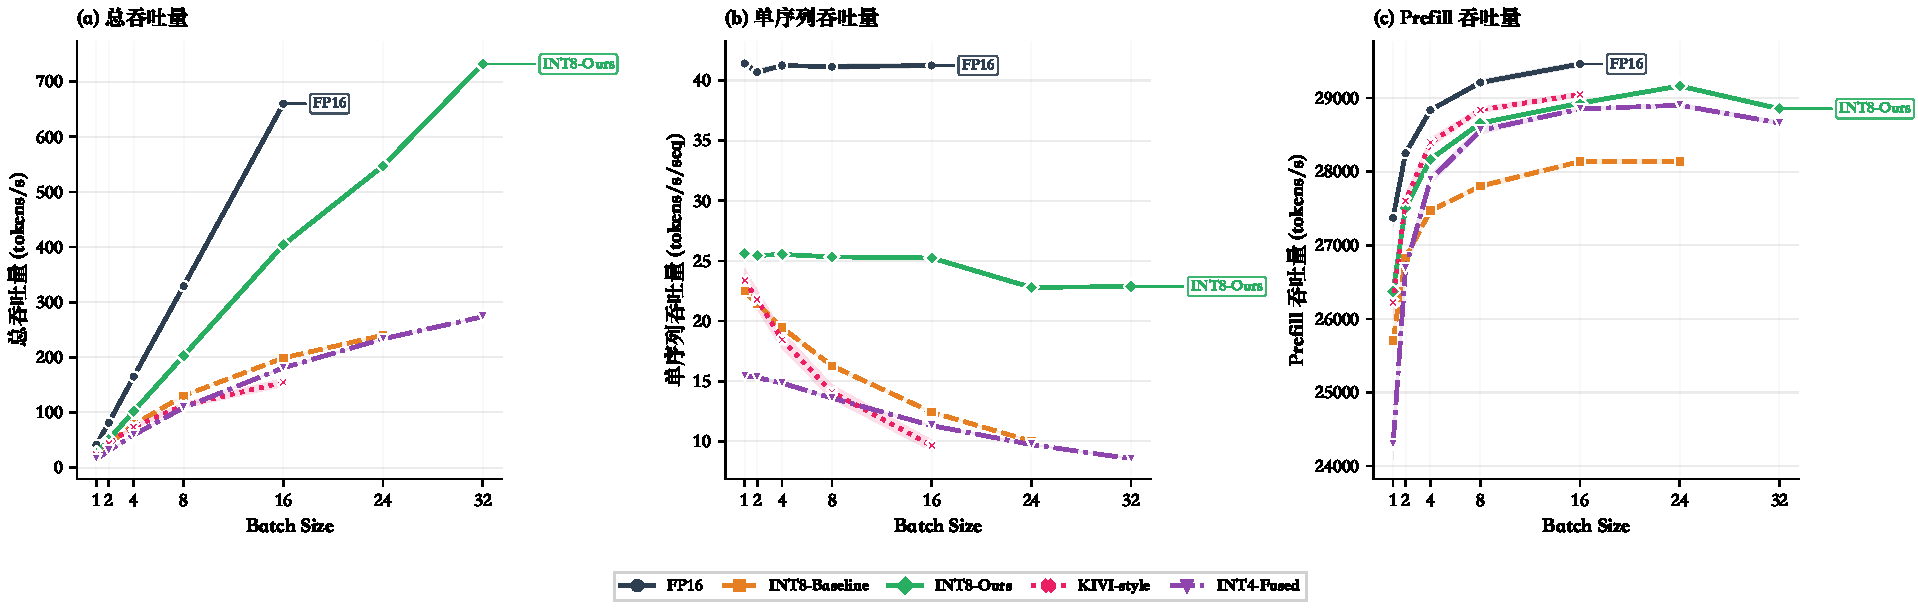
\includegraphics[width=0.9\textwidth]{figures/appendix_throughput_dashboard.pdf}
  \caption{吞吐扩展性三联图（Qwen2.5-1.5B-Instruct，NVIDIA H20，序列长度 8192，生成长度 128）。
  面板（a）展示总吞吐量，面板（b）展示单序列吞吐量，
  面板（c）展示 prefill 吞吐量。统一图例和坐标轴用于观察当前后端组合下 batch 扩展中的并发收益与单序列代价。}
  \label{fig:app-throughput-dashboard}
\end{figure}

\begin{figure}[!htbp]
  \centering
  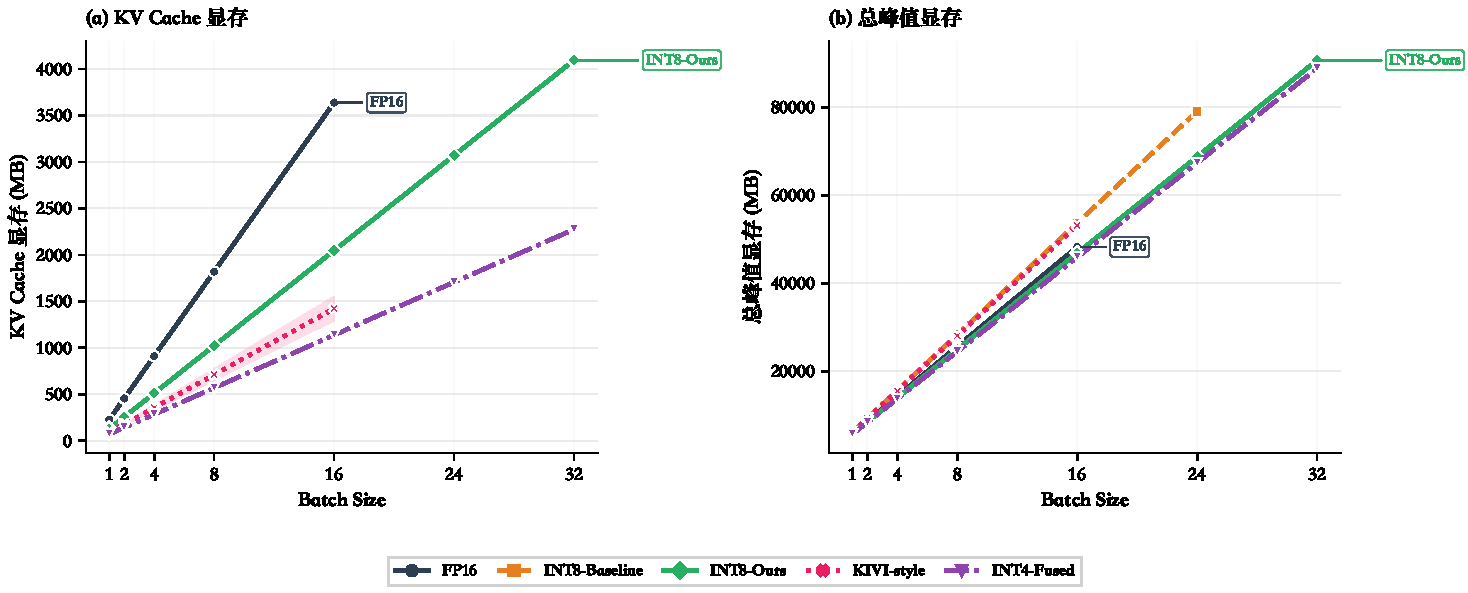
\includegraphics[width=0.9\textwidth]{figures/appendix_memory_dashboard.pdf}
  \caption{显存扩展性双联图（Qwen2.5-1.5B-Instruct，NVIDIA H20，序列长度 8192）。
  面板（a）展示 KV Cache 显存随 batch size 的线性增长，
  面板（b）展示总峰值显存；两者共同说明量化节省如何改变当前扫描范围内的可容纳 batch。}
  \label{fig:app-memory-dashboard}
\end{figure}

\phantomsection
\paragraph{批处理容量与 INT4-RoleAlign 扩展轨迹。}
\label{sec:app-batch-capacity}

表~\ref{tab:app-batch} 合并呈现 batch 维度的容量边界与扩展轨迹：
（a）各模式在序列长度 8192 条件下的已测最大可行 batch；
（b）INT4-RoleAlign 在不同 batch 下的 TPOT 与 KV Cache 显存。

\begin{table}[!htbp]
  \centering
  \caption{批处理扩展综合数据（Qwen2.5-1.5B-Instruct，NVIDIA H20，序列长度 8192，独占 GPU）}
  \label{tab:app-batch}
  \small
  \resizebox{\textwidth}{!}{%
  \begin{tabular}{lccc}
    \toprule
    \multicolumn{4}{l}{\textit{（a）各量化模式已测最大可行 batch（1--32 扫描）}} \\
    \midrule
    \textbf{量化模式} & \textbf{已测最大可行 batch} & \textbf{扫描范围} & \textbf{容量结论} \\
    \midrule
    FP16            & 16 & 1--16 & 范围内可行；未扩展至 32 \\
    INT8-Baseline   & 24 & 1--32 & batch=32 显存不足 \\
    INT8-Canonical  & 32 & 1--32 & 范围内可行 \\
    INT4-Baseline   & 16 & 1--16 & 范围内可行；未扩展至 32 \\
    INT4-Fused      & 32 & 1--32 & 范围内可行 \\
    INT4-RoleAlign  & 32 & 1--32 & 范围内可行 \\
    \midrule
    \multicolumn{4}{l}{\textit{（b）INT4-RoleAlign 批处理扩展轨迹（FP16 vs INT4-RA 对照）}} \\
    \midrule
    \textbf{Batch} & \textbf{TPOT FP16 / INT4-RA (ms)} & \textbf{KV FP16 / INT4-RA (MB)} & \textbf{KV 压缩比} \\
    \midrule
    1  & 24.78 / 60.18  & 227  / 60  & 3.78$\times$ \\
    4  & 24.65 / 73.17  & 910  / 242 & 3.76$\times$ \\
    8  & 24.21 / 93.07  & 1820 / 484 & 3.76$\times$ \\
    16 & 24.23 / 134.46 & 3640 / 968 & 3.76$\times$ \\
    \bottomrule
  \end{tabular}
  }

  \vspace{2pt}
  {\footnotesize 注：（a）在序列长度 8192、NVIDIA H20 与当前后端组合下，INT8-Canonical 与 INT4 融合模式均可支持已测 batch=32；INT8-Baseline 在 batch=32 时出现中间张量显存不足，因此容量边界从 24 移至 32 只相对于该 baseline 解释。（b）KV 压缩比约 3.76$\times$ 恒定；INT4-RoleAlign 的 TPOT 随 batch 增长，说明该实现仍有并发反量化摊销开销。batch=16 时其 KV Cache 为 968~MB（FP16 为 3640~MB），主要收益体现在容量边界而非速度主结论。}
\end{table}

% Supplementary deployment diagnostics.

% ============================================================
\section{INT4 失稳机制与评估粒度边界补充}
\label{sec:app-int4-mechanism-boundary}
% ============================================================

本节按四层组织 INT4 相关补充材料：首先用 Needle 深度--位置热力图给出
long-context cliff 的可视化背景；随后用 scale 精度敏感性读数排除
“scale dtype 单点失误”解释；第三部分保留噪声--长度交互的近似推导，给出
32K 场景下 INT4 阶跃退化的机制直觉；最后用 chunk size 消融界定评估粒度和
流式近似协议边界。最后一部分只限定协议适用范围，不引入新的主机制结论。

\phantomsection
\paragraph{Needle 深度--位置热力图补充。}
\label{sec:app-needle-heatmaps}
图~\ref{fig:app-needle-depth-grid} 补充展示 Needle 任务的深度位置热力图。
该图服务于正文第~\ref{subsec:ch4-int4-cliff}~节的阶跃崩塌模式：
它说明在当前热力图覆盖设置下，对称 INT4 的退化主要在长上下文与深层 needle 位置上被放大，
并为下文噪声--长度推导提供可视化背景。

\begin{figure}[!htbp]
  \centering
  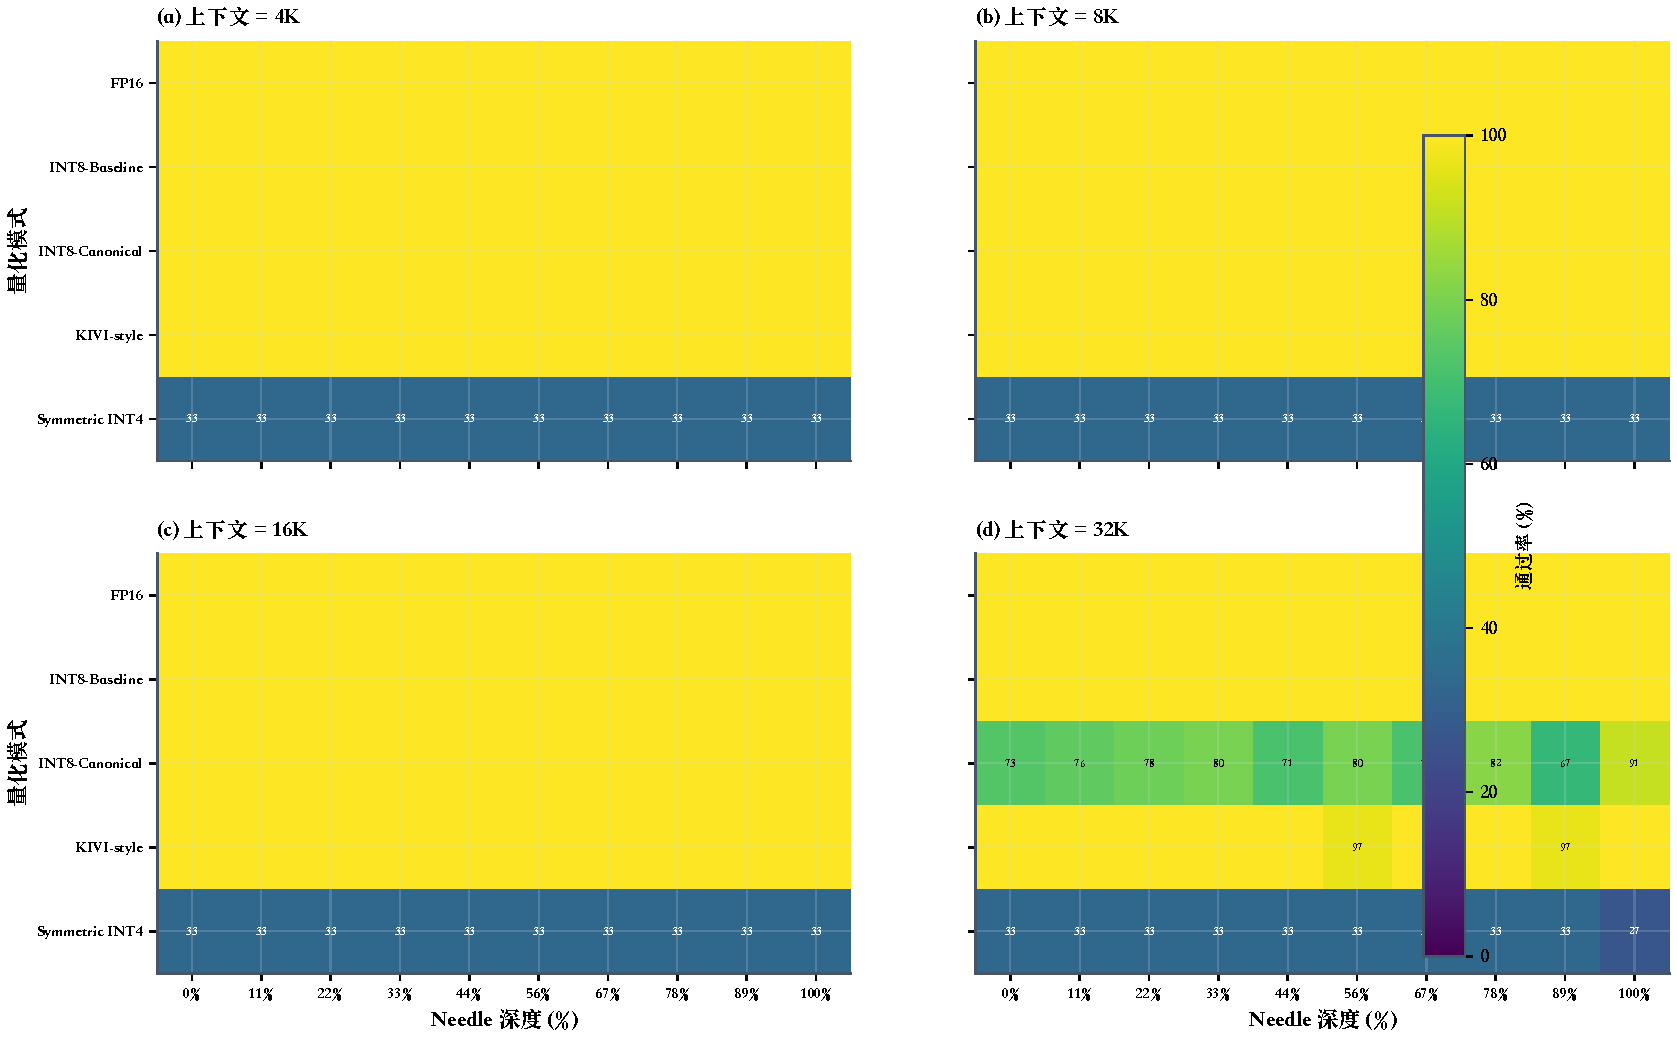
\includegraphics[width=\textwidth]{figures/needle_depth_grid.pdf}
  \caption{Needle-in-a-Haystack 深度-位置热力图总览。
  四个面板分别对应 4K、8K、16K 和 32K，并共享同一色标。
  该图用于定位 INT4 退化在上下文长度和 needle 深度上的放大位置，
  不替代正文的主表结论。}
  \label{fig:app-needle-depth-grid}
\end{figure}

精确匹配率（exact match）采用比通过率更严格的 Needle 判据，
其趋势与图~\ref{fig:app-needle-depth-grid} 一致：
FP16 在 4K--32K 均保持 100\%，INT8-Canonical 在 4K--16K 保持 100\%，
并在 32K 端点给出约 70.3\% 的长上下文边界读数；
对称 INT4 则在 4K 已显露边界，并在 8K 及以上区间构成长上下文边界对照。
这些 exact-match 读数作为严格判据补充图~\ref{fig:app-needle-depth-grid}，
不再作为独立视觉证据展开。

\paragraph{Scale 精度敏感性诊断。}
\label{sec:app-scale-precision}
表~\ref{tab:app-scale-precision} 是一组补充诊断读数，用于确认对称 INT4 失稳并非仅由
scale 存储精度不足造成。所有 scale 参数均以 float32 精度维护。
本节中的 behavior-guided 对称 INT4 不等同于正文主线的 INT4-RoleAlign 非对称路径。

\begin{table}[!htbp]
  \centering
  \caption{INT4 量化 scale 精度敏感性实验
    （32K 序列；PPL 为固定序列 likelihood，Needle 使用三个固定种子的贪婪生成）}
  \label{tab:app-scale-precision}
  \resizebox{\textwidth}{!}{%
  \begin{tabular}{llcccc}
    \toprule
    \textbf{模型} & \textbf{模式} & \textbf{PPL} & \textbf{Needle (\%)} & \textbf{校准} & \textbf{Scale dtype} \\
    \midrule
    \multirow{2}{*}{Qwen2.5-1.5B} & Symmetric INT4 baseline & 19.65 & 0 & percentile & float32 \\
                                    & Symmetric INT4 behavior-guided & 22.80 & 0 & KL proxy   & float32 \\
    \midrule
    \multirow{2}{*}{Qwen2.5-7B}   & Symmetric INT4 baseline & 86.56 & --- & percentile & float32 \\
                                    & Symmetric INT4 behavior-guided & 52.19 & --- & KL proxy   & float32 \\
    \midrule
    \multirow{2}{*}{LLaMA-3.1-8B} & Symmetric INT4 baseline & 6.97  & 100 & percentile & float32 \\
                                    & Symmetric INT4 behavior-guided & 7.64  & 100 & KL proxy   & float32 \\
    \bottomrule
  \end{tabular}
  }
  \begin{tablenotes}
    \footnotesize
    \item 注：7B Needle 未包含在该诊断消融中（标记 ---）。
    1.5B Needle 0\% 反映该模型在 32K 对称 INT4 下的边界；
    7B 基线 PPL=86.56 与正文同量级结果一致，说明该敏感性不是 scale dtype 单点造成。
  \end{tablenotes}
\end{table}

\textbf{补充读数。}
在同一 float32 scale 条件下，7B 的 behavior-guided 对称 INT4 PPL 低于 percentile baseline，
但 1.5B 的 Needle 仍为 0\%，LLaMA-3.1-8B 则在两种对称 INT4 配置下保持 100\%。
因此本节只支撑第~\ref{subsec:exp-int4-honest}~节的边界判断：
scale 精度是必要的数值卫生条件，但对称 INT4 cliff 还会受到模型结构与上下文长度调节。

\paragraph{量化噪声与序列长度交互效应。}
\phantomsection
\label{sec:app-sqnr-derivation}
本段提供正文第~\ref{subsec:exp-int4-honest}~节中量化步长与序列长度交互效应的近似分析。

Needle-in-a-Haystack 任务的检索成功条件可形式化为：
目标位置 $t$ 的 attention logit 与最强干扰位置的差值
$\delta = z_t - \max_{i \neq t} z_i$
（其中 $z_i = \bq^\top \bk_i / \sqrt{d_k}$）
需在量化后仍保持正值，使 softmax 将最大概率分配给目标位置。

当 Key 矩阵经 INT4 量化后，每个 logit $z_i$ 受到量化噪声扰动 $\epsilon_i$，
其方差约为：
\begin{equation}
  \text{Var}(\epsilon_i) \approx \|\bq\|^2 \cdot \sigma_{q,4}^2 / d_k
\end{equation}
其中 $\sigma_{q,4}^2 = \Delta_4^2 / 12$ 为 INT4 量化的逐元素噪声方差。

随序列长度 $n$ 增大，$\max_{i \neq t} (z_i + \epsilon_i)$ 的期望值
以 $O(\sqrt{2 \ln n} \cdot \sigma_\epsilon)$ 的速率增长（极值统计理论），
而目标信号 $\delta$ 不随 $n$ 增大。
在这一近似模型下，可以定义一个临界序列长度 $n^*$，满足：
\begin{equation}
  \delta \approx \sqrt{2 \ln n^*} \cdot \sigma_\epsilon
\end{equation}
当 $n > n^*$ 时，量化噪声超过目标 margin 的风险快速上升，检索失败概率随之增大。

在同一对称裁剪范围下，INT8 与 INT4 的 $q_{\max}$ 分别为 127 与 7，
因此 INT4 相对 INT8 的逐元素噪声方差比约为
$\sigma_{q,4}^2 / \sigma_{q,8}^2 = (127/7)^2 \approx 3.29\times 10^2$。
INT4 的 $n^*$ 远小于 INT8。该近似模型为 1.5B 模型上
从短上下文到 32K 的 Needle 通过率下降提供了理论直觉；
实际退化强度仍受模型结构、校准格式和注意力分布共同调节。


\paragraph{评估粒度鲁棒性。}
\phantomsection
\label{sec:app-chunksize}
本段验证量化粒度变化对低比特路径的影响。
前述各节采用 128-token chunk 协议；cs=1 则更接近每步都读写量化历史 KV 的 streaming decode。
表~\ref{tab:app-chunksize} 给出 Qwen2.5-1.5B-Instruct 上
三种粒度下 FP16、\mbox{INT4-RoleAlign} 和 KIVI-style INT4 的 PPL 对比。

\begin{table}[!htbp]
  \centering
  \caption{量化评估粒度敏感性（Qwen2.5-1.5B-Instruct，PPL，seed=1234）}
  \label{tab:app-chunksize}
  \resizebox{\textwidth}{!}{%
  \begin{tabular}{lccc}
    \toprule
    \textbf{配置} & \textbf{cs=128} & \textbf{cs=8} & \textbf{cs=1} \\
    \midrule
    FP16                     & 9.31 & 9.31 & 9.31 \\
    INT8-Canonical           & 8.95 & 9.34 (+0.3\%$^{\dagger}$) & 9.27 (-0.4\%$^{\dagger}$) \\
    \textbf{INT4-RoleAlign}  & \textbf{10.58} (+13.7\%) & \textbf{62.10} (+567\%) & $>$10{,}000$^{\star}$ \\
    KIVI-style INT4          & 10.43 (+12.0\%) & 60.54 (+550\%) & 10{,}332 (+110{,}900\%)$^{\star}$ \\
    \bottomrule
  \end{tabular}%
  }
\end{table}

\noindent\emph{表注与边界。}
括号内为相对 FP16 的 PPL 变化率，cs = chunk\_size。
$^{\dagger}$ INT8-Canonical 的 cs=128 PPL 低于 FP16，主要反映评测切分口径差异；
cs=1 相对 FP16 仍基本持平，说明更高量化级别提供了更大的 range 容错。
$^{\star}$ cs=1 下的极端 PPL 失效来自不含 FP16 Residual Buffer 的 per-channel K + per-token V 格式：
当每步都以单 token 建立 per-channel K scale 时，后续 token 极易超出 clamp 范围。
KIVI 原论文为 streaming decode 设计了 Residual Buffer（$R=128$）和 residual-group-scale 更新；
因此表中 KIVI-style 的 cs=1 数字只刻画本文简化基线与 INT4-RoleAlign 在无 residual buffer 条件下的共同边界，
不代表 KIVI 原论文方法在 streaming 设置下的性能上界。
该边界仅在 Qwen2.5-1.5B 单模型单种子条件下验证，并受上述实现范围限定。

% ============================================================
\section{K/V 精度消融与 MixedKV 跨模型补充数据}
\label{sec:app-kv-ablation-full}
% ============================================================

本节补充正文第~\ref{sec:exp-kv-sensitivity}~节中未展开的两类材料：
Mistral-7B 的 LongBench 数据源说明，以及 MixedKV 的逐模型边界读数。

\textbf{Mistral-7B LongBench 数据说明。}
Mistral-7B-Instruct-v0.3 在本组 K/V 消融与 MixedKV 补充评测中的 LongBench 结果均为 1.0，
包括 K/V 消融的三种配置（K-only, V-only, K4V8）
和 MixedKV 对比的三种方法（FP16, KIVI-style, MixedKV）。
该结果源于这组补充评测使用的 Mistral LongBench 合成数据源，
评分不反映模型的实际长文本理解能力，
因此在正文第~\ref{sec:exp-kv-sensitivity}~节的 K/V 跨模型 LongBench 对比中排除了 Mistral 的数据。
需强调的是，这一数据源异常影响的仅是 LongBench 评测本身，
而非量化方法。Mistral-7B 在 PPL、Needle 和 RULER 上的评测均正常有效。

\textbf{K/V 角色敏感性补充读数。}
在正文表~\ref{tab:ch4-kv-multitask} 的 LongBench 宏平均 F1（$\times$100）上，
K-only 与 V-only 两个诊断列分别为：
Qwen2.5-1.5B 的 $4.57 \pm 0.01$ 与 $4.54 \pm 0.04$，
Qwen2.5-7B 的 $4.10 \pm 0.11$ 与 $3.85 \pm 0.02$，
LLaMA-3.1-8B 的 $7.31 \pm 0.43$ 与 $6.21 \pm 0.66$。
Qwen 两个模型上的 K4V8 读数分别为 $2.58 \pm 0.08$ 与 $0.80 \pm 0.05$，
支持正文关于 Key 侧低精度更容易触发退化的判断；
LLaMA-3.1-8B 的 K4V8 LongBench 为 $8.92 \pm 0.79$，
说明任务级指标还会受到模型结构和数据协议共同调节。
因此本节只作为正文多指标诊断的补充，不把单一 LongBench 读数升级为独立结论。

\textbf{MixedKV 跨模型细节。}
\label{subsec:app-mixedkv-detail}
MixedKV 的逐模型表现进一步说明恢复强度具有架构依附性。
LLaMA-3.1-8B（$H_{kv}=8$）的 PPL 为 6.75（FP16 为 6.92），Needle 为 100\%，
RULER 为 33.28\%（FP16 为 31.48\%），LongBench 为 7.42\%（FP16 为 7.92\%）；
Qwen2.5-1.5B（$H_{kv}=2$）PPL 有轻度退化（9.37 vs 8.93），Needle 保持 100\%，
RULER 为 24.87\%（FP16 为 24.38\%）；
Qwen2.5-7B（$H_{kv}=4$）是当前 MixedKV 诊断中唯一出现 Needle 退化的模型（72.4\% vs FP16 100\%）。
Mistral-7B 的 PPL 5.20（FP16 为 5.19）和 RULER 53.67\%（FP16 为 53.98\%）均接近未量化基线，
但其 LongBench 读数因上述数据源问题不参与跨模型任务比较。

% ============================================================
\section{逐头温度校正诊断与 7B 校准目标溯源}
\label{sec:app-invtau-diagnostic}%
\label{sec:app-invtau-detail}

本节只承担两个附录功能：记录逐头温度校正 \(\tau^{-1}\) 的补充诊断动机，
并给出正文表~\ref{tab:ch4-kl-mse-convergence} 的 7B KL/MSE 数据溯源。
第三章与第四章的主线配置均不使用该组件，本节内容不构成默认组件。
\subsection{诊断性温度校正}
量化误差会扰动 logits $\bq\hat{\bK}^T / \sqrt{d_k}$ 并平坦化 softmax 分布；
逐头温度校正的诊断动机，是用层/头级缩放因子 \(\tau^{-1}_{l,h}\) 观察这种平坦化是否存在可补偿的架构依附性：
\begin{equation}
  \bm{p}_{\text{corrected}} = \softmax\!\left(\frac{\bq\hat{\bK}^T \cdot \tau^{-1}_{l,h}}{\sqrt{d_k}}\right)
  \label{eq:app-corrected-attn}
\end{equation}
其中 \(\tau^{-1}=1\) 退化为标准注意力。实现上，该缩放可等价写成 Query 预缩放：
\begin{equation}
  \text{Attn}(\bQ \cdot \tau^{-1},\; \hat{\bK},\; \hat{\bV})
  = \softmax\!\left(\frac{\bQ \hat{\bK}^T \cdot \tau^{-1}}{\sqrt{d_k}}\right) \hat{\bV}
  \label{eq:app-q-prescale}
\end{equation}
这一等价性说明 \(\tau^{-1}\) 可作为诊断开关接入现有 attention kernel。
但在非对称 RoleAlign 格式下，它没有形成稳定收益，因此只保留为补充诊断变体。

\subsection{7B KL vs MSE 校准目标趋同溯源}
\label{subsec:app-7b-kl-mse}
表~\ref{tab:app-7b-kl-mse} 是正文表~\ref{tab:ch4-kl-mse-convergence} 的溯源表。
它只说明 Qwen2.5-7B-Instruct 上 KL 与 MSE 目标已经趋同，不承担新的主结果宣称。
PPL 评测采用固定输入序列上的确定性 likelihood 累计，多 seed 只验证实现路径逐位一致性；规模依赖解释以正文讨论为准。

\begin{table}[!htbp]
  \centering
  \caption{7B KL vs MSE 校准对比数据溯源}
  \label{tab:app-7b-kl-mse}
  \small
  \begin{tabular}{lcccc}
    \toprule
    \textbf{校准目标} & $k\_\text{pct}$ & $v\_\text{pct}$ & \textbf{PPL} & \textbf{Seeds} \\
    \midrule
    KL-selected  & 100.0 & 99.9 & 7.1121 & 3 \\
    MSE-selected & 100.0 & 99.9 & 7.1121 & 3 \\
    FP16 (基线)   & ---   & ---  & 6.7097 & 1 \\
    \bottomrule
  \end{tabular}
\end{table}


% ============================================================
\section{Triton 融合核函数变体说明}
\label{sec:app-triton-variants}
% ============================================================

本节仅对正文第~\ref{sec:ch3-deployment}~节提及的 Triton 融合解码路径做实现变体说明，
其职责是给出不同变体的语义边界与复现角色，而不在附录中额外引入新的速度结论。
当前实现变体包括五类：INT8 融合解码主线实现、INT4 非对称融合核原型、
带自动调优的 INT4 迭代变体、显式兼容 GQA 头映射的 INT4 变体，
以及外部推理库适配层。这里按语义角色区分实现变体，不暴露具体文件名或实现代号。

这些变体在论文主线中的地位需要分层读取。
正文默认的系统落地主线是 INT8 融合核；
对 INT4-RoleAlign 而言，默认质量评测路径仍为参考解码实现，
非对称 Triton 变体仅承担实现可行性验证与后端扩展接口的角色。
因此，本附录补足“变体命名 / 实现角色 / 语义边界”的复核说明，
不把这些实现变体提升为正文主结果的直接来源。


% ============================================================
\section{Prompt-Adaptive Selector 探索性补充（future-work 起点）}
\label{sec:app-prompt-adaptive}
% ============================================================

本节汇总 prompt-adaptive selector 的探索性读数，
作为第~\ref{sec:conclusion-future}~节所列 per-prompt routing 方向的具体起点。
所有读数均使用同一 5-task 任务集，每个任务 50 个样本；
其中 8B 为正式探索矩阵，Qwen2.5-1.5B/7B 为同任务集下的补充读数。

\subsection{LLaMA-3.1-8B 五任务结果}
\label{sec:app-prompt-adaptive-8b}

8B 读数显示，prompt-adaptive selector 在 LCC 任务上取得局部正向信号：
其分数为 $11.36$，高于 auto-$k$ 的 $10.96$。
这一任务域信号提示，代码补全类输入可能为更细粒度的 prompt 级路由提供有价值的切入点。

\subsection{Qwen2.5-1.5B/7B 补充结果}
\label{sec:app-prompt-adaptive-offprotocol}

表~\ref{tab:app-prompt-adaptive-summary} 将三个模型上的 5-task mean 与局部信号并列展示。
该汇总不重新定义第四章主结果，只为 future work 中的 selector 设计空间提供模型规模与任务类型上的参照。

\begin{table}[!htbp]
  \centering
  \small
  \setlength{\tabcolsep}{5pt}
  \begin{tabularx}{\linewidth}{lcccX}
    \toprule
    \textbf{Model} & \textbf{fixed-$k$ mean} & \textbf{auto-$k$ mean} & \textbf{prompt-adaptive mean} & \textbf{局部读数} \\
    \midrule
    LLaMA-3.1-8B & \textbf{10.03} & 9.85 & 9.73 & LCC: prompt-adaptive $11.36$ vs auto-$k$ $10.96$ \\
    Qwen2.5-1.5B & 8.72 & \textbf{9.40} & 9.04 & auto-$k$ 与 prompt-adaptive 在 GovReport / DuReader 上读数一致 \\
    Qwen2.5-7B & 9.28 & \textbf{9.72} & 9.41 & auto-$k$ 与 prompt-adaptive 在 HotpotQA / GovReport / DuReader 上读数一致 \\
    \bottomrule
  \end{tabularx}
  \caption{Prompt-adaptive selector 的探索性 5-task 汇总。数值为各任务原生指标下的 mean；加粗表示该模型上的最高 mean。}
  \label{tab:app-prompt-adaptive-summary}
\end{table}

这些读数共同指向一个正向的后续设计问题：
prompt 级策略选择的收益可能集中在特定任务域与输入结构上，
而三组 5-task mean 的最高项仍分别落在 fixed-$k$ 或 auto-$k$ 上；
这说明当前 prompt-adaptive selector 更适合作为任务域线索的观察入口，
后续仍有空间进一步吸收任务类型、模型规模与 prompt 表征。
因此，本节将第~\ref{sec:conclusion-future}~节的 future-work 方向落到具体可检验现象上，不新增正文主结果。


% === 致谢 ===
% ============================================================
% acknowledgements.tex — 致谢
% ============================================================

\begin{acknowledgements}

本论文的完成离不开诸多师长、同学和亲友的关心与帮助，在此谨致以最诚挚的谢意。

首先，衷心感谢我的指导教师在本科毕业设计全过程中的悉心指导与严格要求。从选题确立、方案设计到论文撰写，老师始终给予了富有启发性的建议和耐心细致的修改意见，使我在科研方法与学术写作方面受益匪浅。

感谢实验室各位同学在日常学习与研究中的交流与协助。他们在实验方案讨论、代码调试和结果分析等方面提供的宝贵意见，对本文的完善起到了重要作用。

感谢华南理工大学提供的优良学术环境和计算资源支持，为本研究的顺利开展提供了坚实的基础保障。

最后，特别感谢我的家人多年来的无私支持与默默付出。他们的理解与鼓励是我坚持学业、完成论文的最大动力。

\end{acknowledgements}


\end{document}
